\documentclass[11pt,a4paper]{article}

\usepackage[margin=2.4cm]{geometry}
\usepackage{amsmath,amssymb}
\usepackage{graphicx}
\usepackage{booktabs}
\usepackage{siunitx}
\usepackage{float}
\usepackage{caption}
\usepackage{xcolor}
\usepackage[colorlinks=true,linkcolor=blue!60!black,urlcolor=blue!60!black,citecolor=blue!60!black]{hyperref}

\graphicspath{{figures/}}
\captionsetup{font=small,labelfont=bf,width=0.92\textwidth}
\sisetup{per-mode=symbol,range-phrase=--,range-units=single}

\newcommand{\vd}{v_{\mathrm{d}}}
\newcommand{\thref}{\theta_{\mathrm{ref}}}
\newcommand{\thdet}{\theta_{\mathrm{det}}}
\newcommand{\Tsat}{T_{\mathrm{sat}}}
\newcommand{\umns}{\micro\meter\per\nano\second}

\title{\textbf{MX17 Detector~3 --- June 2026 Cosmic-Bench Deep Dive:}\\[2mm]
       micro-TPC angle correlation, drift-velocity measurement,\\
       drift-gap determination, and gas diagnosis}
\author{Cosmic-bench analysis, Saclay\\[1mm]
        \small runs \texttt{mx17\_det3\_saturday\_scan\_6-27-26} and
        \texttt{mx17\_det3\_p2\_det1\_overnight\_6-27-26}}
\date{2 July 2026 --- rev.\ 4 July 2026 (drift velocity, waveforms, gap \&
gas: geometry estimator supersedes all time-based fits)}

\begin{document}
\maketitle

\begin{abstract}
\noindent
We analyse the final det3 weekend campaign: a \SI{2.4}{h} run at the
operating point (resist \SI{490}{V}, drift \SI{1000}{V}; configured for
\SI{12}{h} but stopped early for the overnight p2 run), a six-point drift-HV
scan (\SIrange{100}{1100}{V}), and two resist-HV scans.  Four results:
(i)~the universally observed \emph{off-diagonal} micro-TPC angle correlation is
quantitatively explained as an additive charge-spreading bias,
\(\tan\thdet \simeq \tan\thref \pm w/z_{\mathrm{rec}}\) with a spreading
width \(w \approx \SI{2}{mm}\) --- a detector constant, not a rotation and
not an analysis bug;
(ii)~\emph{every} time-based track fit --- the production fit and four
independent waveform-level estimators --- is biased low by
\SIrange{10}{20}{\percent} through prompt charge sharing between
neighbouring resistive strips; the mechanism is demonstrated strip-by-strip
in the raw waveforms and closed with a signal-formation simulation, which
validates a \emph{geometry} estimator (cluster-extent slope over time-span
plateau) as unbiased.  The result is
\(\vd(\SI{1000}{V}) = \SI{34 \pm 1.5}{\umns}\), with
\SIrange{1}{3}{\percent} statistical precision per 15-minute scan point.
Deconvolving the measured sharing from the waveforms (``unsharing'') makes
the time-based fits agree with geometry and, with one additive calibration
constant per plane, yields final micro-TPC angles with
\SI{0.19}{\degree} plateau bias and \SI{1.9}{\degree} resolution;
(iii)~the drift gap is mechanically \(\approx\SI{30}{mm}\), but only the
\(\approx\SI{23}{mm}\) of drift column closest to the mesh produces
recorded signal: the strip amplitude decays with drift \emph{depth}
(\(\lambda \approx \SIrange{16}{18}{mm}\), one universal curve across
drift fields) --- charge from the top of the gap is lost to
\textbf{attachment} plus threshold in the contaminated gas;
(iv)~the geometry-based \(\vd(E)\) at the \SI{30}{mm} field scale matches
Magboltz for Ar/iso 95/5 + \SIrange{1.0}{1.1}{\percent} H\(_2\)O
(+\,$\sim$\SI{1}{\percent} air) at RMS \SI{0.84}{\umns}, and the measured
attachment length matches the accompanying
\SIrange{0.15}{0.25}{\percent} O\(_2\) --- one air/moisture contamination
explains both anomalies.  Clean gas, mixing errors, and a wrong bottle of
Ar/CO\(_2\) 90/10 are all excluded (the last by \(+\SI{50}{V}\) at iso-gain
and zero attachment).
\end{abstract}

\tableofcontents

%=====================================================================
\section{Datasets, alignment and headline performance}
%=====================================================================

\subsection{Runs analysed}

All data were taken with det3 (\texttt{mx17\_3}, bulked June~15) in the
\emph{top} bench slot: FEU~7 = X strips, FEU~8 = Y strips, nominal
\(z=\SI{702}{mm}\), strip pitch \SI{0.78}{mm}, gas nominally
Ar/iC\(_4\)H\(_{10}\) 95/5 at atmospheric pressure
(Saclay, \(\approx\)\SI{745.8}{Torr}), non-zero-suppressed DREAM readout
(32~samples \(\times\) \SI{60}{ns} = \SI{1.92}{\micro s} window).

\begin{table}[H]
\centering\footnotesize
\setlength{\tabcolsep}{4pt}%
\begin{tabular}{llll}
\toprule
subrun & purpose & dur. & decoded statistics \\
\midrule
\texttt{long\_run\_resist\_490V\_drift\_1000V} & operating point & \SI{141}{min}
    & complete (4 files): 29k events, 47k M3 tracks \\
\texttt{drift\_scan\_...\_drift\_\{100..1100\}V} & drift scan, 6 pts & \SI{15}{min}
    & $\sim$5k M3 tracks / point \\
\texttt{hv\_scan\_resist\_\{425..525\}V} & resist scan 1, 11 pts & \SI{15}{min}
    & $\sim$2k clean rays / point \\
\texttt{hv\_scan2\_resist\_\{460..520\}V} & resist scan 2, 7 pts & \SI{15}{min}
    & $\sim$2k clean rays / point \\
\midrule
\texttt{long\_run\_p2\_det1\_sanity\_check} & overnight (p2 run) & ---
    & 53k rays; current headline det3 \\
\bottomrule
\end{tabular}
\caption{Weekend det3 datasets. The Saturday long run was configured for
\SI{720}{min} but was stopped after \SI{141}{min} (trigger-timestamp span;
the p2 overnight run started at 01:33 on the same bench) --- its 4 file pairs
are the complete dataset.}
\label{tab:datasets}
\end{table}

\subsection{Alignment}

The long run is aligned to the M3 reference tracker with the standard
iterative $z$/rotation/translation procedure (spark veto at 50 strips,
clean-cluster subset for the geometry fit).  Both weekend runs converge to the
\emph{same} geometry --- $z = \SI{714}{mm}$, $\theta = \SI{89.45}{\degree}$,
translation offsets agreeing to \SI{10}{\micro m} --- confirming the detector
did not move between runs.  The long-run alignment is therefore used as the
seed for every scan point, with only a translation refit per point (observed
shifts $<\SI{0.1}{mm}$).

\subsection{Headline performance}

\begin{figure}[H]
\centering
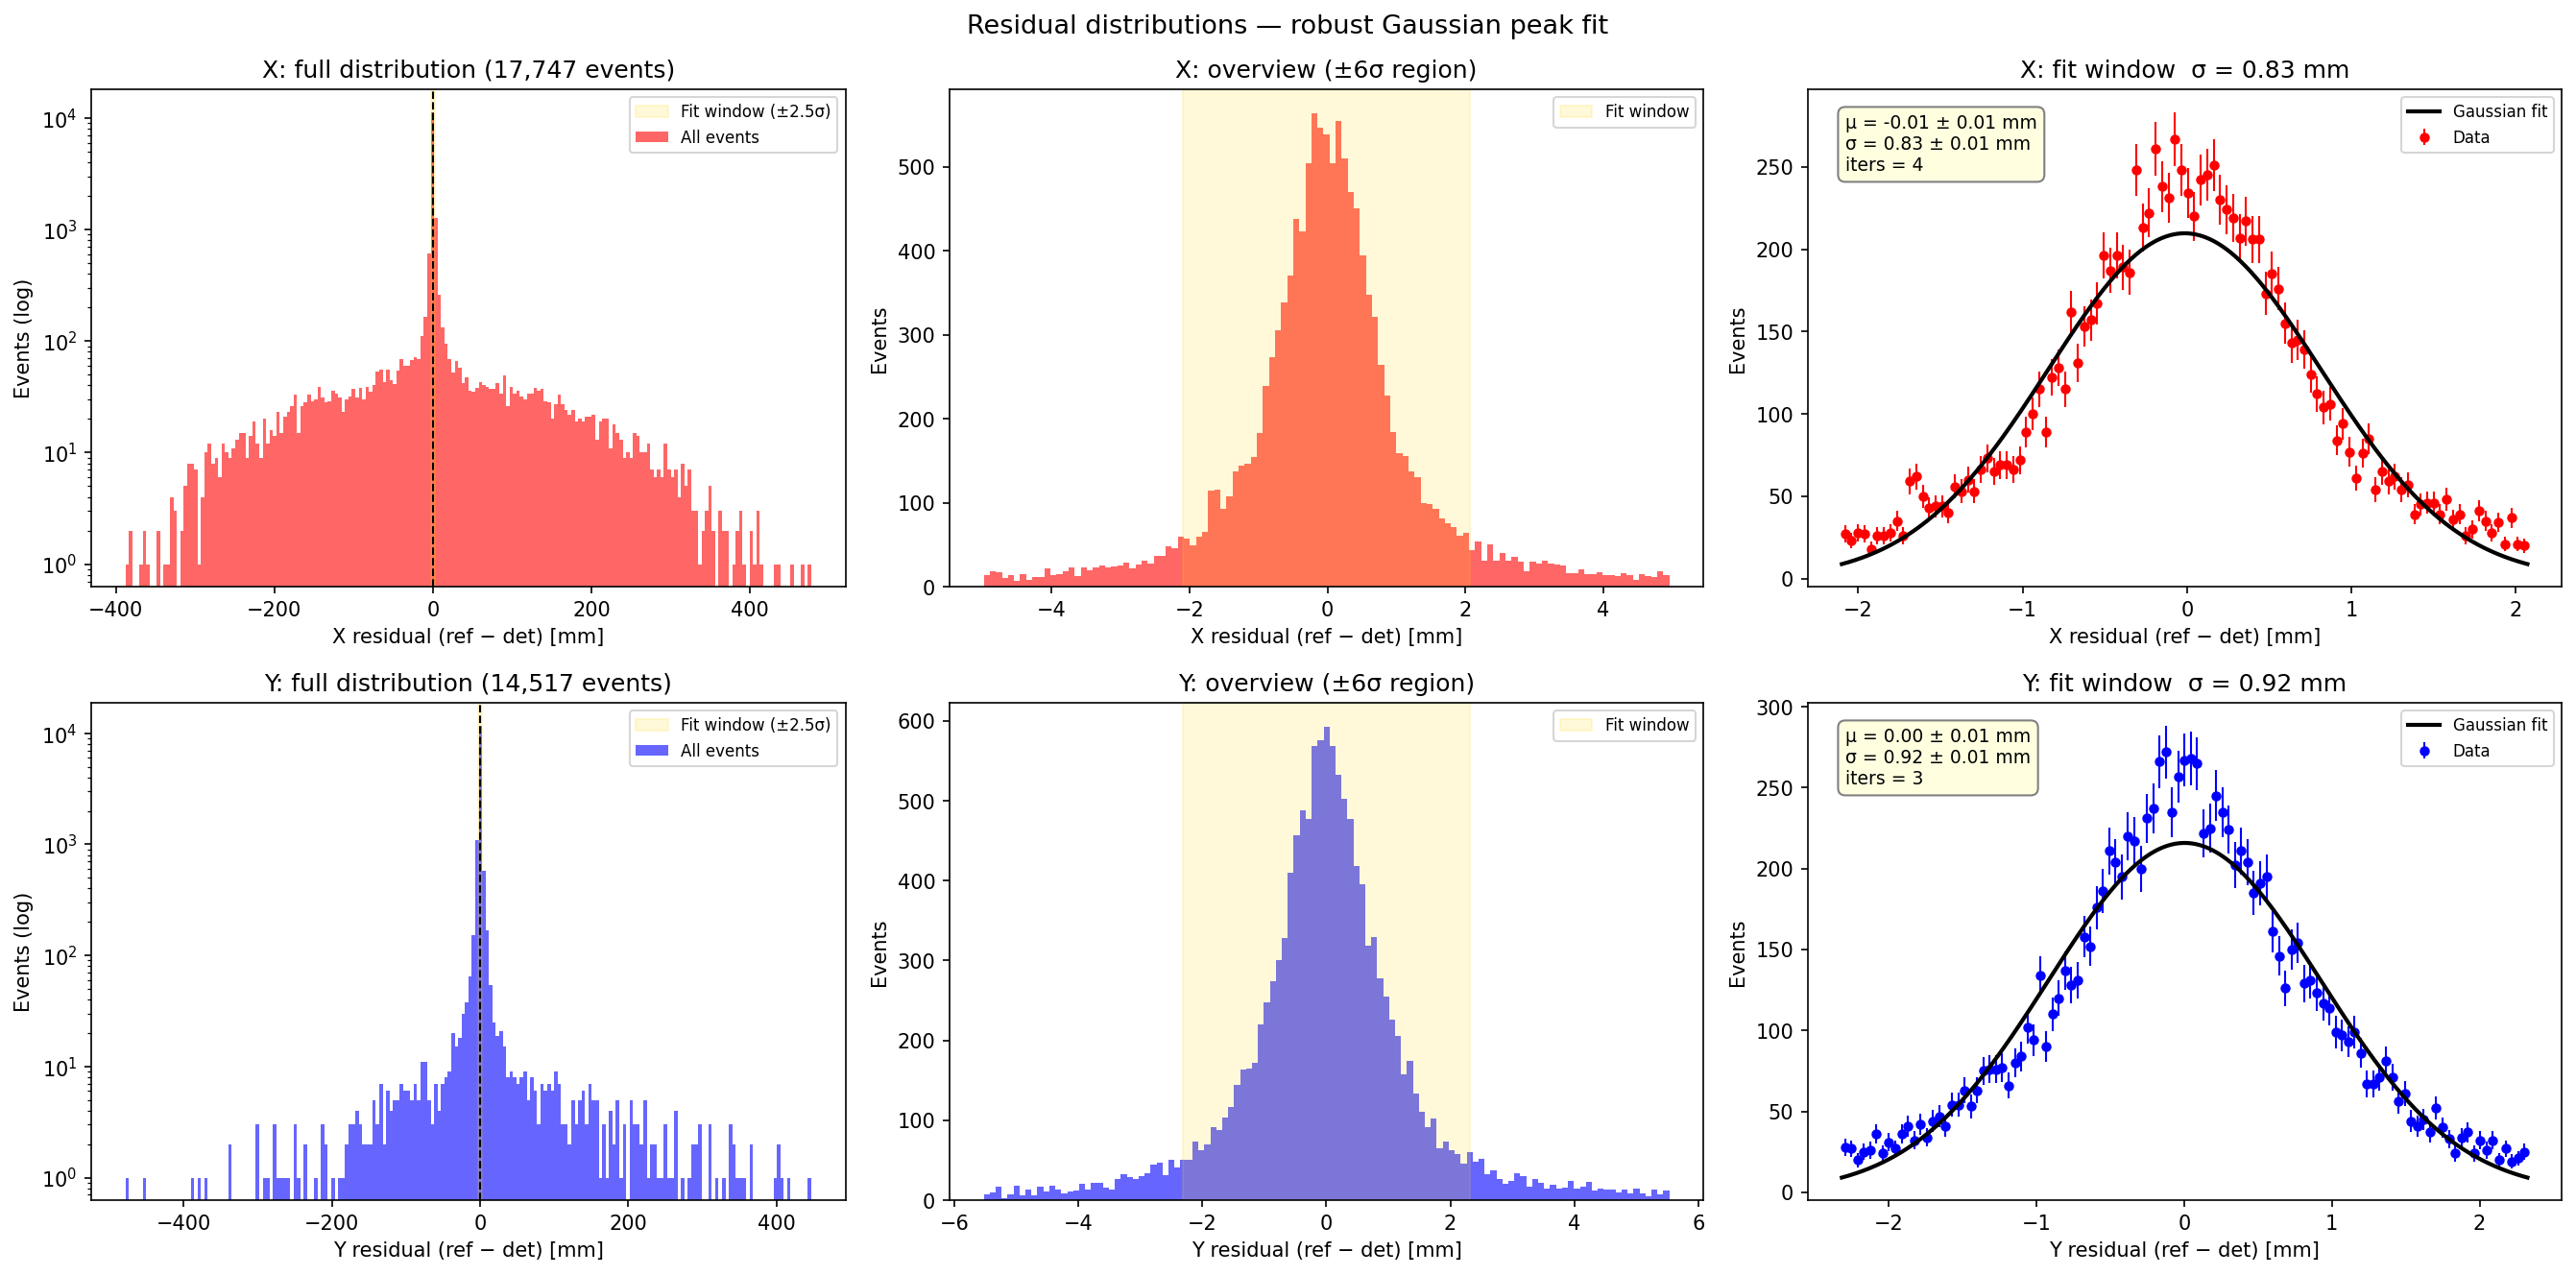
\includegraphics[width=\textwidth]{residuals.png}
\caption{Saturday long run: residuals between the aligned detector hit and
the projected M3 track.  The Gaussian core gives
$\sigma_x = \SI{0.83}{mm}$, $\sigma_y = \SI{0.92}{mm}$.}
\label{fig:residuals}
\end{figure}

From the efficiency breakdown of the Saturday long run (fixed active box,
clean M3 single tracks, $R=\SI{5}{mm}$ matching): the detector fires on
\SI{97.6}{\percent} of through-going muons, reconstructs an X+Y point for
\SI{80.2}{\percent}, and \SI{65.8}{\percent} land within \SI{5}{mm} of the
track (a \SI{14.4}{\percent} \emph{reco-far} tail).  The higher-statistics p2
overnight run gives the June-headline \SI{79.7}{\percent} within \SI{5}{mm}
with a much smaller tail; the difference (larger far tail in the Saturday
run) correlates with the higher spark fraction at resist \SI{490}{V}
(Sec.~\ref{sec:hvscans}) and can be probed further with the p2 dataset.
Either way det3 remains the best detector of the June batch, at
sub-mm core resolution in both slots and both weekends.

%=====================================================================
\section{The micro-TPC measurement}
%=====================================================================
\label{sec:utpc}

\subsection{Principle}

A single conversion/drift gap of depth $g$ sits above the micromesh; the
avalanche charge is read out on strips of pitch $p=\SI{0.78}{mm}$
(Fig.~\ref{fig:principle}).  A muon crossing at angle $\theta$ (measured from
the detector normal, i.e.\ from the drift direction) leaves an ionisation
trail spanning the \emph{full} gap in $z$ and $g\tan\theta$ in $x$.  (In this
detector, as Sec.~\ref{sec:gap} shows, only the fraction of the column within
$z_{\mathrm{rec}}\approx\SI{23}{mm}$ of the mesh survives the drift with
enough charge to be recorded --- everywhere below, ``the gap'' as seen by the
strips means this \emph{visible column} $z_{\mathrm{rec}}$, not the
\SI{30}{mm} electrode spacing.)  Electrons
drift to the mesh at velocity $\vd$, so the strip at horizontal distance
$\Delta x$ from the track's mesh-crossing point receives its charge later by
\begin{equation}
  \Delta t \;=\; \frac{\Delta z}{\vd} \;=\; \frac{\Delta x}{\vd\tan\theta}.
  \label{eq:utpc}
\end{equation}
Fitting strip signal time versus strip position (amplitude-weighted straight
line, anchored at the earliest hit) yields a slope whose inverse is
\begin{equation}
  \frac{\mathrm{d}x}{\mathrm{d}t} \;=\; \vd\tan\theta
  \qquad\Longrightarrow\qquad
  \tan\thdet \;=\; \frac{1}{\vd}\,\frac{\mathrm{d}x}{\mathrm{d}t}.
  \label{eq:angle}
\end{equation}
Equation~\eqref{eq:angle} is the micro-TPC angle estimator: it needs the
drift velocity $\vd$ as an external input, and conversely, once an external
reference ($\thref$ from M3) is available, the \emph{correlation between
$\thdet$ and $\thref$ measures $\vd$}.  That is the core idea exploited
throughout this note.  In the analysis code the raw fit slope is
$s \equiv \mathrm{d}x/\mathrm{d}t$ in \si{\umns}; the detector-frame slope
vector $(s_x, s_y)$ is rotated by the alignment angle
($\theta_{\mathrm{align}} \approx \SI{90}{\degree}$) into the M3 frame before
any comparison, so det-X pairs with ref-Y and vice versa.

\begin{figure}[H]
\centering
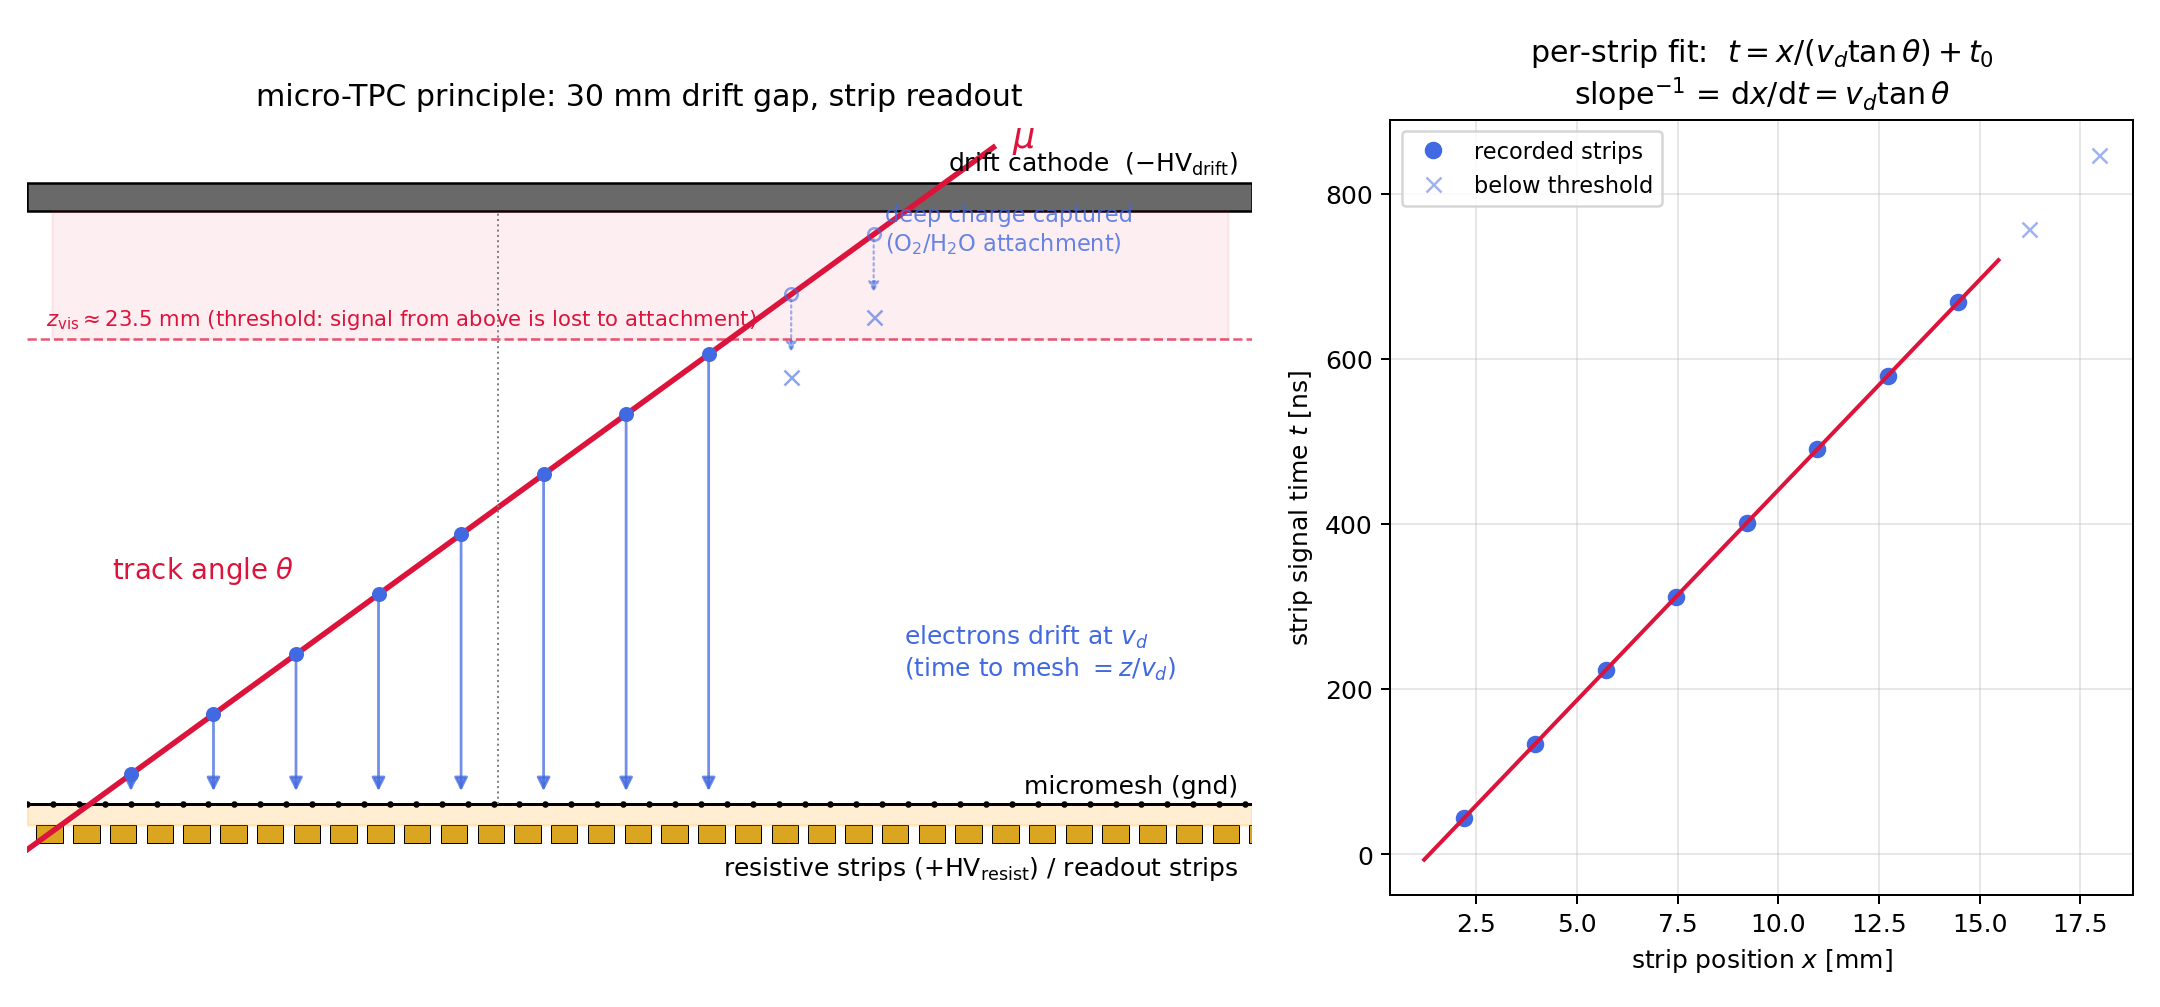
\includegraphics[width=\textwidth]{diagram_principle.png}
\caption{Micro-TPC principle. Left: an inclined muon (red) ionises the gas
along the full \SI{30}{mm} drift gap; electrons (blue) drift down at $\vd$
and arrive at the mesh with delays proportional to their production height.
Charge from above $z_{\mathrm{rec}}\approx\SI{23}{mm}$ (pink band) is lost
to attachment during the drift (Sec.~\ref{sec:gap}). Right: the per-event fit
of strip time vs.\ strip position over the recorded strips; the inverse slope
is $\vd\tan\theta$.}
\label{fig:principle}
\end{figure}

\subsection{Why the micro-TPC mode matters here}

Position resolution (Fig.~\ref{fig:residuals}) uses only the charge centroid
and is insensitive to everything discussed below.  The micro-TPC \emph{slope},
however, is the detector's unique selling point --- per-plane track angles
from a single thin detector --- and it is exactly this quantity that shows the
systematic effects analysed next.

%=====================================================================
\section{Why the angle correlation is always off-diagonal}
%=====================================================================
\label{sec:offdiag}

\subsection{The observation}

Figure~\ref{fig:anglecorr} shows the production angle-correlation plot for the
Saturday long run: reference angle $\thref$ (M3) versus detector angle
$\thdet$ (Eq.~\ref{eq:angle}, with $\vd$ set by the production
diagonal-projection scan).  The correlation is strong --- the micro-TPC works
--- but three features stand out, and they appear \emph{identically in every
detector of the June campaign} (det2 shown for comparison in
Fig.~\ref{fig:det2corr}):

\begin{enumerate}
  \item the dense ridge runs \emph{parallel} to the $y=x$ diagonal but is
        displaced \emph{outward}: $|\thdet| > |\thref|$ by
        $\sim$\SIrange{5}{6}{\degree};
  \item there are essentially \emph{no} events with
        $|\thdet| \lesssim \SI{5}{\degree}$ --- an exclusion gap around the
        vertical;
  \item events with $\thref \approx 0$ form \emph{horizontal arms} extending
        to large $|\thdet|$ of either sign.
\end{enumerate}

\begin{figure}[H]
\centering
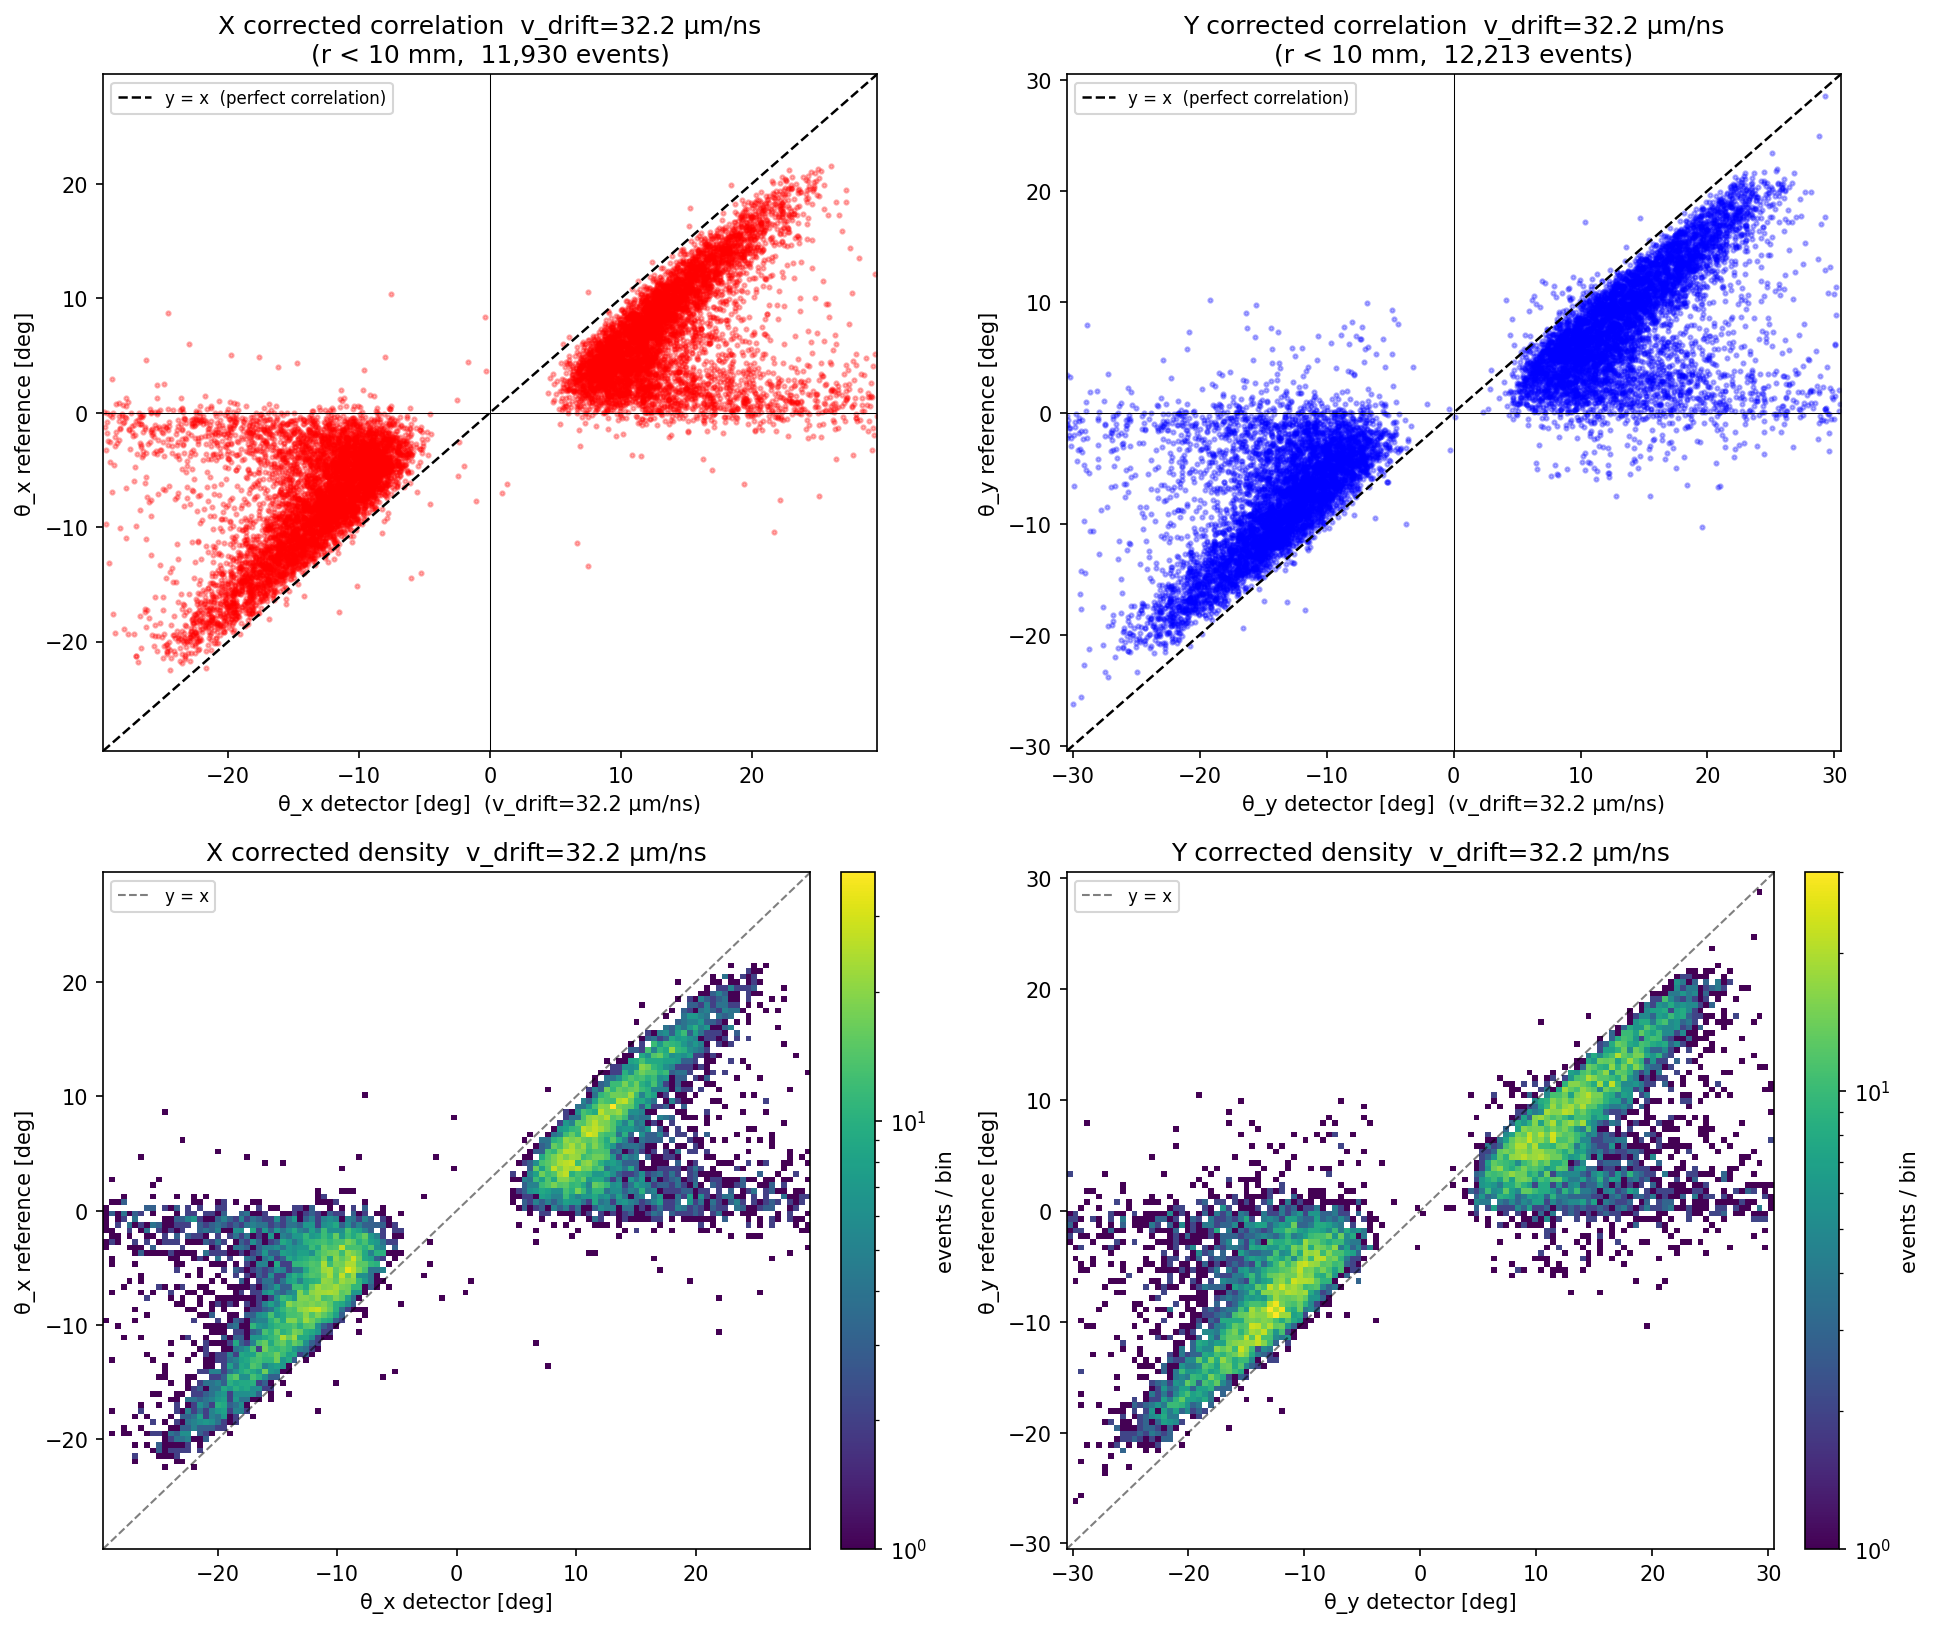
\includegraphics[width=0.94\textwidth]{angle_correlation_corrected.png}
\caption{Saturday long run, production angle correlation (top: scatter;
bottom: log-density) for the X (left) and Y (right) projections, using the
$\vd$ from the production $\sigma$-scan. The ridge is parallel to, but
displaced outward from, the dashed $y=x$ diagonal; note the empty band
$|\thdet|\lesssim\SI{5}{\degree}$ and the horizontal arms at
$\thref\approx 0$.}
\label{fig:anglecorr}
\end{figure}

\begin{figure}[H]
\centering
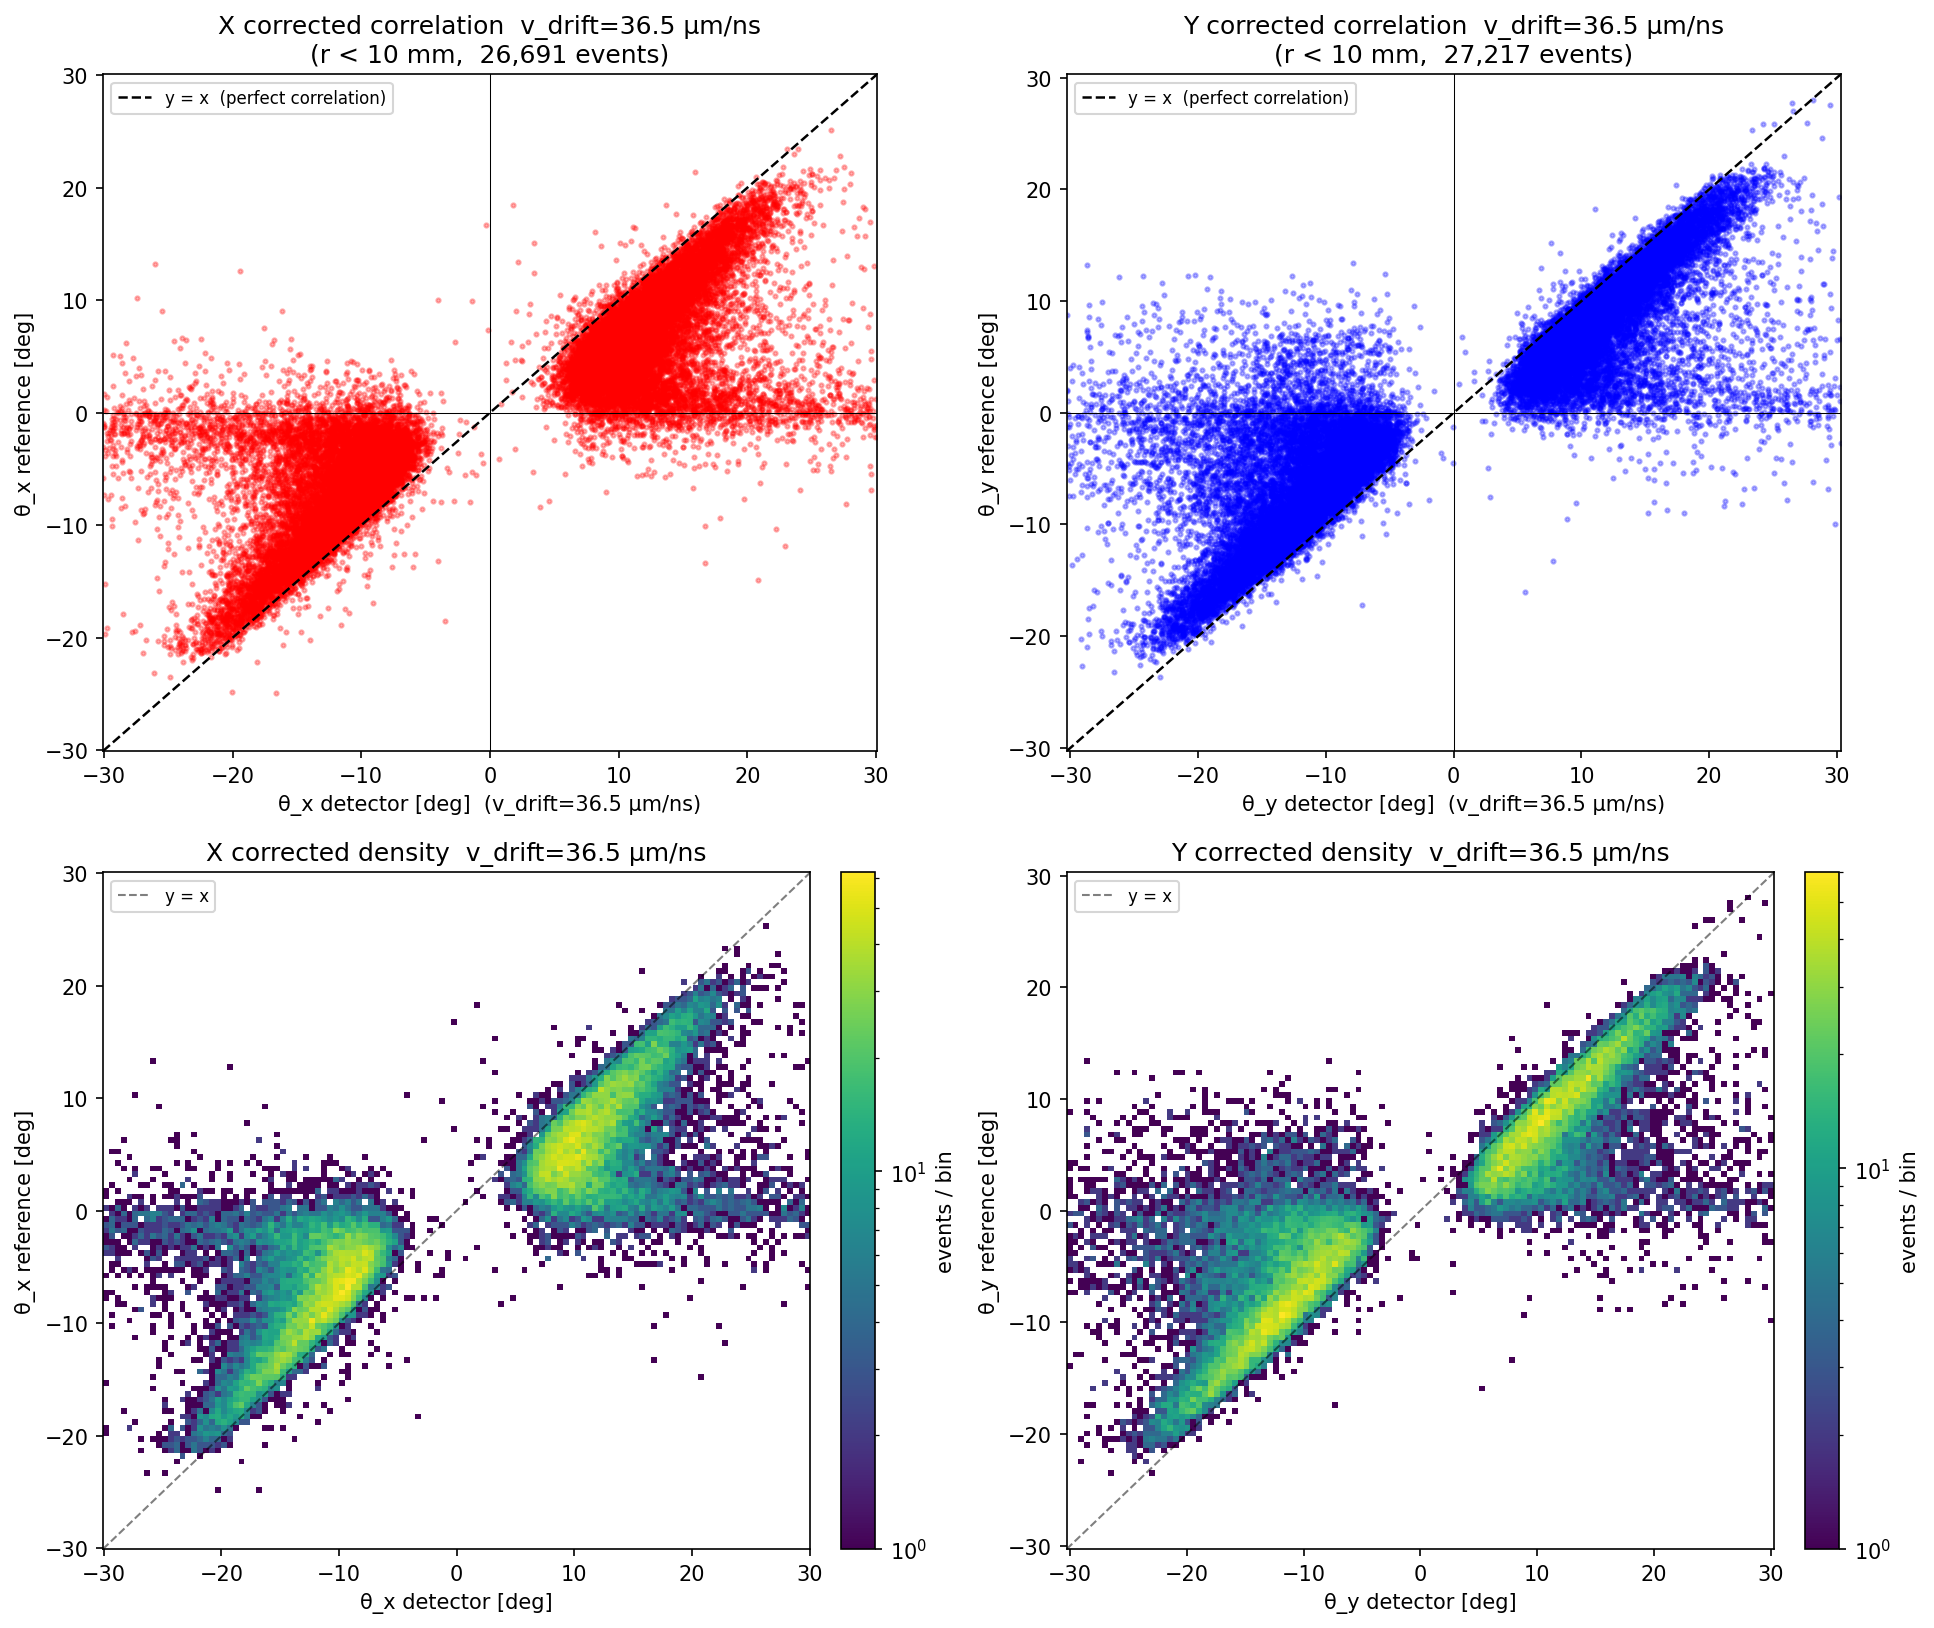
\includegraphics[width=0.94\textwidth]{det2_angle_correlation_corrected.png}
\caption{Same plot for \emph{det2} (6-22 overnight run). The off-diagonal
structure is identical --- this is a property of the detector family, not of
one chamber.}
\label{fig:det2corr}
\end{figure}

\subsection{Why it is \emph{not} a rotation or misalignment}

A residual in-plane rotation is absorbed by the alignment (the rotation scan
converges to \SI{0.05}{\degree} steps and the slope vector is rotated
accordingly).  More fundamentally, \emph{any} rotation or constant angular
offset would shift the correlation in \emph{one} direction --- up or down ---
whereas the observed displacement \textbf{flips sign with the track
direction}: tracks leaning one way reconstruct too steep in that direction,
tracks leaning the other way too steep in the other.  The offset is odd in
$\theta$, i.e.\ it behaves like $\;\mathrm{sign}(\theta)\cdot\mathrm{const}$,
which no rigid-body transformation produces.  An out-of-plane tilt of the
detector would also be a one-directional shift, and is excluded for the same
reason.

\subsection{The mechanism: fixed time span, inflated cluster width}
\label{sec:mechanism}

The key geometric fact (Fig.~\ref{fig:offsetdiagram}): \textbf{every cosmic
crosses the full drift gap}, so the recorded cluster always spans the entire
\emph{visible} column depth $z_{\mathrm{rec}}$ in $z$ (the fixed depth at
which drifting charge drops below threshold; Sec.~\ref{sec:gap}).
Consequently the \emph{time} extent of every cluster is the same,
\begin{equation}
  \Delta t_{\mathrm{cluster}} \;\approx\; \Tsat = z_{\mathrm{rec}}/\vd,
  \qquad \text{independent of } \theta,
\end{equation}
while the \emph{spatial} extent is
\begin{equation}
  \Delta x_{\mathrm{cluster}} \;\approx\;
  \underbrace{z_{\mathrm{rec}}\tan\theta}_{\text{geometric}}
  \;+\; \underbrace{w}_{\text{non-geometric}},
\end{equation}
where $w$ collects everything that widens the charge footprint on the strips
without carrying drift-time information: charge spreading across the
resistive layer, transverse diffusion, capacitive coupling to neighbours, and
$\delta$-electrons.  The fitted slope is then, schematically (writing
$z_{\mathrm{r}} \equiv z_{\mathrm{rec}}$),
\begin{equation}
  \frac{\mathrm{d}x}{\mathrm{d}t}
    \;\approx\; \frac{z_{\mathrm{r}}\tan\theta + w\,\mathrm{sign}(\theta)}{z_{\mathrm{r}}/\vd}
    \;=\; \vd\left(\tan\theta \pm \frac{w}{z_{\mathrm{r}}}\right)
  \qquad\Longrightarrow\qquad
  \boxed{\;\tan\thdet \;\approx\; \tan\thref \pm \frac{w}{z_{\mathrm{rec}}}\;}
  \label{eq:offset}
\end{equation}
an \textbf{additive, angle-independent excess in tan-space} whose sign
follows the track sign.  (The sign attaches to $w$ because the fit interprets
the extra width as extra track length in the direction the track already
leans; for a perfectly vertical track the sign is random --- hence the
horizontal arms.)

\begin{figure}[H]
\centering
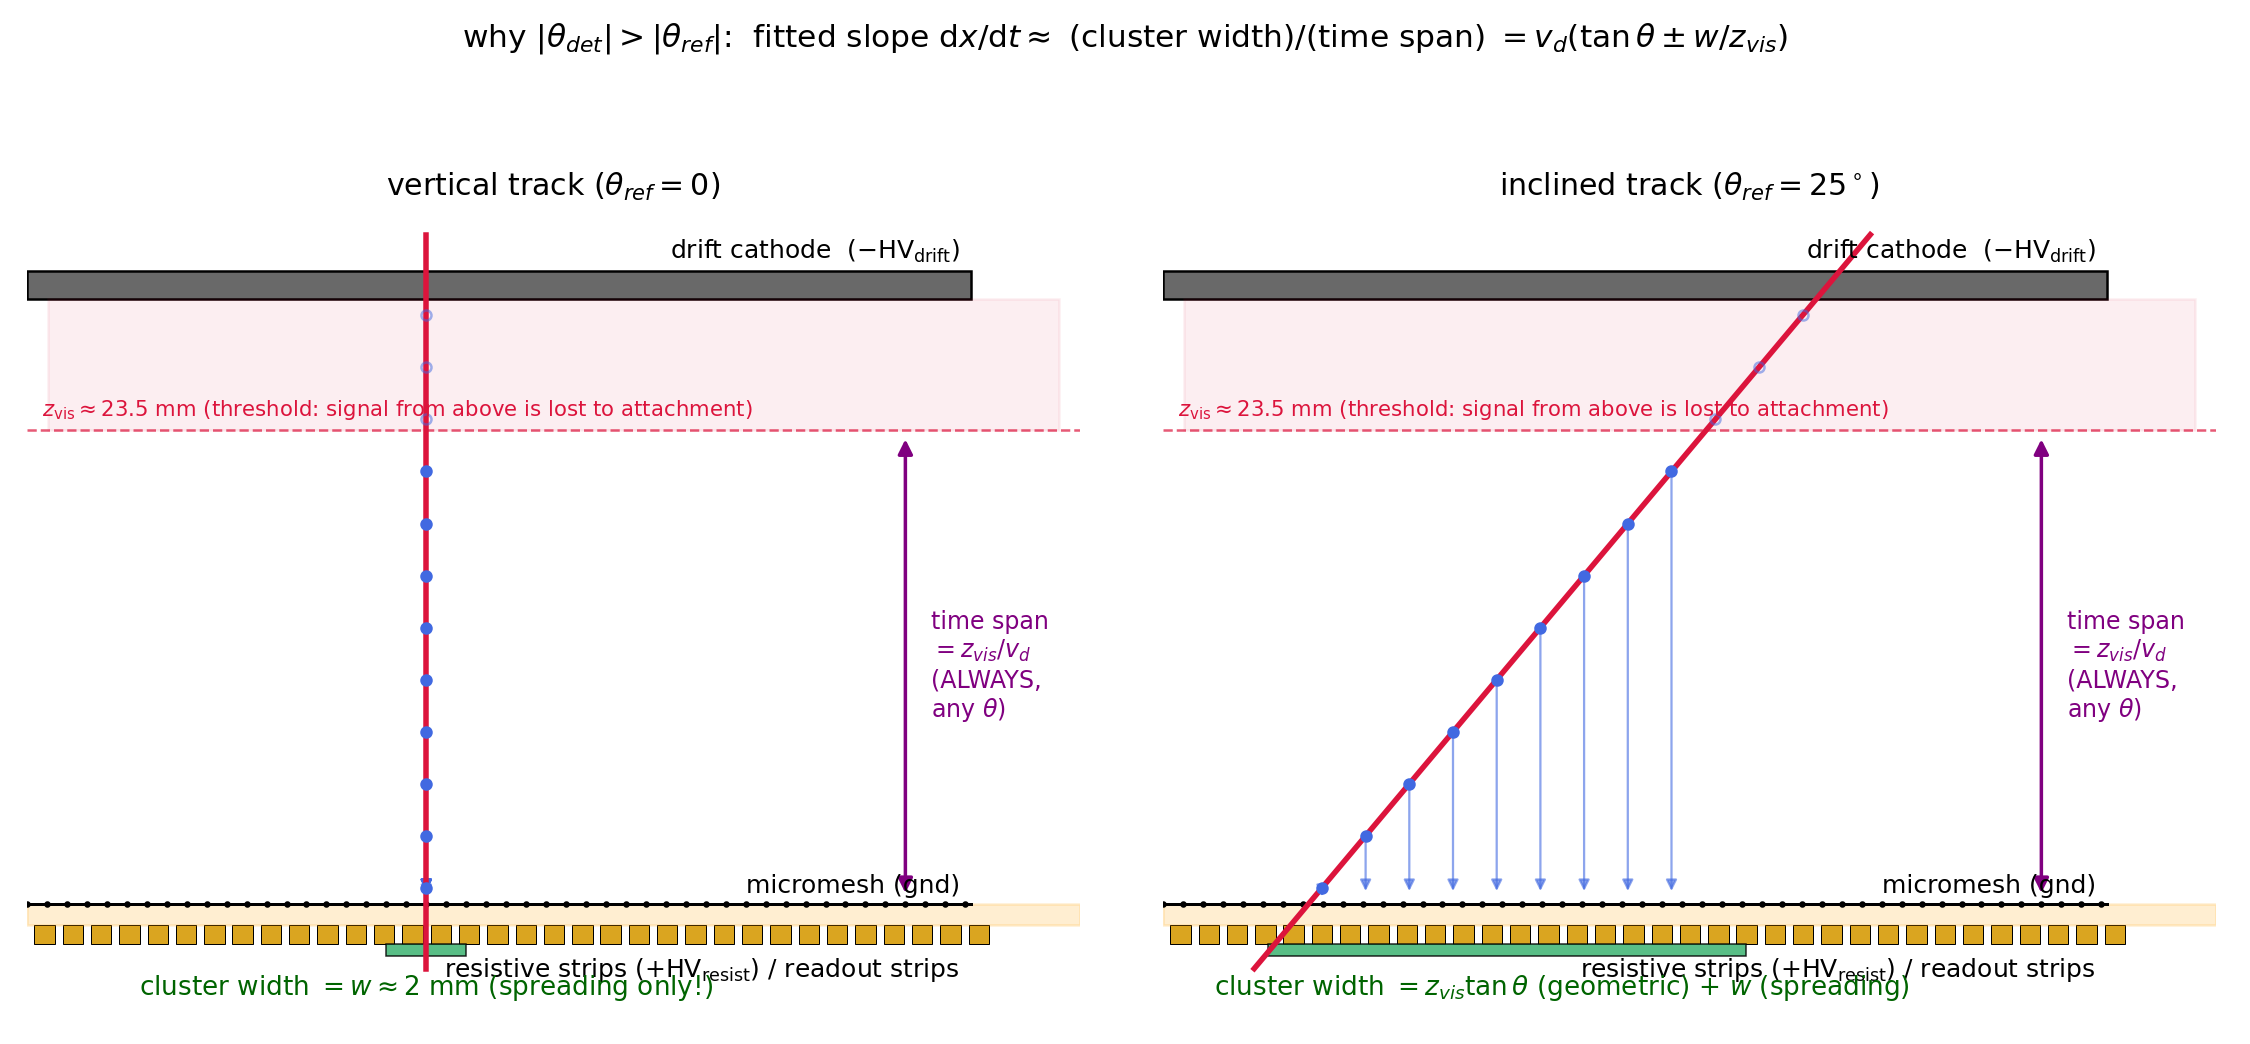
\includegraphics[width=\textwidth]{diagram_offset.png}
\caption{The off-diagonal mechanism. Left: a vertical track --- the time span
still covers the full visible column ($z_{\mathrm{rec}}/\vd$), but the
cluster width is pure spreading, $w\approx\SI{2}{mm}$; the fit converts $w$
into a fake angle $\arctan(w/z_{\mathrm{rec}})\approx\SI{6.5}{\degree}$ of
random sign. Right: an inclined track --- the width gains the geometric part
$z_{\mathrm{rec}}\tan\theta$, but $w$ still adds on top, always
\emph{increasing} $|\thdet|$.}
\label{fig:offsetdiagram}
\end{figure}

This single mechanism explains all three observations at once:
\begin{itemize}
  \item \textbf{parallel outward ridge}: Eq.~\eqref{eq:offset} is a constant
        displacement $w/z_{\mathrm{rec}}$ in tan-space; converted to degrees
        it is a nearly constant $\sim\arctan(w/z_{\mathrm{rec}})$ shift over
        the populated range;
  \item \textbf{exclusion gap}: no cluster can fit a slope smaller than
        $\sim w/z_{\mathrm{rec}}$, because even a vertical track's cluster is
        $w$ wide over a full-column time span ---
        $|\thdet| \gtrsim \arctan(w/z_{\mathrm{rec}})$ always;
  \item \textbf{horizontal arms}: for $\thref\approx 0$ the geometric width
        vanishes, the sign of the fitted slope is set by noise, and the
        magnitude is again $\sim w/z_{\mathrm{rec}}$ or larger (the events
        that pass the $\geq 4$-strip cut at small angle are precisely those
        with the largest spreading).
\end{itemize}
And because $w$ (a resistive-layer/diffusion property) and $z_{\mathrm{rec}}$
(set by the shared gas supply and thresholds, Sec.~\ref{sec:gap}) are common
to the whole detector family, \textbf{every chamber shows the same
off-diagonal pattern} --- exactly what is observed.

\subsection{Quantitative verification}

All of this is testable in the data of the 2.4\,h run
(\texttt{13\_tpc\_angle\_bias.py}); Figs.~\ref{fig:biasprofiles} and
\ref{fig:clustergeom}.  The ratios in this subsection are quoted in the
production time-fit frame ($\vd = \SI{28.1}{\umns}$, used to make these
plots); the $\sim$20\,\% velocity-scale correction of
Secs.~\ref{sec:vdrift}--\ref{sec:timing} rescales $\tan\thdet$ and
$w/z_{\mathrm{rec}}$ coherently and changes neither the mechanism nor the
spreading width $w$:

\begin{itemize}
  \item \textbf{the excess is flat in tan-space}: the median of
        $|\tan\thdet| - |\tan\thref|$ is constant at $w/z_{\mathrm{rec}} = 0.115$ for
        $|\thref| \gtrsim \SI{6}{\degree}$, in both planes
        (Fig.~\ref{fig:biasprofiles}, bottom row).
        $\arctan(0.115) = \SI{6.6}{\degree}$ --- the observed ridge
        displacement;
  \item \textbf{wider clusters carry more bias}: splitting by cluster size
        (\numrange{4}{6} / \numrange{7}{9} / $\geq$10 strips) orders the
        excess exactly as the spreading picture predicts;
  \item \textbf{the time span saturates}: the median cluster time span rises
        to a plateau $\Tsat \approx \SI{690}{ns}$ for
        $|\thref| > \SI{10}{\degree}$ --- the full-gap drift time
        (Fig.~\ref{fig:clustergeom}, top row).  (Its decrease towards
        $\theta=0$ is a per-strip integration effect: a vertical track's
        charge lands on few strips whose fitted times average over the
        column, shrinking the strip-to-strip span.);
  \item \textbf{the spatial width has a floor}: the median cluster extent at
        $\thref\approx 0$ is \SIrange{3}{5}{mm} where geometry predicts
        $\approx 0$; at larger angles it grows parallel to the geometric
        expectation $z_{\mathrm{rec}}\tan\theta$, offset by the same floor
        (Fig.~\ref{fig:clustergeom}, bottom row).
\end{itemize}

The ridge-fit intercepts (Sec.~\ref{sec:vdrift}) give the same number from a
completely different projection of the data:
$|b|/v = w/z_{\mathrm{rec}} = 0.115$, i.e.\
a spreading width $w = |b|\cdot\Tsat = \SI{2.2}{mm}$ ($\approx$3 strips),
a velocity-independent number.  Finally,
overlaying the parameter-free prediction of Eq.~\eqref{eq:offset} on the
measured density (Fig.~\ref{fig:withprediction}) tracks the ridge in both
planes.

\begin{figure}[H]
\centering
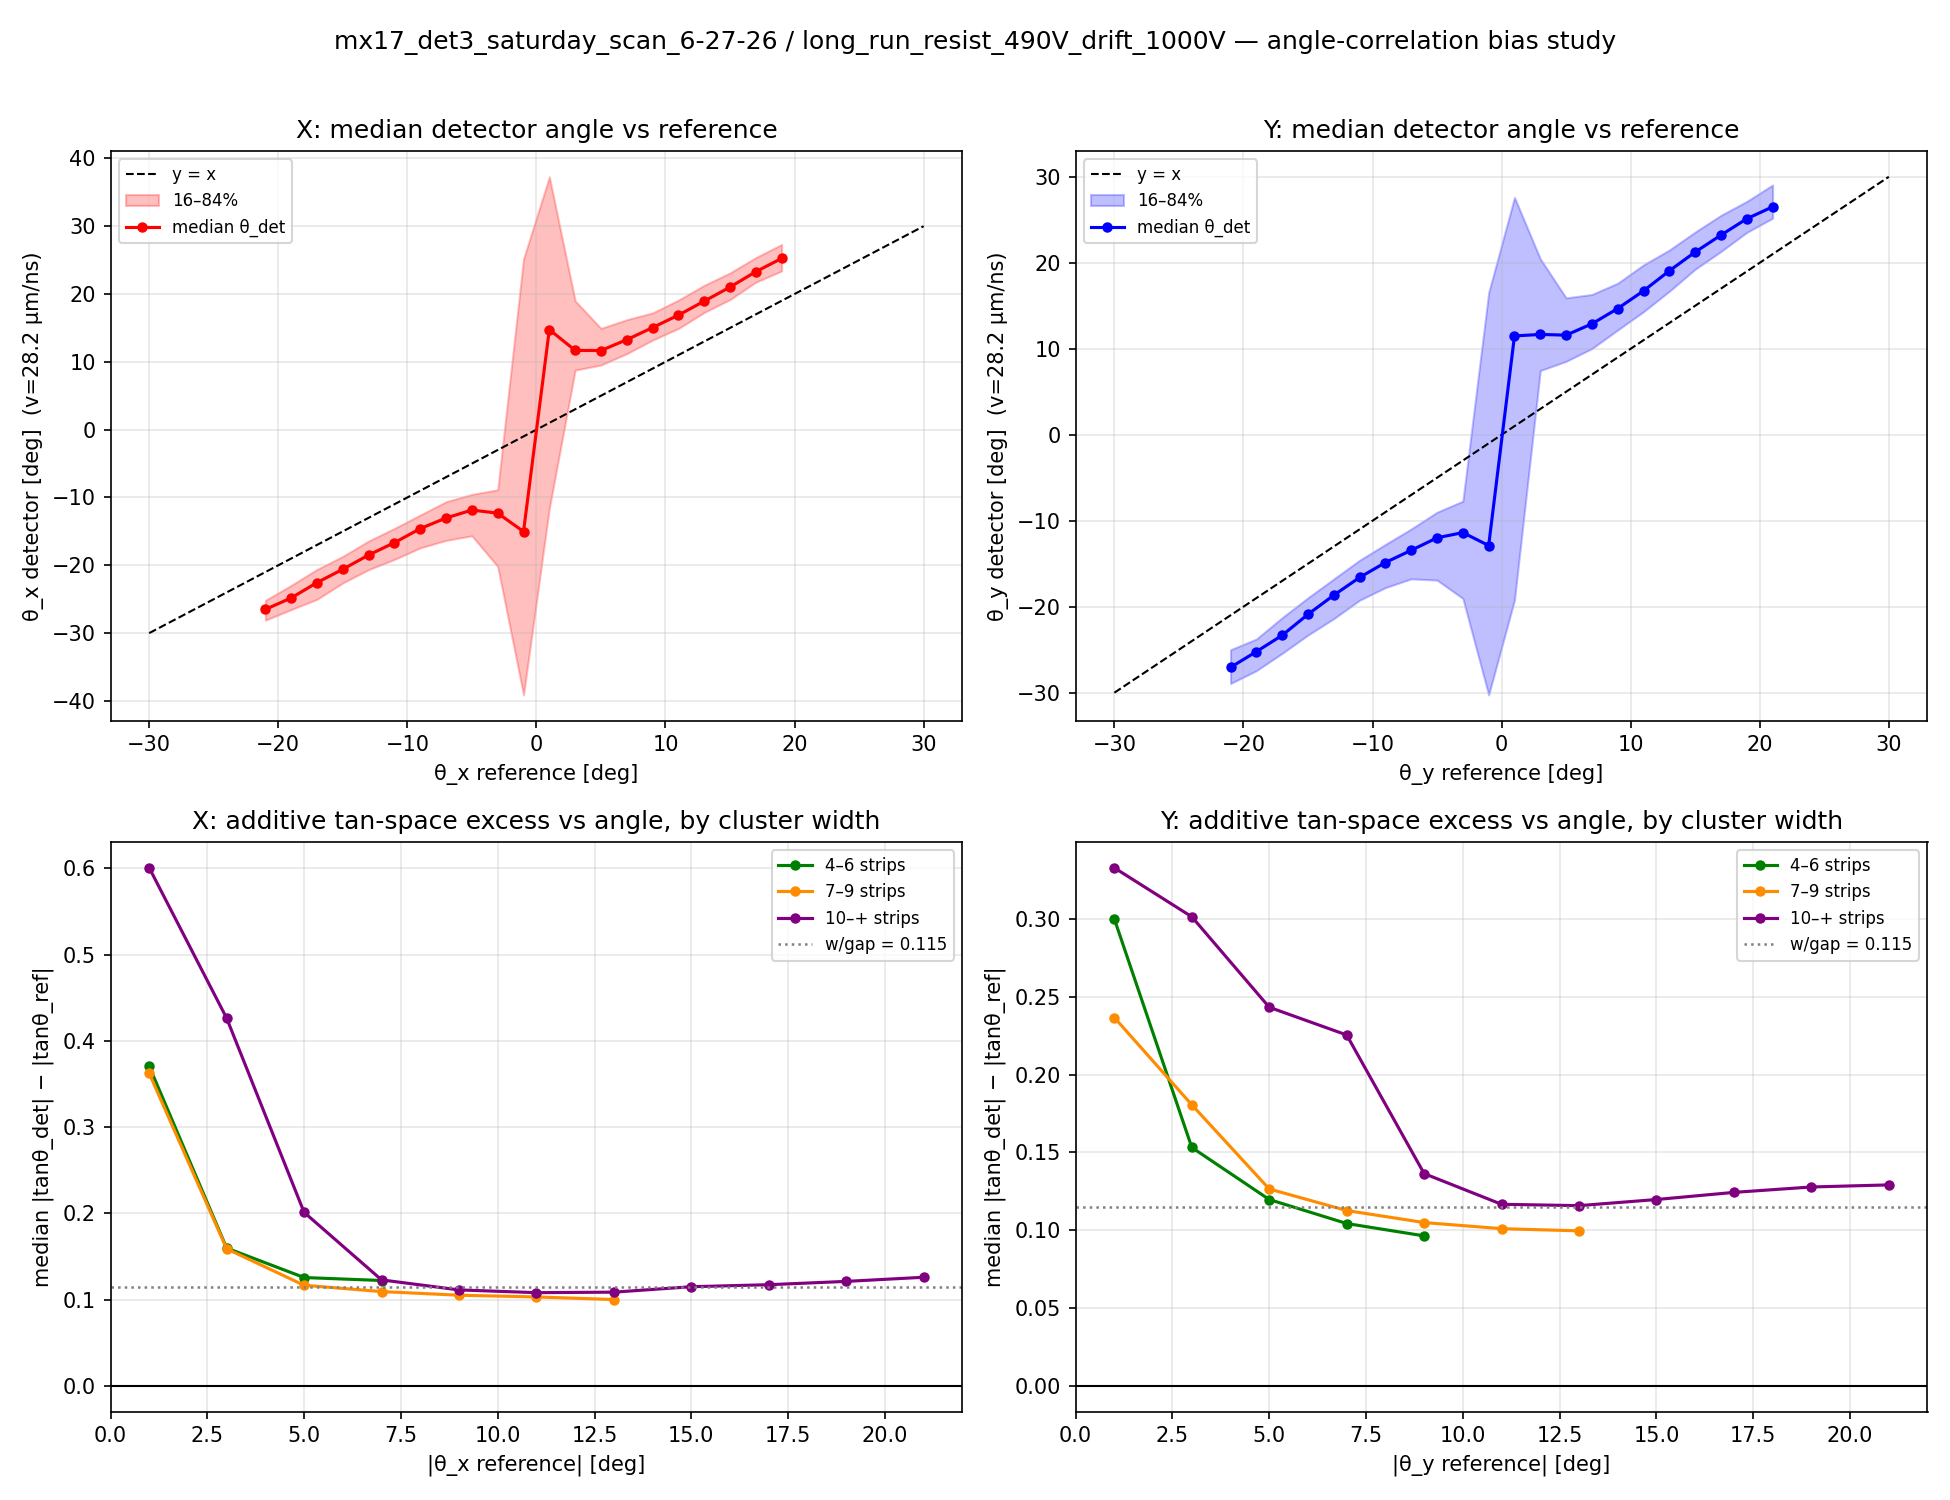
\includegraphics[width=0.9\textwidth]{bias_profiles.png}
\caption{Bias study on the 2.4\,h run. Top: median $\thdet$ vs $\thref$ ---
parallel to the diagonal, displaced outward, with the sign flip through zero.
Bottom: the additive tan-space excess $|\tan\thdet|-|\tan\thref|$ vs
$|\thref|$, split by cluster size; it is flat at $w/z_{\mathrm{rec}}=0.115$ (dotted) above
$\sim\SI{6}{\degree}$ and grows for wide clusters. The rise at small angles is
the $\geq4$-strip selection (only heavily-spread clusters survive).}
\label{fig:biasprofiles}
\end{figure}

\begin{figure}[H]
\centering
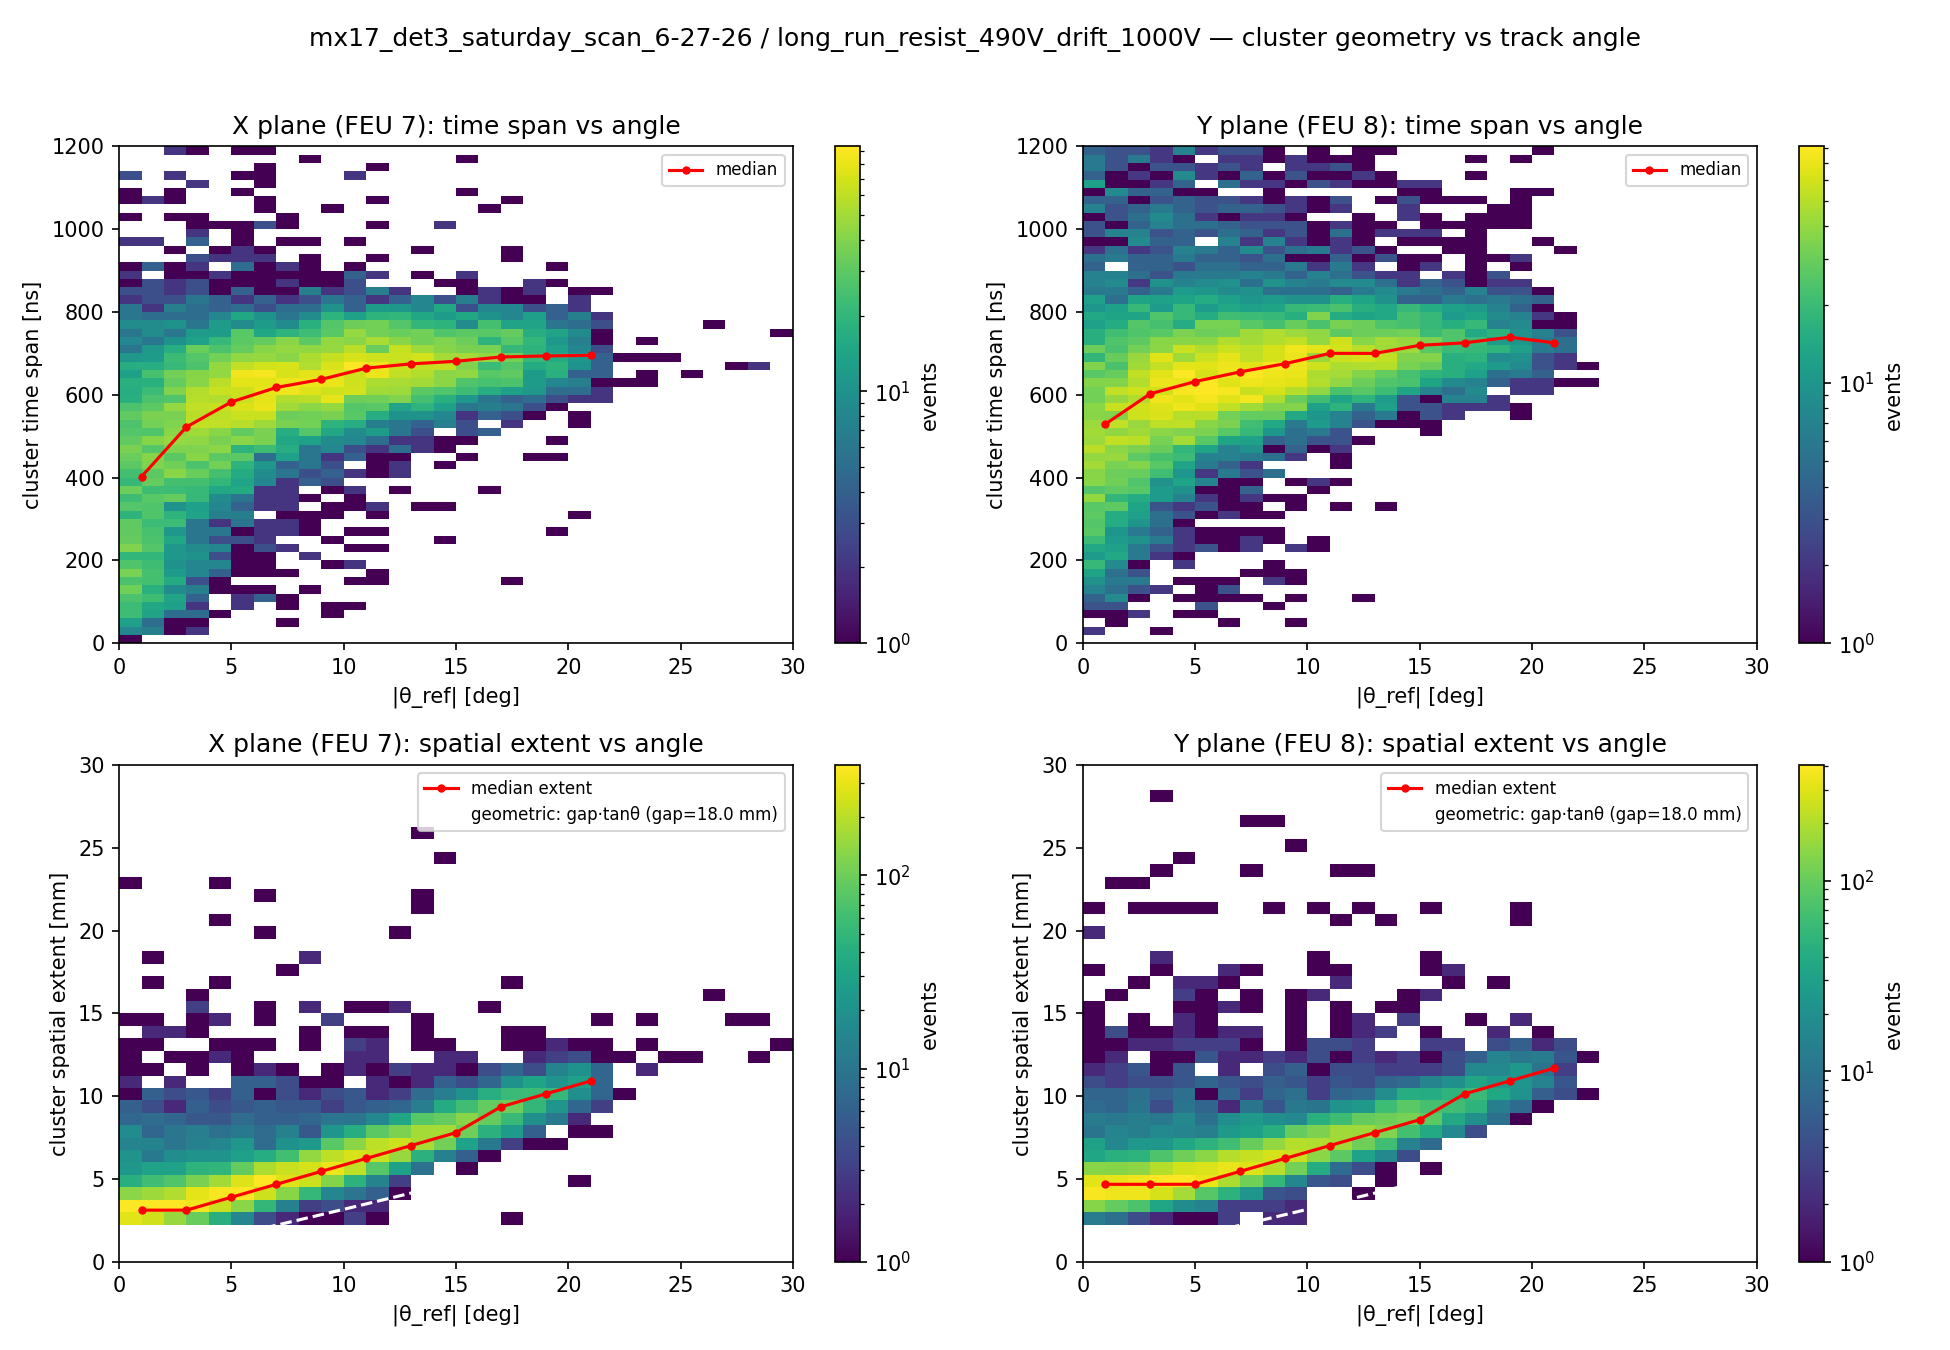
\includegraphics[width=0.9\textwidth]{cluster_geometry.png}
\caption{Cluster geometry vs track angle (2.4\,h run). Top: cluster \emph{time}
span --- saturates at $\Tsat\approx\SI{690}{ns}$ (the drift time across the
visible column) for inclined tracks. Bottom: cluster \emph{spatial} extent ---
a \SIrange{3}{5}{mm} non-geometric floor at $\theta=0$, then growth parallel
to the geometric $z_{\mathrm{rec}}\tan\theta$ (white dashed).}
\label{fig:clustergeom}
\end{figure}

\begin{figure}[H]
\centering
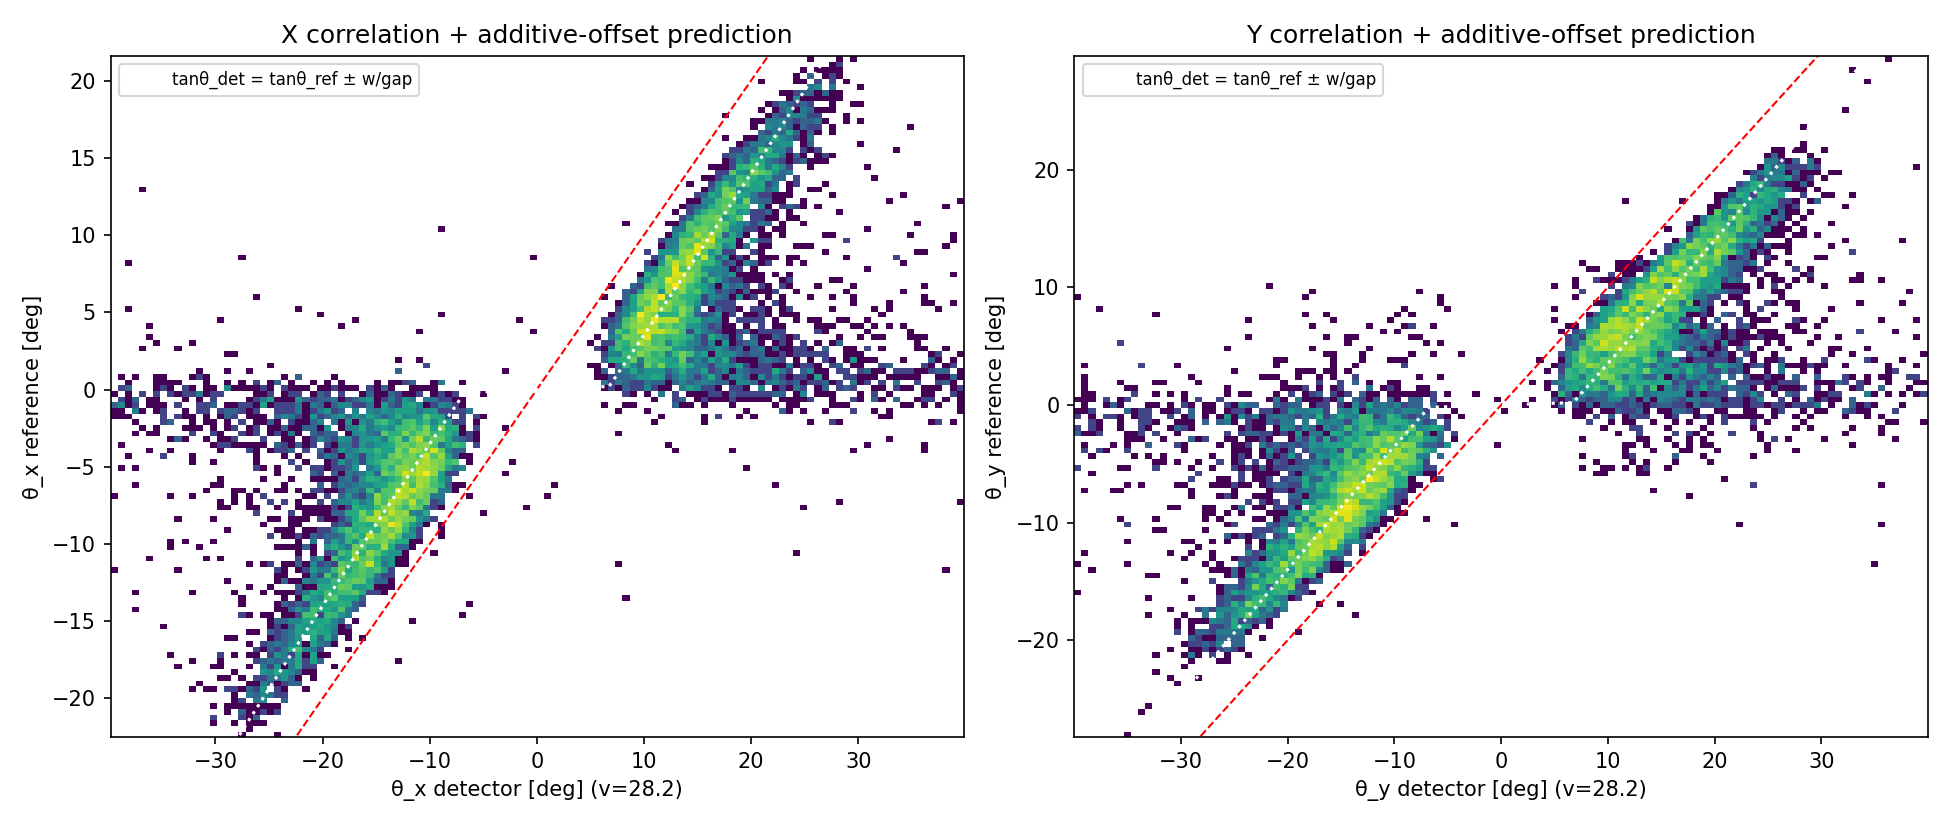
\includegraphics[width=0.94\textwidth]{correlation_with_prediction.png}
\caption{Measured correlation density with the parameter-free prediction of
Eq.~\eqref{eq:offset}, $\tan\thdet = \tan\thref \pm w/z_{\mathrm{rec}}$ (white
dotted), using the independently fitted $w/z_{\mathrm{rec}}=0.115$. The red
dashed line is $y=x$.}
\label{fig:withprediction}
\end{figure}

\subsection{Consequences}

\begin{enumerate}
  \item \textbf{The production $\sigma$-scan drift velocity is biased.}
        The production estimator (Fig.~\ref{fig:sigscan}) scans $\vd$ and
        minimises the width of $|\thref| - |\thdet|$; the additive offset
        pulls its minimum high ($\vd = 30.5/34.0$~\si{\umns} for X/Y on this
        run versus the ridge \SI{28.1}{\umns} --- itself biased low by the
        charge-sharing mechanism of Sec.~\ref{sec:timing}; the physics
        number is the geometric \SI{34}{\umns} of Sec.~\ref{sec:vdrift}).
        Its $|\cdot|$-folding also mixes the sign-following offset into the
        width.  Use the geometry estimator for velocity.
  \item \textbf{A first-order angle correction exists}: subtract
        $\mathrm{sign}(\thdet)\, w/z_{\mathrm{rec}}$ in tan-space.  It sharpens inclined
        tracks but cannot recover $|\theta|\lesssim\SI{5}{\degree}$, where the
        angular information is genuinely destroyed by spreading.
  \item \textbf{Angular resolution} (after slicing in $\thref$, i.e.\ with
        the local bias absorbed): $\sigma_\theta \approx
        \SIrange{1.5}{2}{\degree}$ per plane for
        $|\theta|\gtrsim\SI{5}{\degree}$, degrading to $\sim\SI{6}{\degree}$
        near normal incidence (Fig.~\ref{fig:angres}).
\end{enumerate}

\begin{figure}[H]
\centering
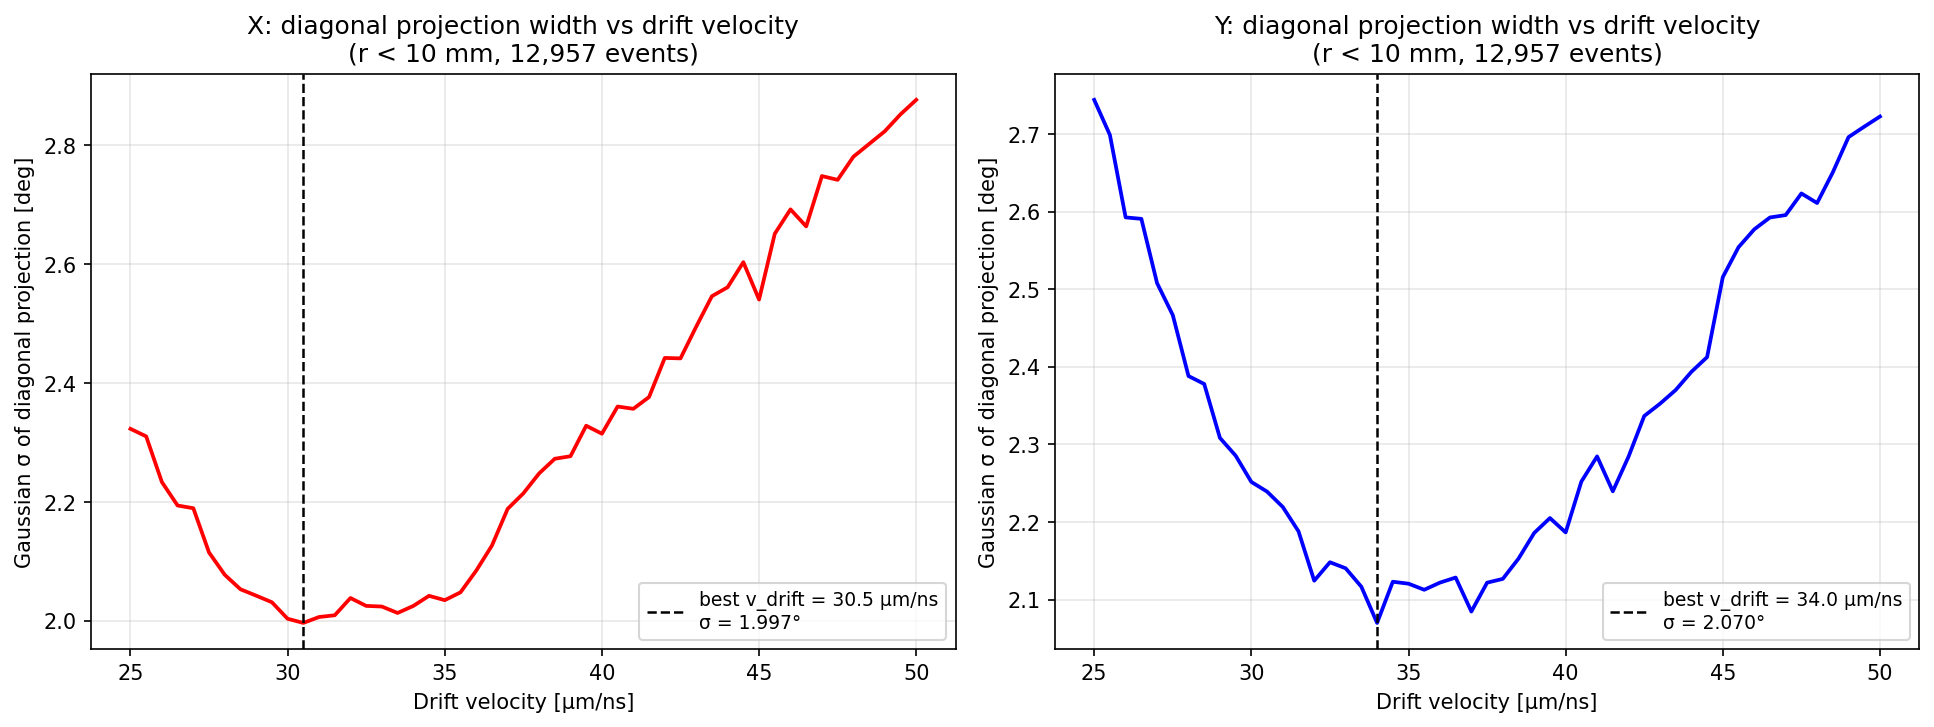
\includegraphics[width=0.9\textwidth]{v_drift_scan.png}
\caption{Production diagonal-projection $\sigma$-scan on the Saturday run.
The minima (X: 30.5, Y: 34.0~\si{\umns}) are biased high by the additive offset;
kept here for reference only.}
\label{fig:sigscan}
\end{figure}

\begin{figure}[H]
\centering
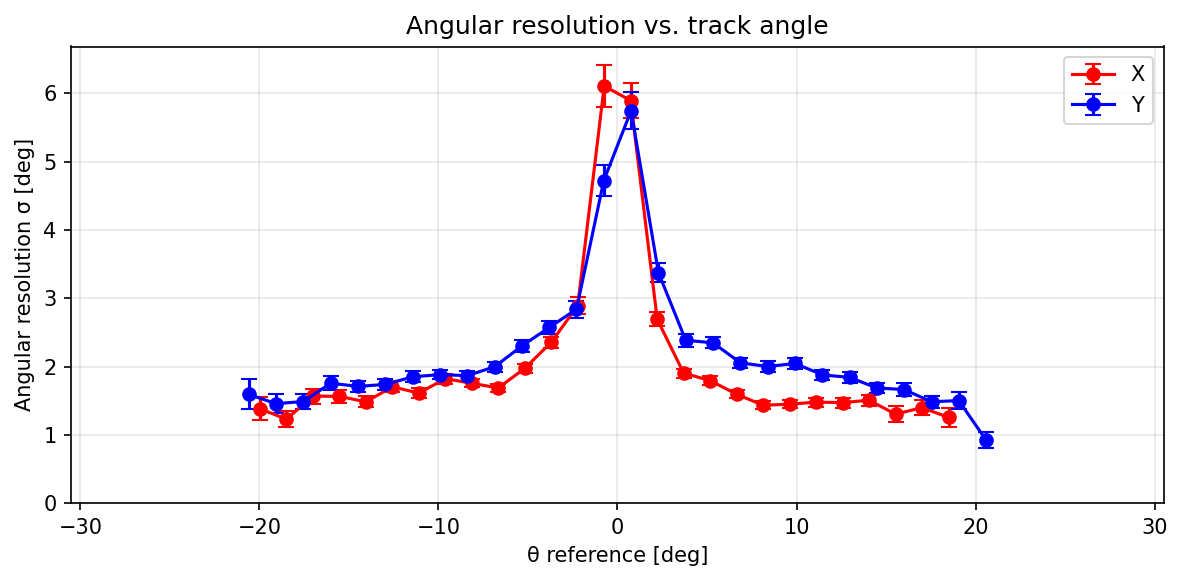
\includegraphics[width=0.78\textwidth]{angular_resolution.png}
\caption{Micro-TPC angular resolution vs track angle (2.4\,h run):
$\sigma_\theta\approx\SIrange{1.5}{2}{\degree}$ per plane for inclined
tracks; the method collapses below $\sim\SI{5}{\degree}$ as predicted by the
spreading mechanism.}
\label{fig:angres}
\end{figure}

%=====================================================================
\section{Drift-velocity measurement from the drift scan}
%=====================================================================
\label{sec:vdrift}

\subsection{First attempt: the ridge fit --- and its hidden assumption}

Rewriting Eq.~\eqref{eq:offset} in terms of the \emph{raw fitted slope}
$S \equiv \vd \tan\thdet$ (in \si{\umns}, after rotation to the M3 frame):
\begin{equation}
  S \;=\; \vd\,\tan\thref \;\pm\; \vd\,\frac{w}{z_{\mathrm{rec}}}.
  \label{eq:ridge}
\end{equation}
If the spreading term is angle-independent, this is a straight line whose
slope is $\vd$ and whose intercept absorbs the offset.  Per-track-sign
straight-line fits (iteratively $3\sigma$-clipped, window
$0.06<|\tan\thref|<0.55$; four independent X/Y~$\times$~sign fits combined)
give the \emph{ridge} velocities of Table~\ref{tab:vdrift} --- at
\SI{1000}{V}, $\SI{28.1\pm0.7}{\umns}$.

The hidden assumption is that $w$ does not depend on angle.  It does: the
ridge is measurably \emph{convex} --- refitting in split windows gives
26--27~\si{\umns} for $|\tan\thref|<0.28$ and 31--32~\si{\umns} for
$|\tan\thref|>0.28$, in both planes, with the intercept simultaneously
shrinking (Fig.~\ref{fig:ridgesys}).  Any angle dependence of the spreading
trades one-for-one into the fitted slope, and a ``flat residual'' check
cannot detect it (a linear $w(\tan\theta)$ is mathematically degenerate with
a change of $\vd$).  The ridge numbers are therefore kept only as the
\emph{time-fit} reference; Sec.~\ref{sec:timing} shows from the raw
waveforms why every time-based fit shares this bias.

\subsection{The geometry estimator}
\label{sec:geomest}

The degeneracy is broken by an observable with \emph{no time axis at all}:
the cluster spatial extent (strip count $\times$ pitch) versus the M3 track
angle.  Its slope is the recorded column depth,
\begin{equation}
  \frac{\mathrm{d}\,\mathrm{extent}}{\mathrm{d}\tan\thref}
     \;=\; z_{\mathrm{rec}} \;+\; w'(\theta),
\end{equation}
with the spreading floor confined to the intercept, and the drift time
across the \emph{same} recorded column is the time-span plateau $\Tsat$.
Their ratio is the drift velocity:
\begin{equation}
  \boxed{\;\vd^{\mathrm{geom}} \;=\;
  \frac{\mathrm{d}\,\mathrm{extent}/\mathrm{d}\tan\thref}{\Tsat}\;}
\end{equation}
Both planes give identical extent slopes (\SI{23.2}{mm} per unit tan on the
2.4\,h run, Fig.~\ref{fig:ridgesys}), beautifully linear over the populated
range, and the estimator is stable when both axes are restricted to the
amplitude \emph{core} of the clusters ($\geq$20/30/40\,\% of the cluster
maximum give $\vd = 35.0\pm0.6$ at \SI{1000}{V};
\texttt{23\_core\_geometry\_vdrift.py}).  The signal-formation closure test
of Sec.~\ref{sec:timing} confirms this estimator recovers the true velocity
within $\sim$3\,\% under data-like conditions, while all time-fit
estimators are biased low.

\begin{figure}[H]
\centering
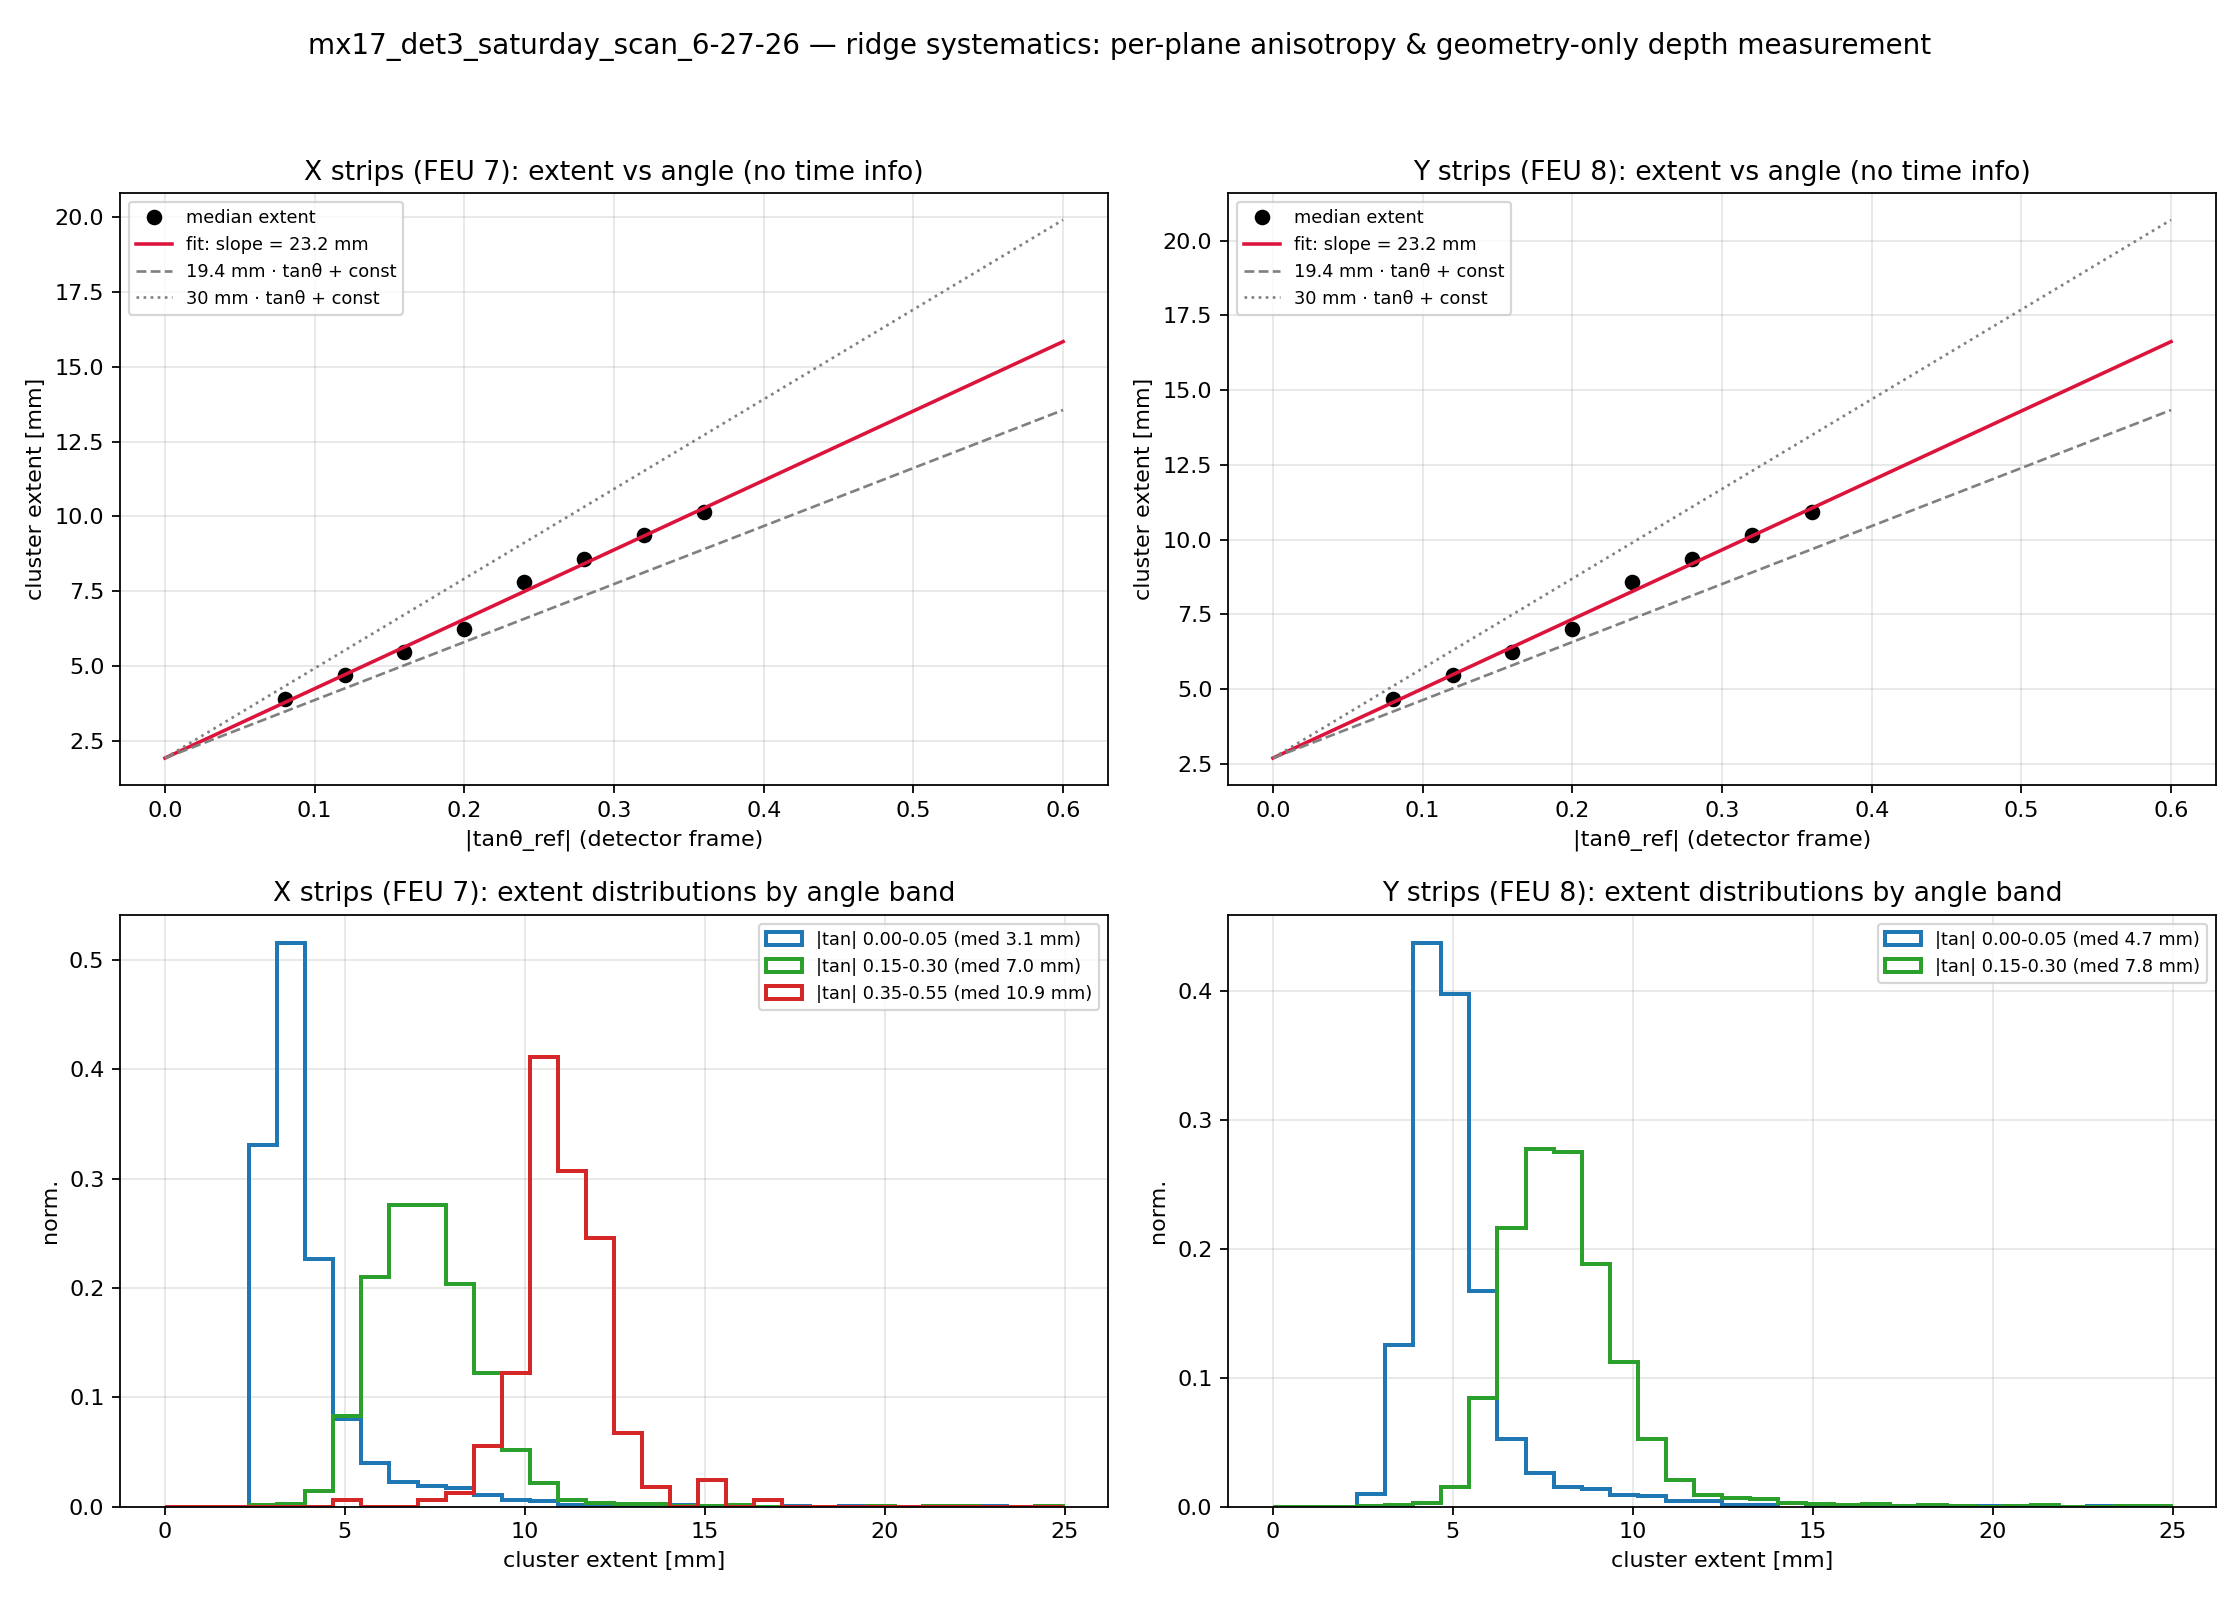
\includegraphics[width=\textwidth]{ridge_systematics.png}
\caption{The geometry measurement (\texttt{20\_ridge\_systematics.py}).
Top: median cluster extent [mm] vs $|\tan\thref|$ (detector frame) --- both
planes give a slope of \SI{23.2}{mm} per unit tan, between the
\SI{19.4}{mm} implied by the (biased) ridge fit and the \SI{30}{mm}
mechanical gap.  Bottom: extent distributions by angle band; the
$\theta\approx0$ floor is \SI{3.1}{mm} (X) / \SI{4.7}{mm} (Y) --- the
anisotropy expected from resistive strips running along $y$.}
\label{fig:ridgesys}
\end{figure}

\subsection{Results}

\begin{table}[H]
\centering
\small\setlength{\tabcolsep}{4.5pt}%
\begin{tabular}{S[table-format=4.0] S[table-format=3.0]
                S[table-format=2.2] @{${}\pm{}$} S[table-format=1.2]
                S[table-format=2.2] @{${}\pm{}$} S[table-format=1.2]
                S[table-format=4.0] l}
\toprule
{drift HV [\si{V}]} & {$E$ [\si{V/cm}]} &
\multicolumn{2}{c}{$\vd$ ridge (biased) [\si{\umns}]} &
\multicolumn{2}{c}{$\vd$ \textbf{geometry} [\si{\umns}]} &
{$\Tsat$ [\si{ns}]} & note \\
\midrule
 100 &  33 & \multicolumn{2}{c}{---} & \multicolumn{2}{c}{---} & {---}
     & drift time $\gg$ window \\
 300 & 100 &  5.70 & 0.54 & \multicolumn{2}{c}{---} & {(1198)}
     & window kills extent lever arm \\
 500 & 167 & 12.77 & 0.43 & 12.37 & 0.39 & {(1361)} & window-truncated column \\
 700 & 233 & 19.45 & 0.53 & 21.61 & 0.53 &  992 & \\
 900 & 300 & 26.17 & 0.84 & 30.03 & 0.64 &  754 & \\
1000 & 333 & 28.12 & 0.65 & 33.91 & 0.25 &  690 & \textbf{2.4\,h long run} \\
1100 & 367 & 29.44 & 0.47 & 35.13 & 0.93 &  661 & \\
\bottomrule
\end{tabular}
\caption{Drift-velocity measurements
(\texttt{14\_drift\_velocity\_scan.py}, \texttt{21\_geometry\_vdrift\_scan.py});
$E = V/\SI{3.0}{cm}$.  The geometry estimator is the physics result; the
ridge column is retained to document the time-fit bias, which grows from
$\approx$0 at \SI{500}{V} to $\approx$20\,\% at \SI{1000}{V}.  Absolute
scale systematic on $\vd^{\mathrm{geom}}$: $\sim$5\,\% (residual spreading
term $w'$, bounded by the core-fraction stability and the toy closure).}
\label{tab:vdrift}
\end{table}

\begin{figure}[H]
\centering
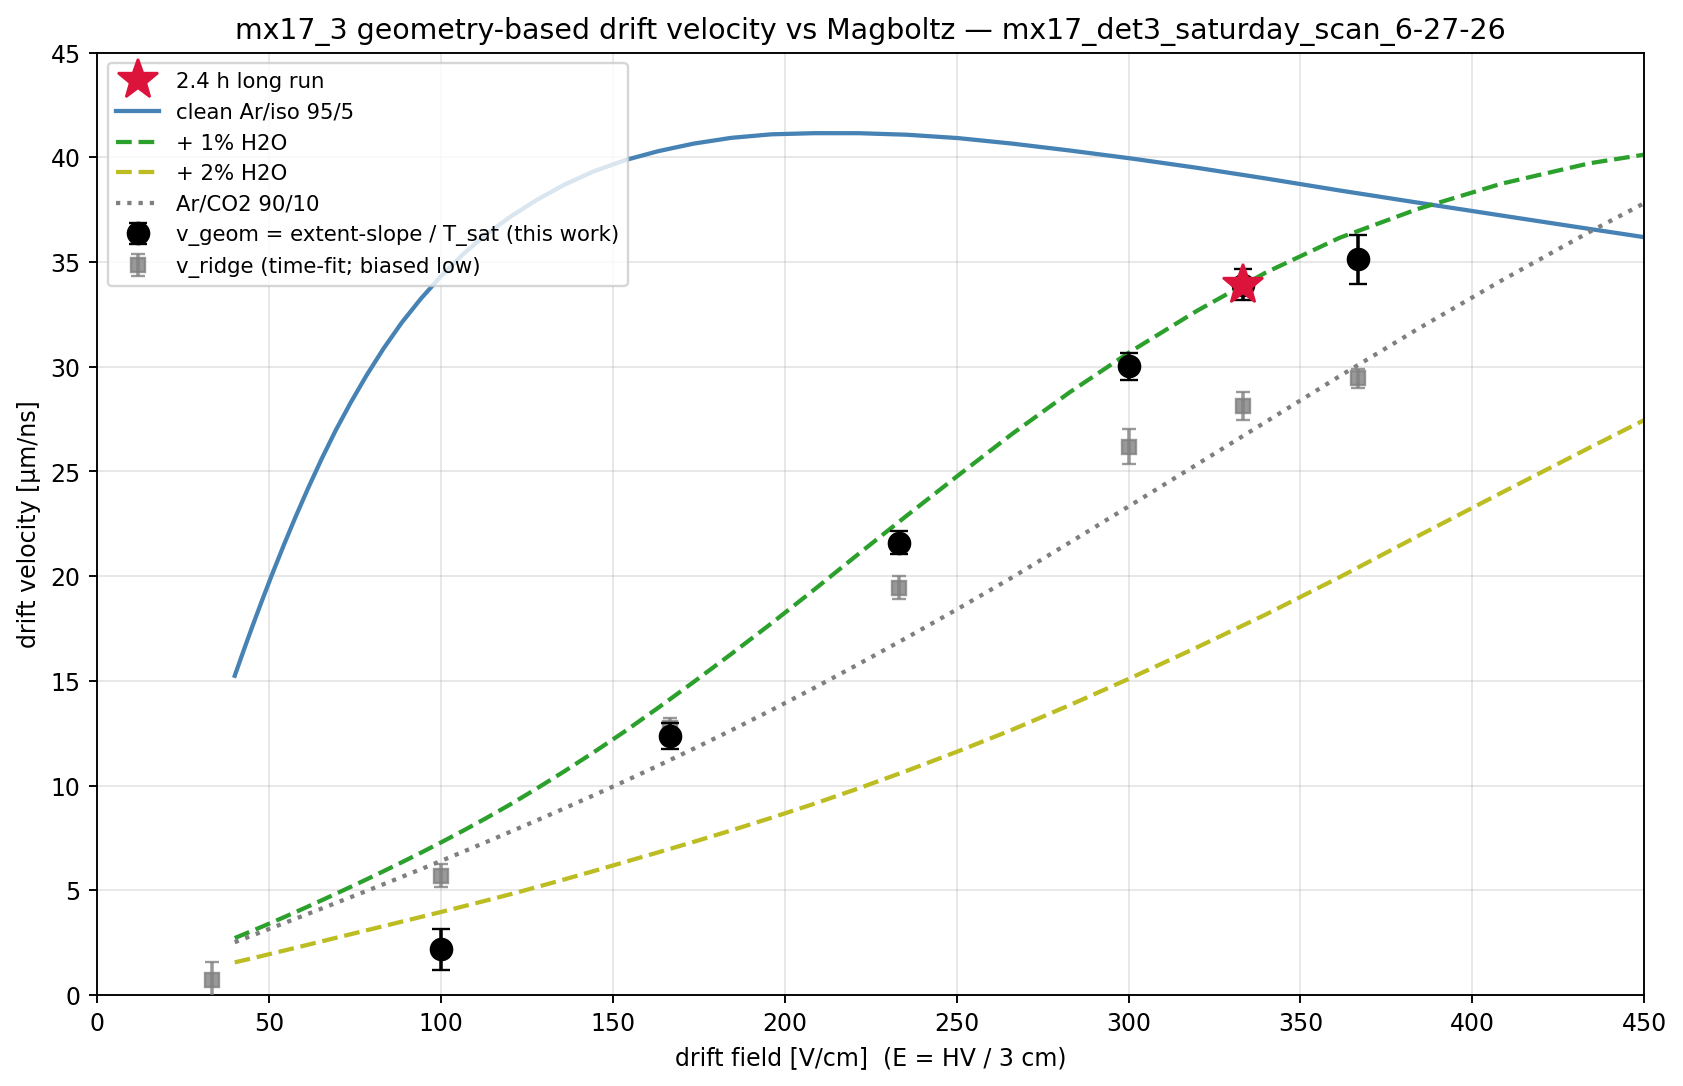
\includegraphics[width=0.82\textwidth]{geometry_vdrift_scan.png}
\caption{Geometry-based $\vd(E)$ (black; star = 2.4\,h run) against the
biased ridge values (grey squares) and Magboltz predictions.  The measured
points thread the Ar/iso 95/5 + \SI{1}{\percent} H$_2$O curve
(Sec.~\ref{sec:gas}).}
\label{fig:vgeomscan}
\end{figure}

Key points:
\begin{itemize}
  \item \textbf{Statistics are not a limitation}: 15-minute scan points give
        \SIrange{1}{3}{\percent} statistical errors.
  \item \textbf{The recorded column is constant}: extent slopes lock at
        \SIrange{21}{23.5}{mm} for $\geq\SI{700}{V}$ (Sec.~\ref{sec:gap}).
  \item \textbf{The low-HV points die by window truncation}: at
        \SIrange{100}{300}{V} most charge arrives after the
        \SI{1.92}{\micro s} DREAM window closes; the same truncation
        (plus stronger low-field attachment) drives the efficiency turn-on
        of the drift scan (Fig.~\ref{fig:driftscaneff}): \SI{44}{\percent}
        at \SI{100}{V} rising to \SI{83}{\percent} at $\geq\SI{700}{V}$ ---
        the quantitative version of ``det3 needs drift $\geq\SI{700}{V}$''.
\end{itemize}

\begin{figure}[H]
\centering
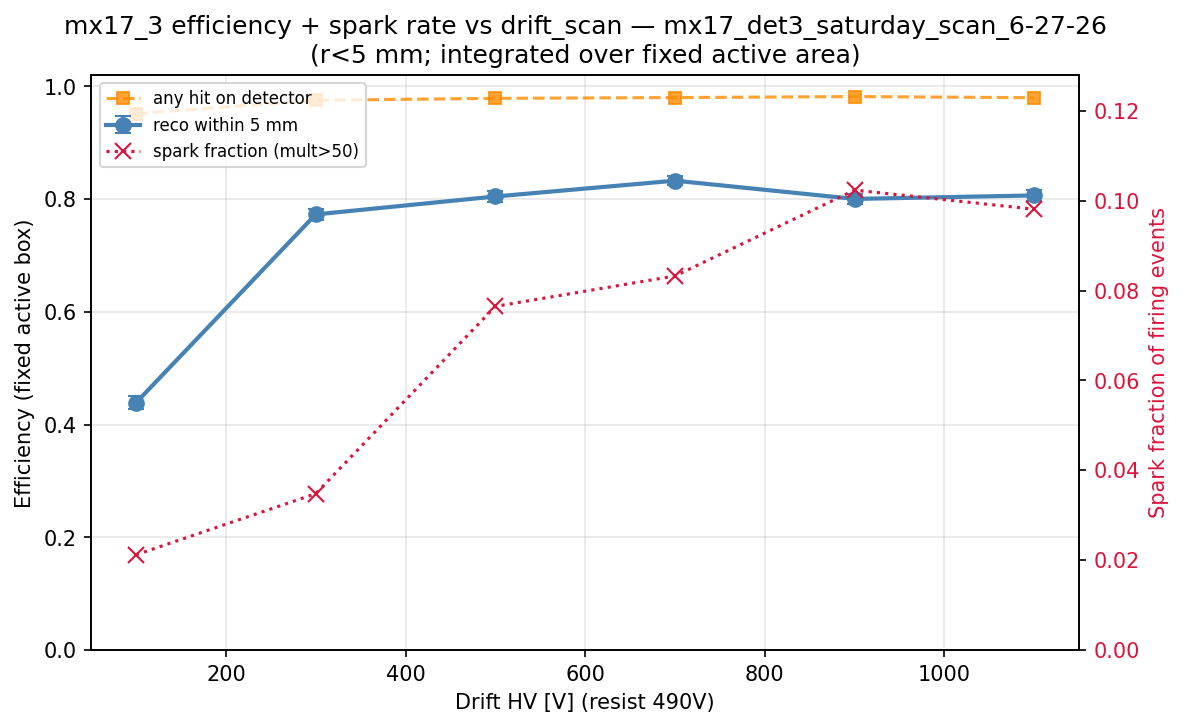
\includegraphics[width=0.62\textwidth]{efficiency_vs_drift_scan.png}
\caption{Reconstruction efficiency vs drift HV (drift scan, fixed active
box).  The turn-on tracks the fraction of the drift column whose charge
arrives inside the readout window (and survives attachment); the plateau
begins once the surviving column's drift time fits in the window.}
\label{fig:driftscaneff}
\end{figure}

%=====================================================================
\section{Why every time-based fit is biased: waveforms, charge sharing,
         and a simulation closure}
%=====================================================================
\label{sec:timing}

The 20\,\% gap between the ridge and geometry velocities demands an
explanation at the signal level.  The decoded (non-zero-suppressed) DREAM
data of the long run --- 512 channels $\times$ 32 samples per event and FEU
--- were pulled from the lxplus archive and analysed strip by strip
(\texttt{24\_waveform\_investigation.py}).

\subsection{What the waveforms show}

\begin{figure}[H]
\centering
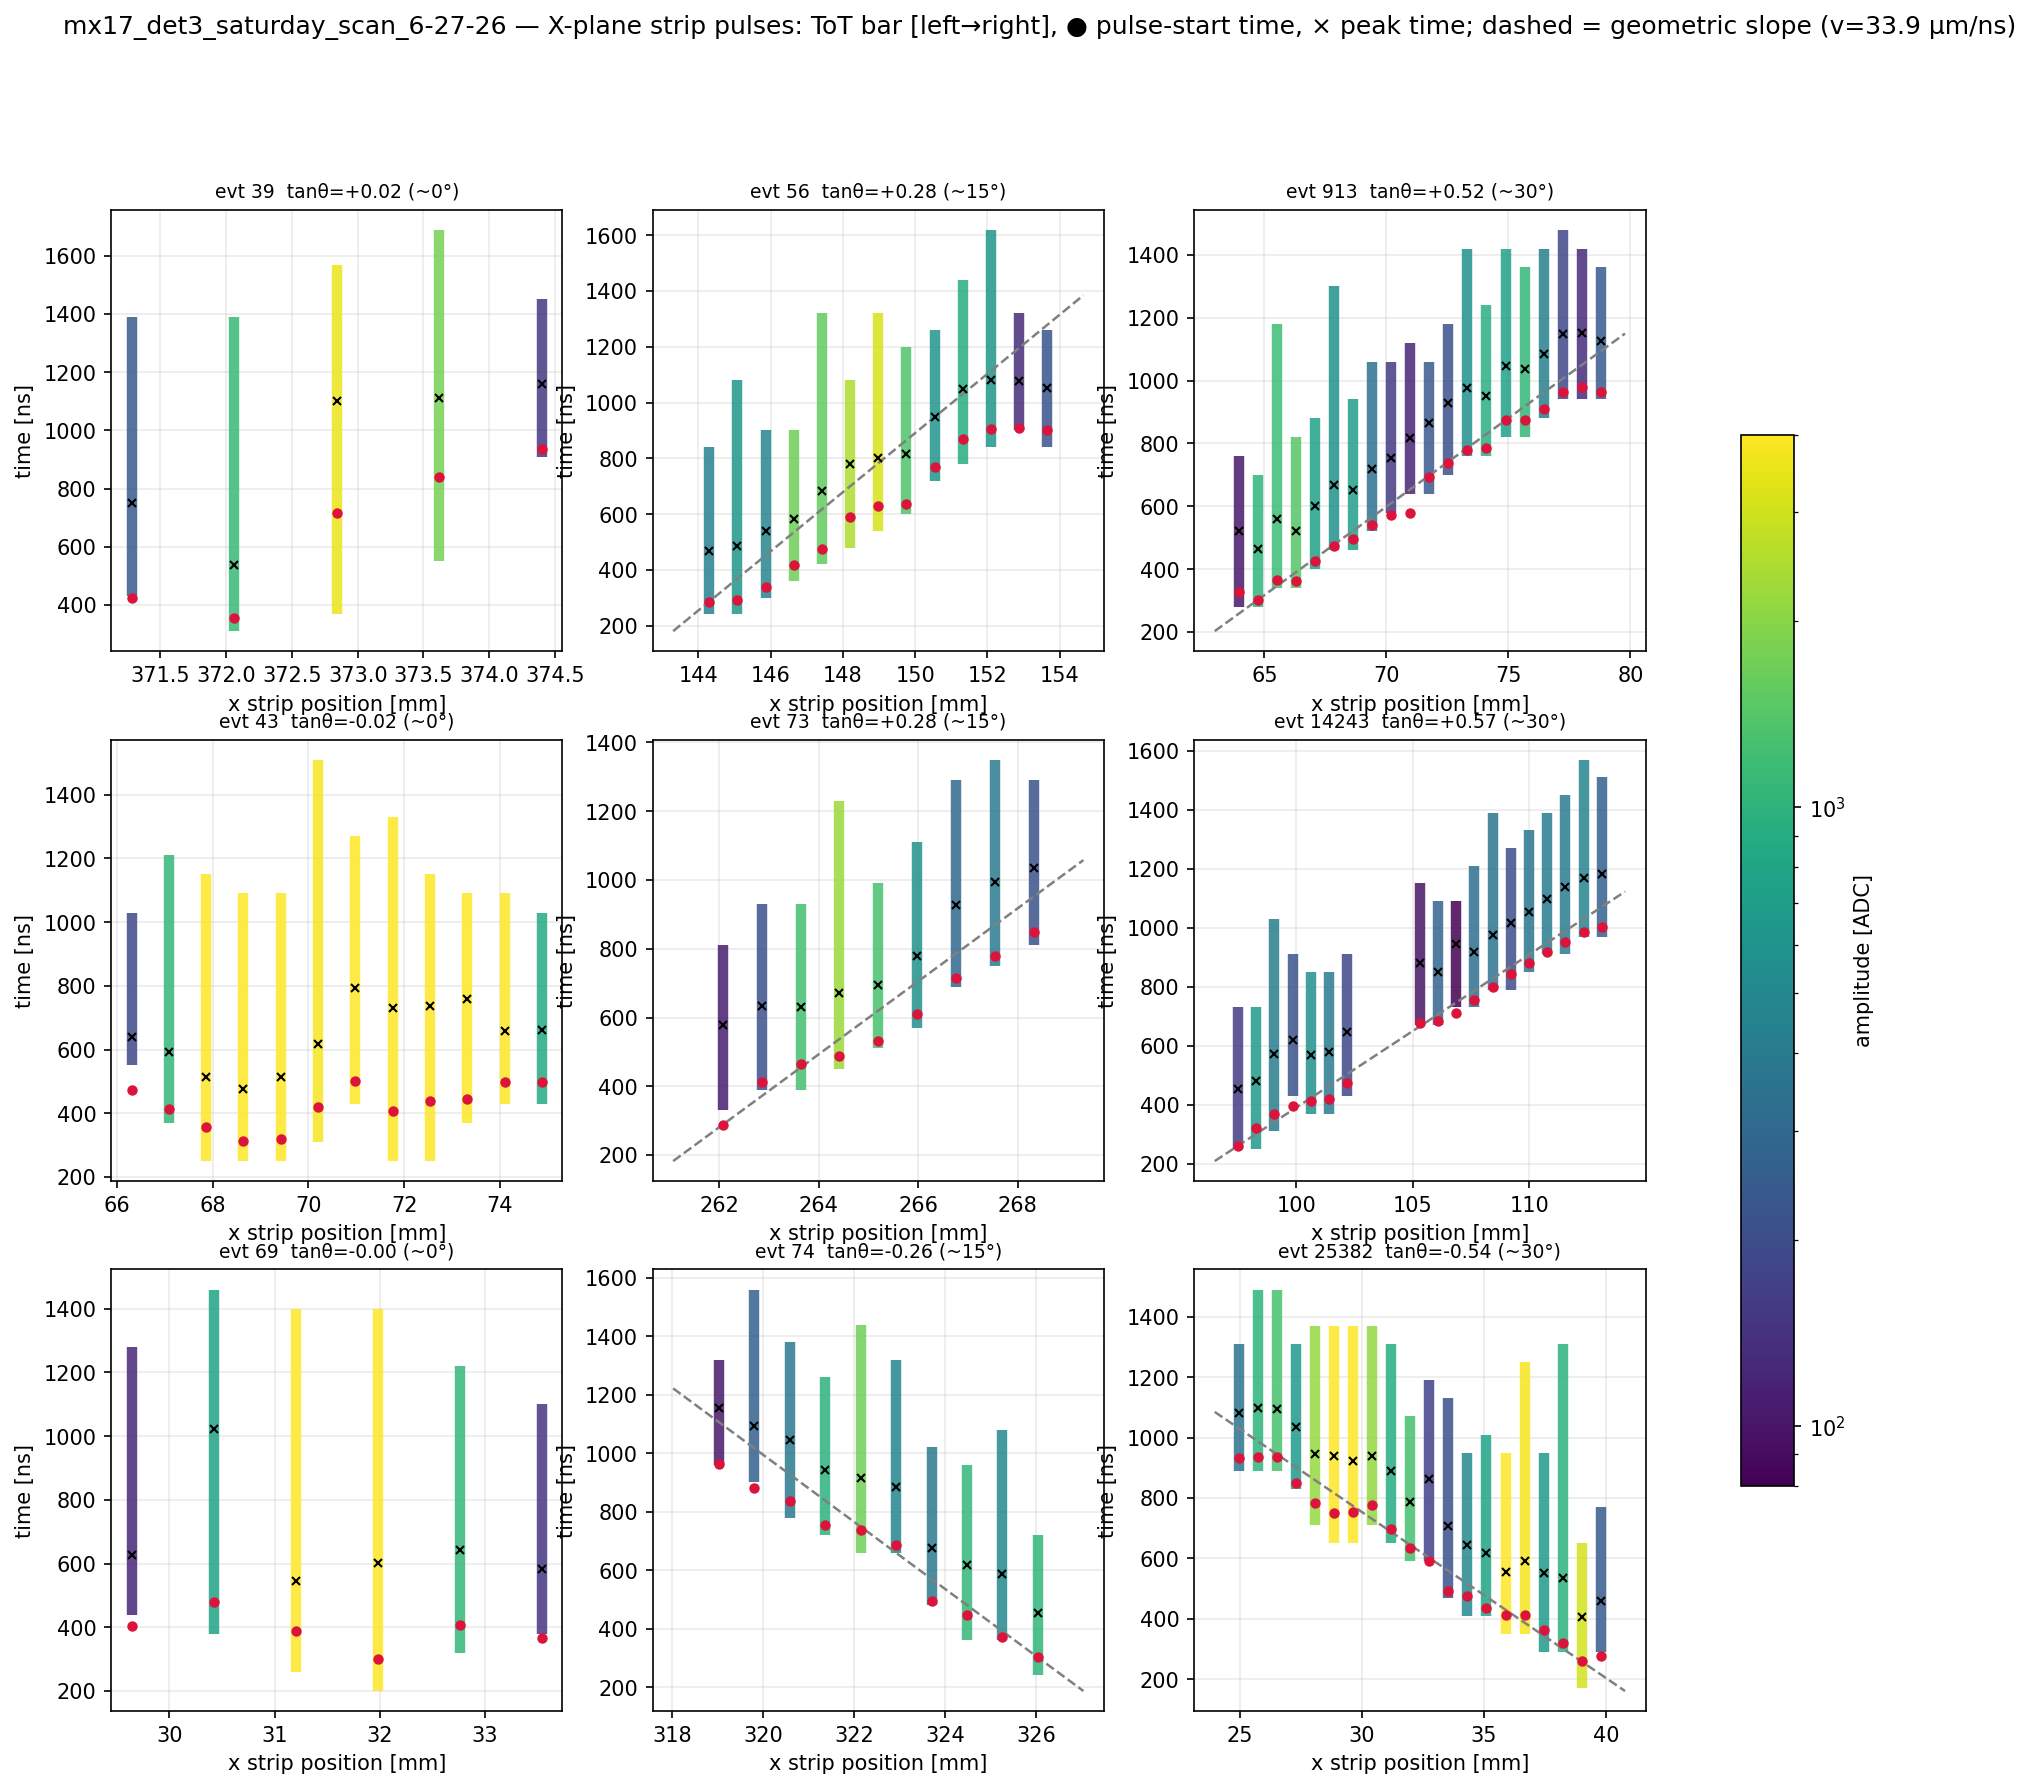
\includegraphics[width=\textwidth]{strip_timing_displays.png}
\caption{Per-strip pulse structure for reference tracks at
$\sim$0/15/30$^\circ$ (columns): time-over-threshold bars vs strip position,
colour = amplitude; $\bullet$ = pulse-start time, $\times$ = peak time;
dashed = the geometric slope at $\vd^{\mathrm{geom}}$.  The time ladder
follows geometry through the cluster core but \emph{flattens at both ends}:
low-amplitude mesh-end strips start late, deep-end strips fire early.}
\label{fig:wfdisplays}
\end{figure}

Three facts, from Figs.~\ref{fig:wfdisplays} and \ref{fig:wfshapes}:
\begin{enumerate}
  \item \textbf{The hit times are faithful to the waveforms.}  Re-deriving
        each strip's time from the raw samples with four independent
        estimators --- fixed threshold, constant-fraction (50\,\%),
        rising-edge fit, derivative maximum --- and refitting the track
        slope on core strips gives $\vd = $ 28.0--30.5~\si{\umns}: the same
        as the production pulse fit.  The bias is \emph{not} in the pulse
        fitting.
  \item \textbf{The pulse shapes are healthy}: the rise scale
        ($t_{\mathrm{peak}}-t_{\mathrm{CFD}}$) is $\approx\SI{140}{ns}$ for
        every amplitude class (the shaper), and core-strip time residuals
        from the track line show no amplitude walk.  Skirt strips carry
        late tails of \SIrange{+200}{+400}{ns}.
  \item \textbf{The ladder, not the pulses, is distorted}: within one
        cluster the time--position relation is S-shaped --- geometric in
        the middle, flattened at both ends --- so a straight-line fit
        returns a slope steeper (in ns/mm) than geometry, i.e.\ a velocity
        that is too low, while the endpoints span less time than the
        geometric column implies.
\end{enumerate}

\begin{figure}[H]
\centering
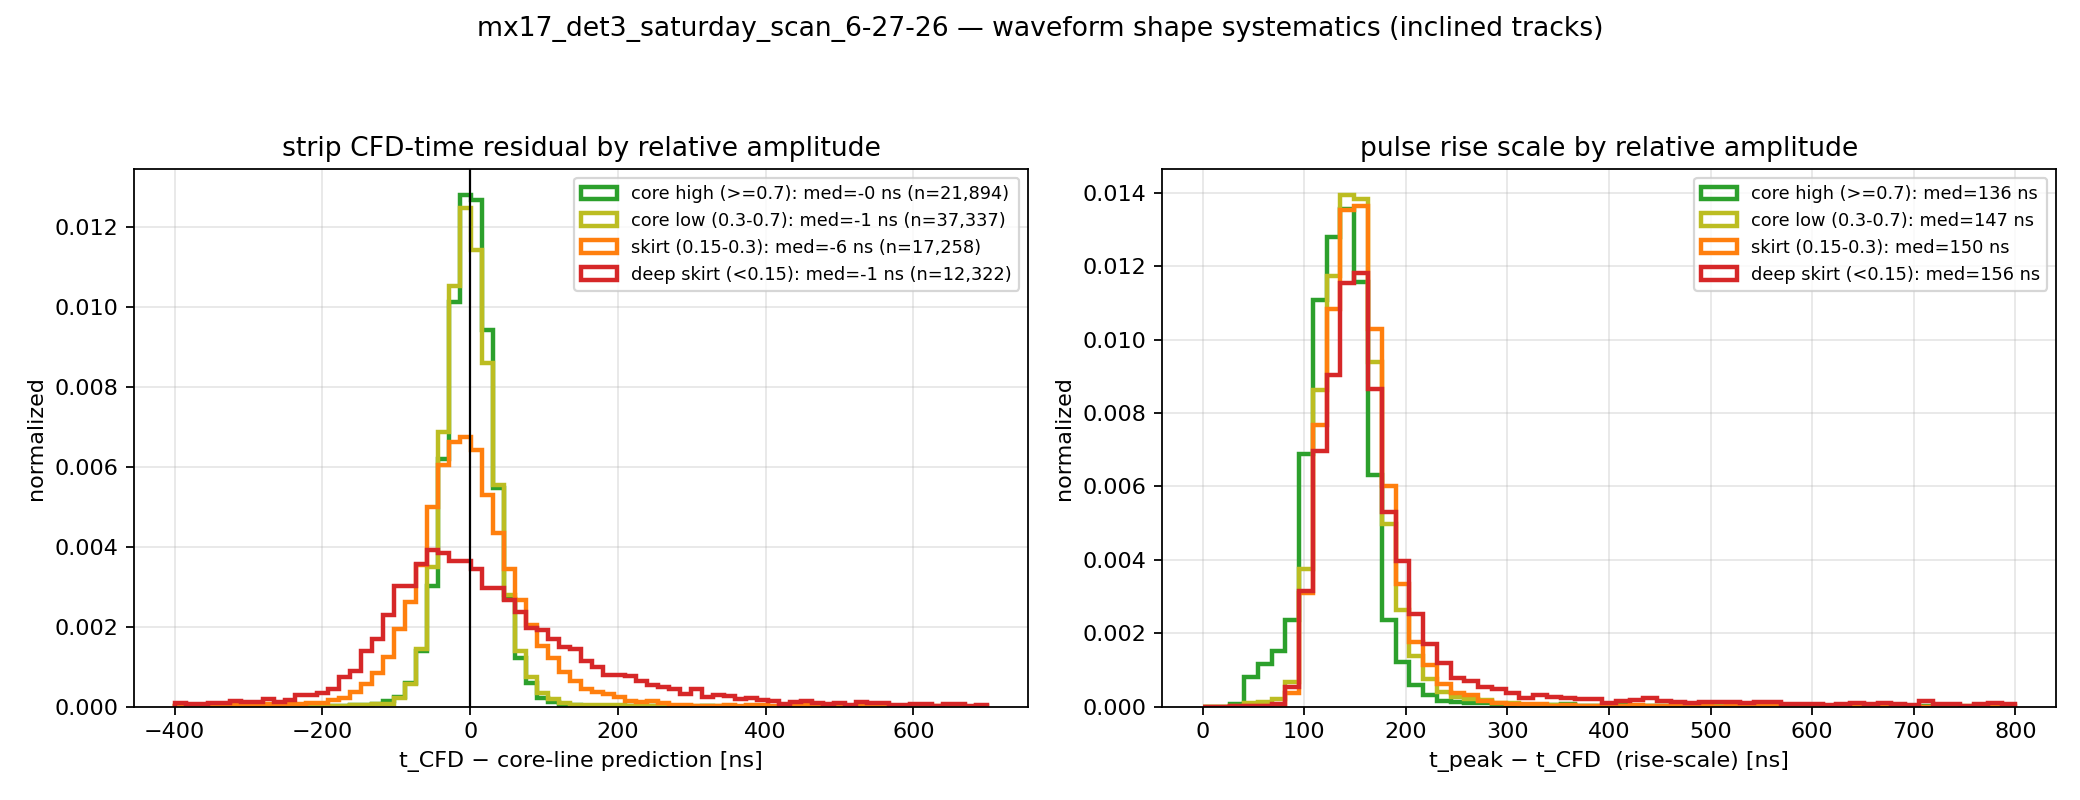
\includegraphics[width=\textwidth]{wf_shapes.png}
\caption{Waveform shape systematics (inclined tracks).  Left: CFD-time
residual from the core line by relative amplitude --- core strips are tight
and unbiased; skirt strips have heavy late tails.  Right: rise scale is
$\approx\SI{140}{ns}$ for all classes --- pulse shapes are not the problem.}
\label{fig:wfshapes}
\end{figure}

\subsection{The mechanism: prompt charge sharing}

On a resistive-strip anode a substantial fraction of every strip's charge
appears (almost) promptly on its neighbours --- capacitive coupling plus
dispersion; the along-$y$ RC component additionally widens the
$y$-measurement footprint (the \SI{4.7}{mm} vs \SI{3.1}{mm} floors of
Fig.~\ref{fig:ridgesys}).  Figure~\ref{fig:sharingdiag} illustrates the
chain of consequences.  For an inclined track each strip's waveform is a
superposition of its own (direct) charge and \emph{earlier} charge shared
from its shallower neighbour (panel b): the pulse start is pulled early or
late depending on the local amplitude balance.  Where direct charge is
strong (core middle) the distortion is small; at the deep end, where
attachment has weakened the direct charge, the shared component dominates
and the strip fires at nearly its neighbour's time.  The time--position
ladder is therefore S-shaped (panel c): geometric in the middle, flattened
at both ends --- and any straight-line fit through it returns a slope that
is too steep in ns/mm, i.e.\ a velocity that is too low.  Note the trap:
because \emph{all} per-strip times inherit this distortion, re-deriving
them from the raw waveforms with better pulse estimators changes nothing
--- the bias is in the physics of the signal, not in the fitting.

\begin{figure}[H]
\centering
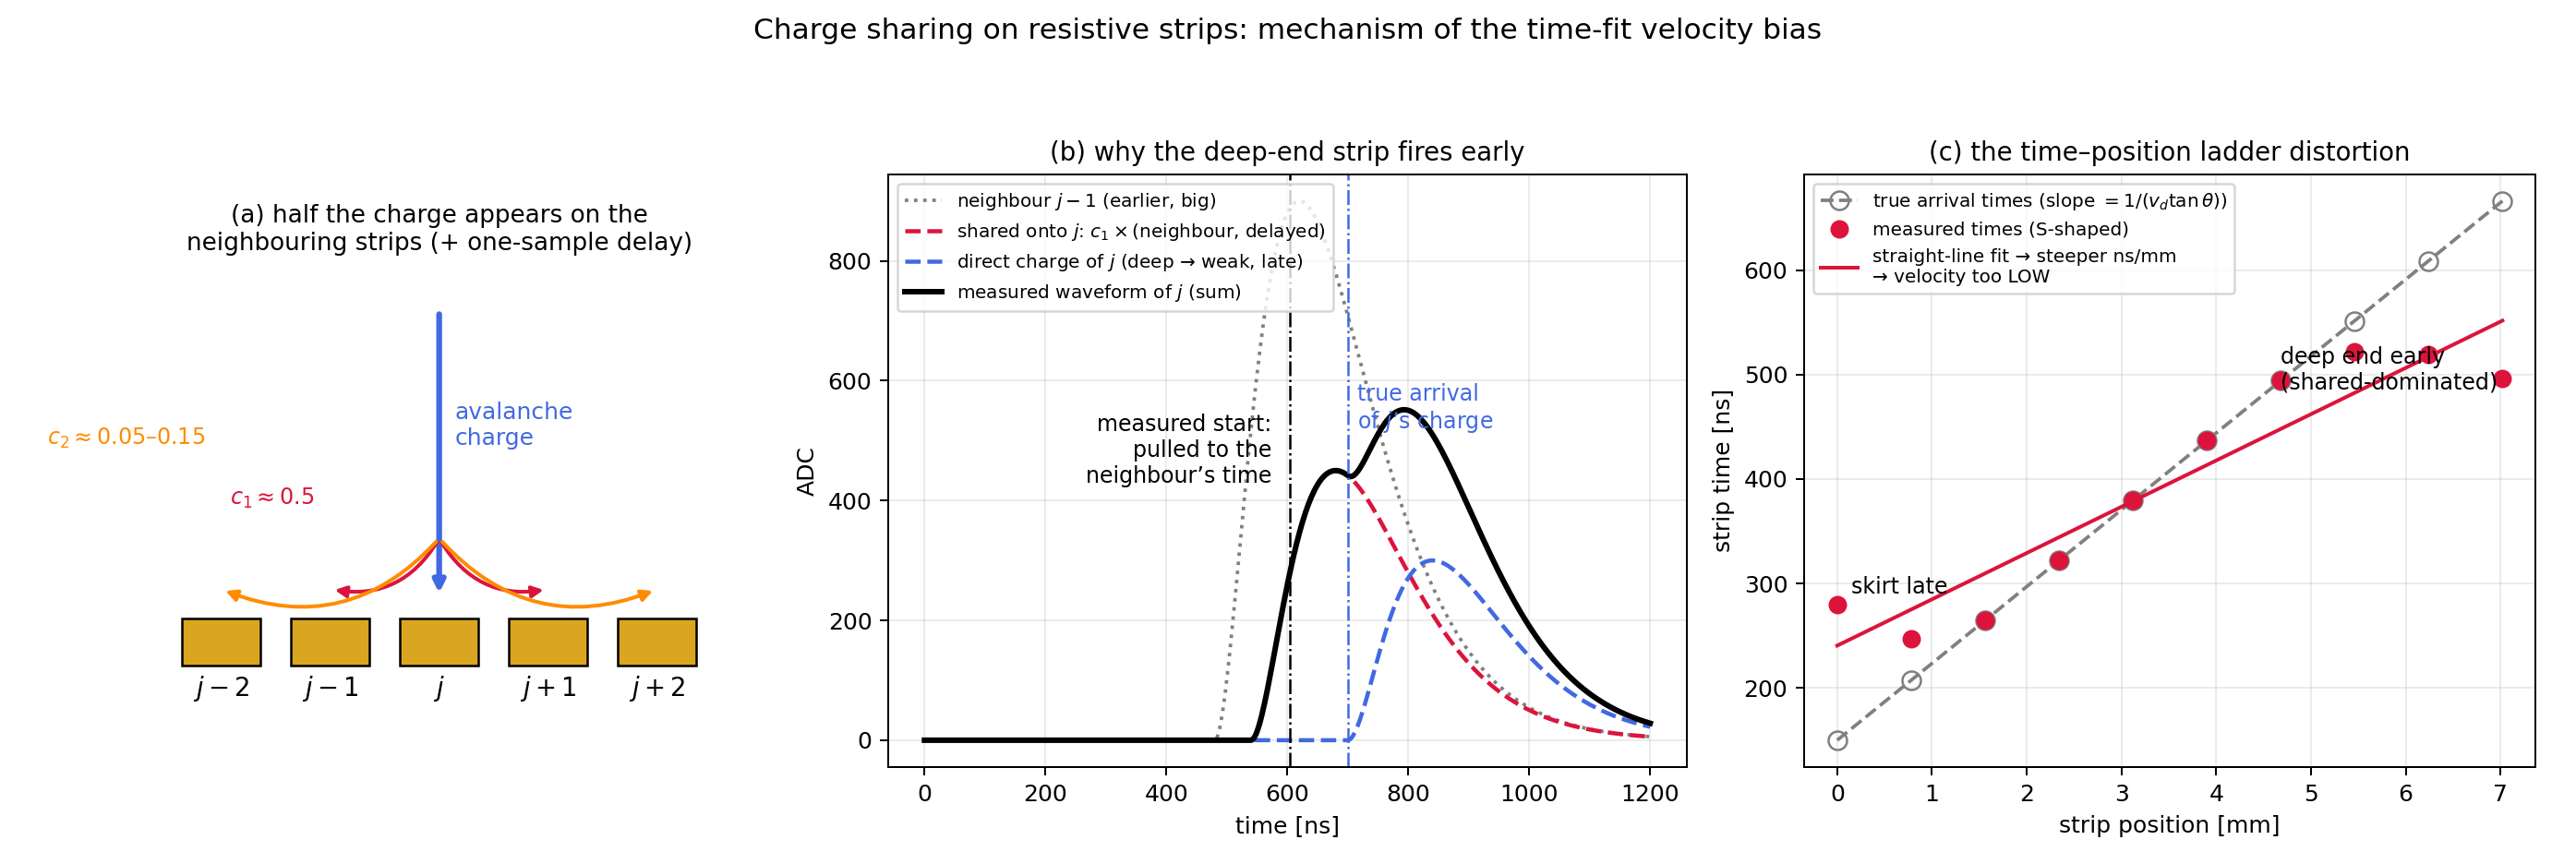
\includegraphics[width=\textwidth]{diagram_sharing.png}
\caption{The charge-sharing mechanism, schematically.  (a) The avalanche
charge of one strip appears at $c_1\approx0.5$ on each first neighbour and
$c_2\approx0.05$--$0.15$ on each second neighbour, with a one-sample
($\approx\SI{60}{ns}$) delay.  (b) A weak (deep-end) strip's measured
waveform is dominated by the shared copy of its earlier neighbour; its
fitted start time is pulled to the neighbour's time.  (c) The resulting
S-shaped time--position ladder: a straight-line fit is steeper (ns/mm)
than the true drift relation, biasing the velocity low.}
\label{fig:sharingdiag}
\end{figure}

\subsection{Closure test with a signal-formation toy MC}

A toy simulation (\texttt{25\_signal\_formation\_toy.py}) generates
waveform-level events with known $\vd^{\mathrm{true}}$: ionisation clusters
along the track, exponential gain fluctuations, attachment, transverse and
longitudinal diffusion, prompt charge sharing to $\pm1/\pm2$ neighbours,
CR--RC$^2$ shaping (peak \SI{140}{ns}), \SI{60}{ns} sampling, noise and
thresholds --- then runs the \emph{same} estimators as on data.  With
sharing fractions of $\sim$35\,\%/12\,\% and
$\lambda_{\mathrm{att}}\approx\SI{10}{mm}$ the toy reproduces the data
pattern simultaneously: extent slope \SI{23.6}{mm} (data 23.2),
$\Tsat = \SI{695}{ns}$ (data 690), extent floor \SI{4.7}{mm}, and time-fit
velocities 15--25\,\% below truth.  Scanning $\vd^{\mathrm{true}}$ at fixed
parameters:
\begin{itemize}
  \item the \textbf{geometry estimator recovers $\vd^{\mathrm{true}}$ within
        $\sim$3\,\%} at every velocity tested (28--37~\si{\umns});
  \item every \textbf{time-fit estimator is biased low}, by an amount that
        matches the data hierarchy (production anchored/weighted worst,
        CFD-core best);
  \item $\Tsat$ pins the velocity independently: \SI{690}{ns} is reproduced
        only for $\vd^{\mathrm{true}} \approx \SI{34}{\umns}$.
\end{itemize}

\noindent\textbf{Conclusion:}
\begin{equation}
  \boxed{\;\vd(\SI{1000}{V}) \;=\; \SI{34 \pm 1.5}{\umns}\;}
\end{equation}
with the geometry estimator validated as unbiased, and all time-based fits
(production and waveform-level alike) low by 10--20\,\% through prompt
charge sharing.

\subsection{The fix, prototyped on data: waveform unsharing}
\label{sec:unsharing}

The correction is a linear deconvolution across strips applied to the
waveforms \emph{before} timing: solve
$(\mathbb{1} + c_1 E_{\pm1} + c_2 E_{\pm2})\,\mathbf{w}' = \mathbf{w}$
per time sample (a banded system; $E_{\pm k}$ shifts by $k$ strips).  On
the toy MC with known sharing this restores the time-fit velocity from
27.4 to 33.1 for $\vd^{\mathrm{true}}=34$.  On data
(\texttt{26\_unsharing\_analysis.py}):
\begin{itemize}
  \item the sharing fractions are \emph{measured} from near-vertical tracks
        (neighbour/lead amplitude ratios; Fig.~\ref{fig:unsharing}):
        $c_1 = 0.45/0.52$, $c_2 = 0.05/0.15$ for the $x$/$y$ planes ---
        about half of each strip's charge appears on its neighbours, more
        second-neighbour reach in $y$ (the along-strip RC direction) ---
        with a $+\SI{69}{ns}$ (one-sample) median neighbour delay;
  \item after unsharing and re-timing, the CFD core-line ridge gives
        $\vd = \SI{33.8\pm0.6}{\umns}$ ($x$) and $\SI{32.9\pm0.3}{\umns}$
        ($y$) --- \textbf{in agreement with the geometry estimator's
        \SI{33.9}{\umns}}.  Time-based and geometric velocity measurements,
        biased apart by 20\,\% before the correction, converge.
\end{itemize}
The sharing constants are measured from amplitude ratios only --- no
velocity information enters --- so this is an independent confirmation of
$\vd$, and a demonstration that the correction is feasible offline on the
existing (frozen) dataset.  Promoting it to the production hit converter
(with a one-sample delay kernel for the $y$ plane as a refinement) is the
concrete path to unbiased micro-TPC angles.

\begin{figure}[H]
\centering
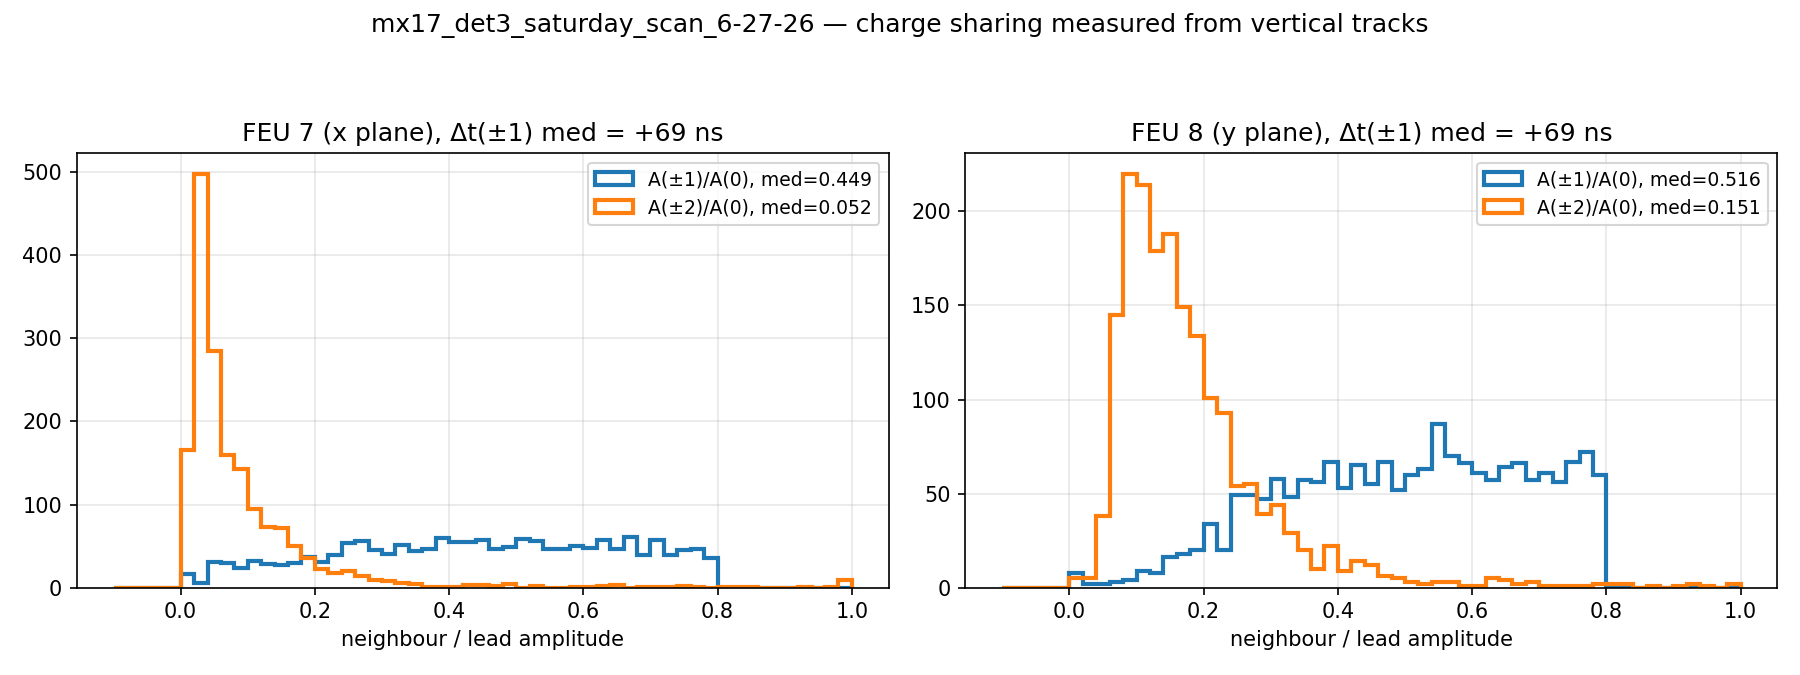
\includegraphics[width=0.9\textwidth]{unsharing_sharing.png}\\[1mm]
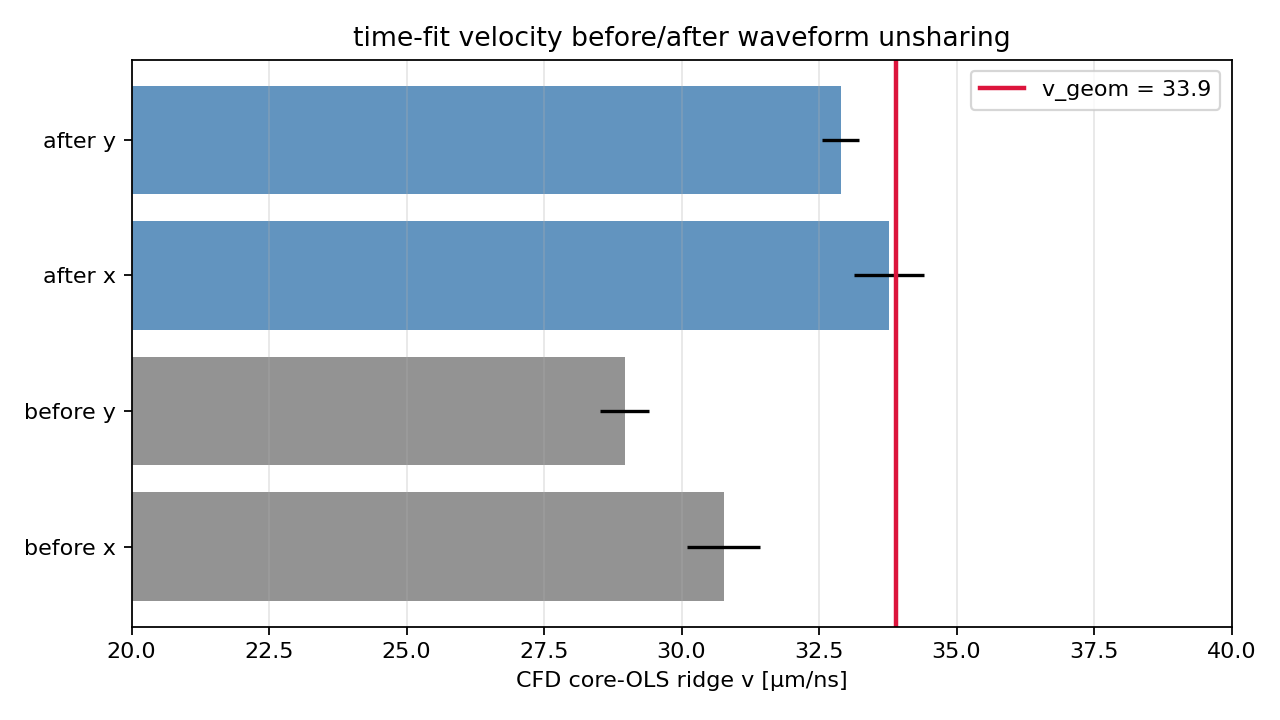
\includegraphics[width=0.62\textwidth]{unsharing_v.png}
\caption{Waveform unsharing prototype.  Top: sharing fractions measured
from vertical tracks per plane (note the larger second-neighbour sharing in
$y$, the resistive-strip direction).  Bottom: time-fit velocity before and
after unsharing --- the corrected values agree with the geometry estimator
(red line).}
\label{fig:unsharing}
\end{figure}

\paragraph{Kernel refinement and the angle payoff.}
A mixed prompt/delayed kernel (fraction $\alpha$ prompt, the rest delayed
by one sample to honour the measured $+\SI{69}{ns}$ neighbour delay;
\texttt{27\_unsharing\_refinement.py}) changes the recovered velocity by
less than $\pm\SI{0.5}{\umns}$ across $\alpha=1\to0$ --- the correction is
robust against the kernel details ($\alpha=0.5$ gives the most consistent
planes, $33.5/33.5$).  The physics payoff is in the \emph{angles}
(Fig.~\ref{fig:unshangles}): with each frame converted at its own ridge
velocity, unsharing \textbf{halves the residual angular bias}
($\pm$\SIrange{4}{4.6}{\degree} $\to$ $\pm$\SIrange{2}{2.6}{\degree}),
\textbf{narrows the small-angle exclusion gap}
($|\thdet|\gtrsim\SIrange{5}{7}{\degree}$ $\to$
$\gtrsim$\SIrange{3}{4}{\degree}), and improves the transition-region
resolution (\SIrange{3}{8}{\degree}: $\sigma_\theta$
\SIrange{2.5}{4.4}{\degree} $\to$ \SIrange{2.1}{2.8}{\degree}), while the
plateau resolution stays at \SIrange{1.5}{2}{\degree}.  The remaining
$\pm\SI{2}{\degree}$ offset is the incompletely-nulled spreading floor
(residual neighbour ratio 0.2--0.34, i.e.\ genuine diffusion charge) and
can be removed as a final additive tan-space calibration.  Per-event fits
lose the skirt strips (clusters shrink toward the direct footprint;
min-strips $4\to3$), trading a few strips per fit for unbiased ones.

\begin{figure}[H]
\centering
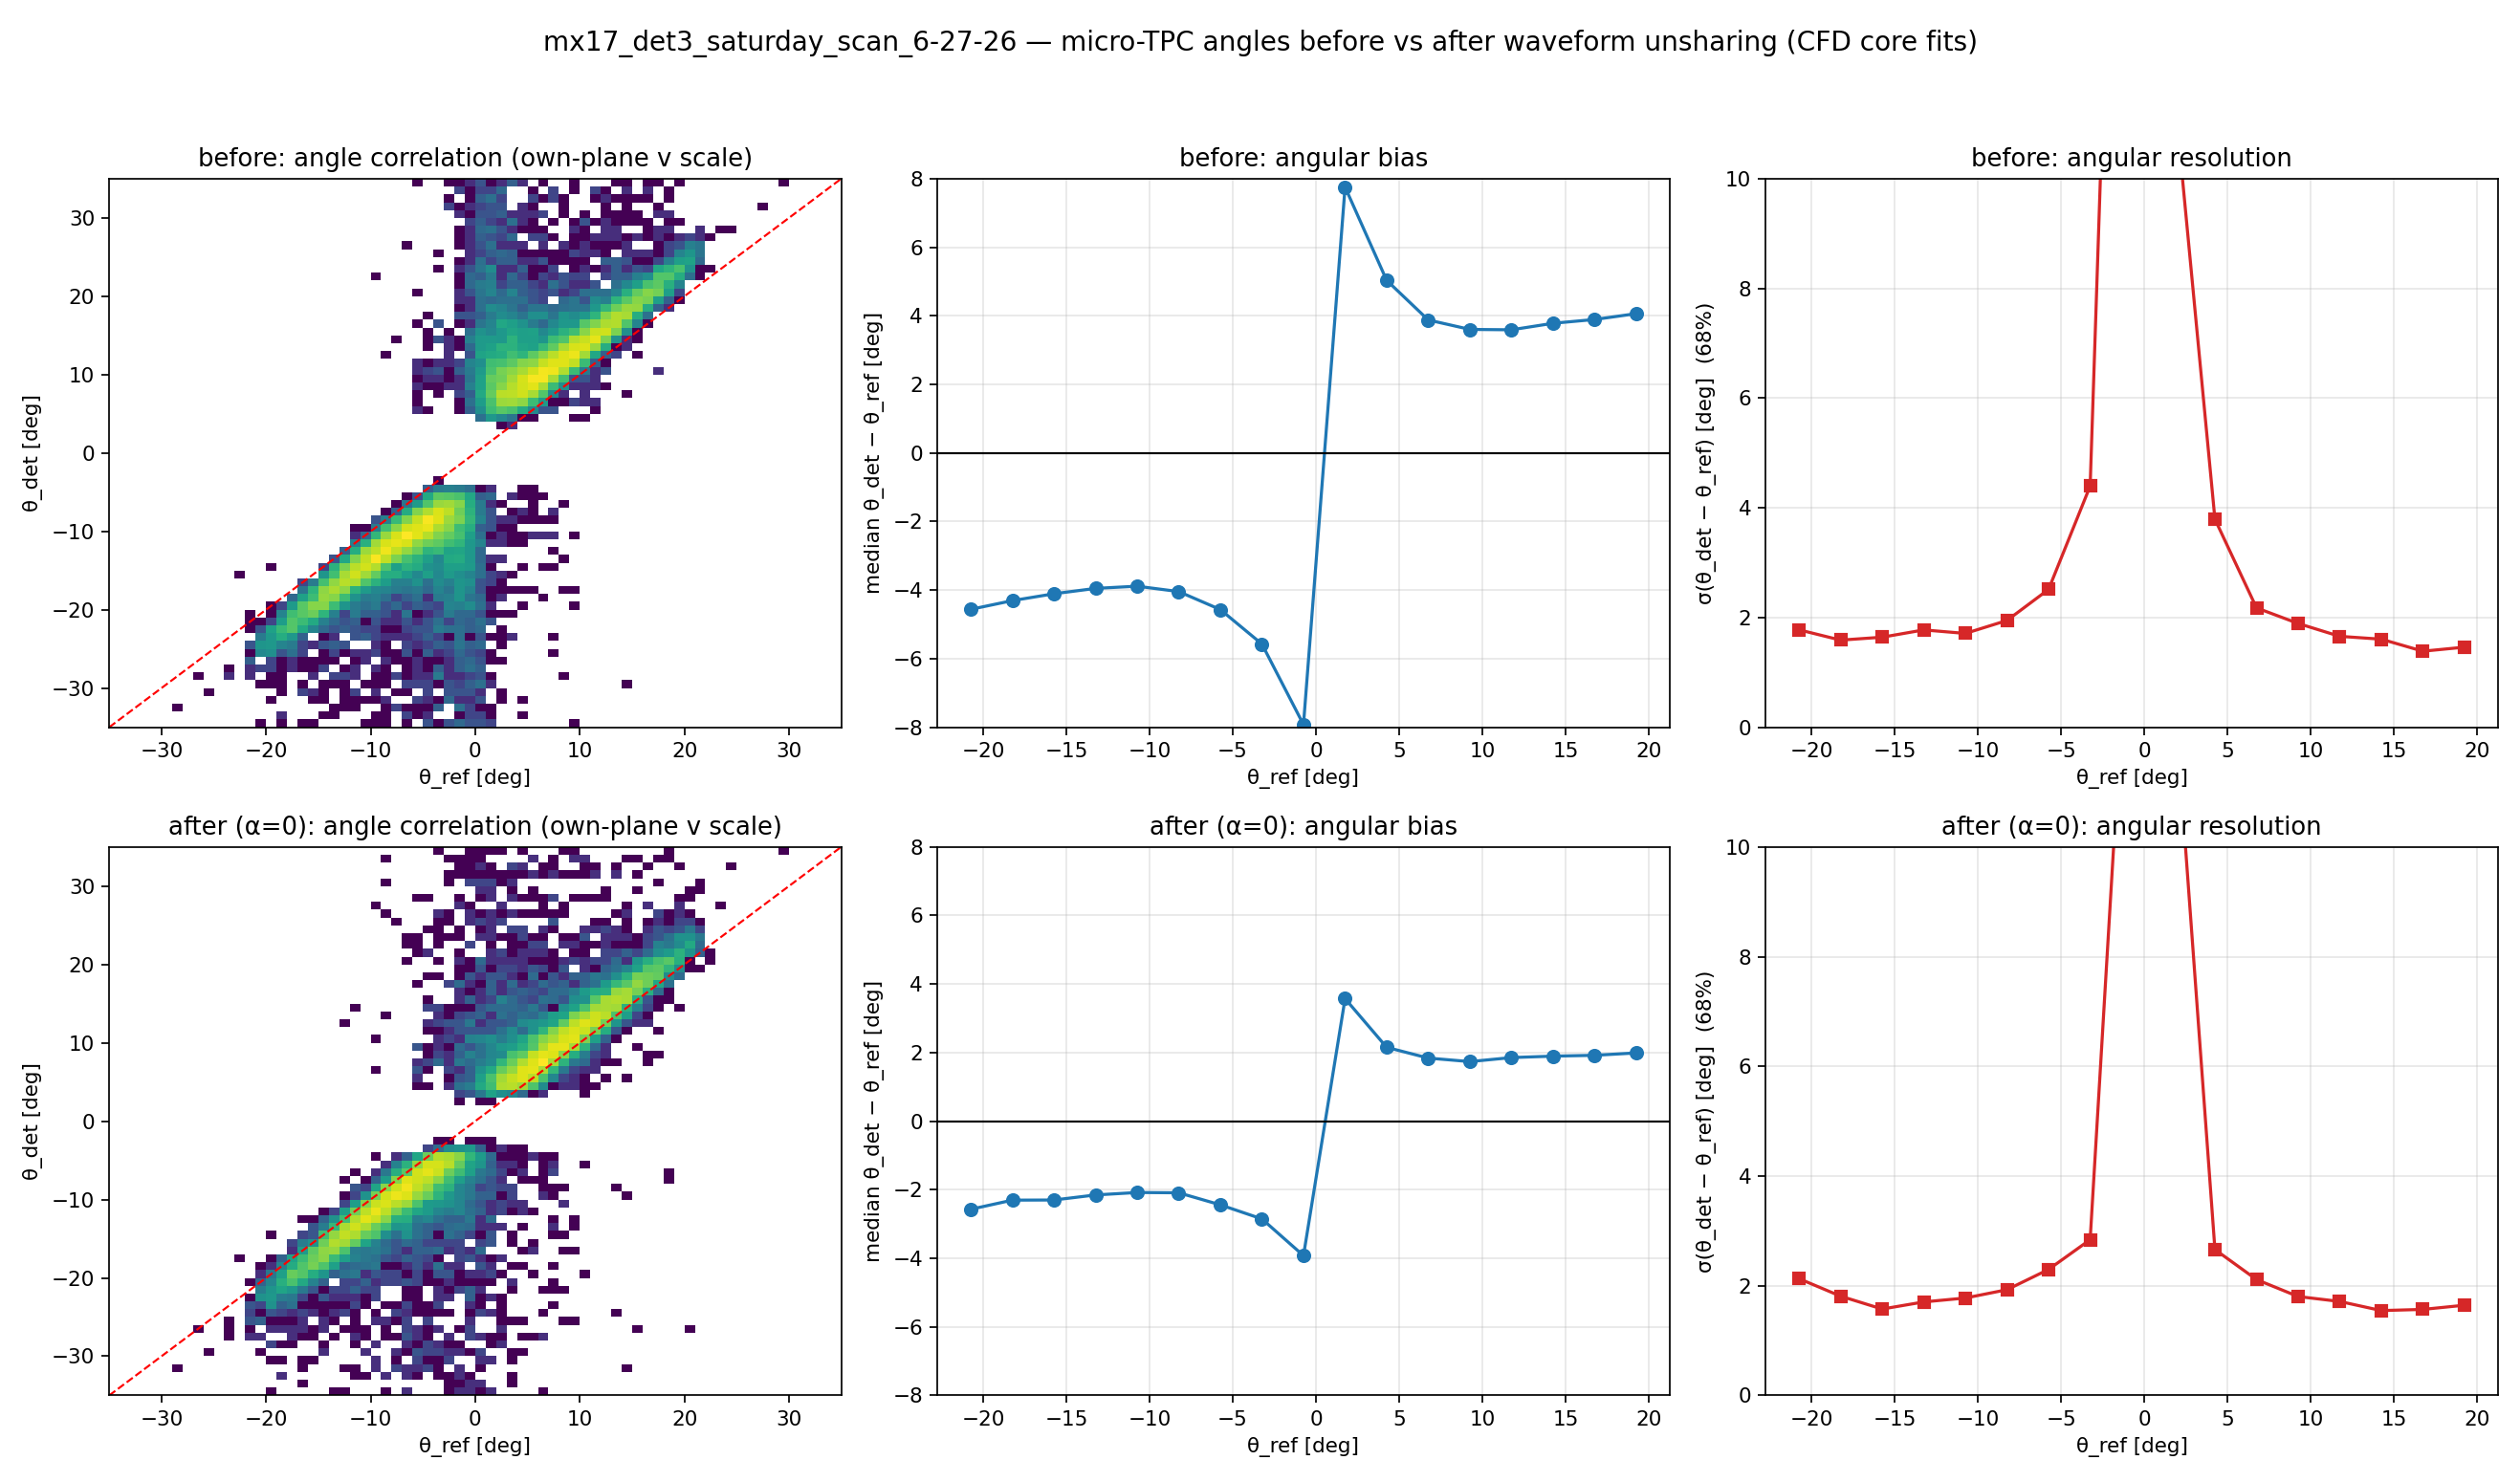
\includegraphics[width=\textwidth]{unsharing_angles.png}
\caption{Micro-TPC angles before (top) and after (bottom) waveform
unsharing, each at its own-plane ridge velocity.  Left: angle correlation
--- the ridge moves onto the diagonal and the small-angle exclusion gap
narrows.  Middle: the sign-following angular bias is halved.  Right:
angular resolution (68\,\% half-width).}
\label{fig:unshangles}
\end{figure}

\paragraph{The last step: one additive constant per plane.}
The $\pm\SI{2}{\degree}$ residual is the same additive, sign-following
structure as the original off-diagonal bias, just 2--3$\times$ smaller ---
it is the spreading floor that unsharing correctly leaves in place
(genuine transverse-diffusion charge, not electronic sharing).  It is
removed by a single calibration constant per plane, measured from the
plateau of the unshared angles themselves
(\texttt{28\_angle\_calibration.py}):
\begin{equation}
  \tan\theta_{\mathrm{corr}} \;=\; \tan\thdet
     \;-\; \mathrm{sign}(\tan\thdet)\cdot b,
  \qquad b_x = 0.033,\; b_y = 0.029 .
\end{equation}
The result (Fig.~\ref{fig:anglecal}) is the final micro-TPC angle
performance achievable on this dataset:
\begin{center}
\textbf{plateau bias $|\Delta\theta| = \SI{0.19}{\degree}$ (median), \quad
plateau resolution $\sigma_\theta = \SI{1.9}{\degree}$ (68\,\%)}
\end{center}
--- from $\pm$\SIrange{4}{5}{\degree} bias in the production analysis to
sub-\SI{0.2}{\degree}, with the correlation ridge sitting on the diagonal.
The plateau resolution itself is now set by diffusion in the (contaminated)
gas, primary-ionisation statistics and the \SI{60}{ns} sampling, not by the
estimator.

\begin{figure}[H]
\centering
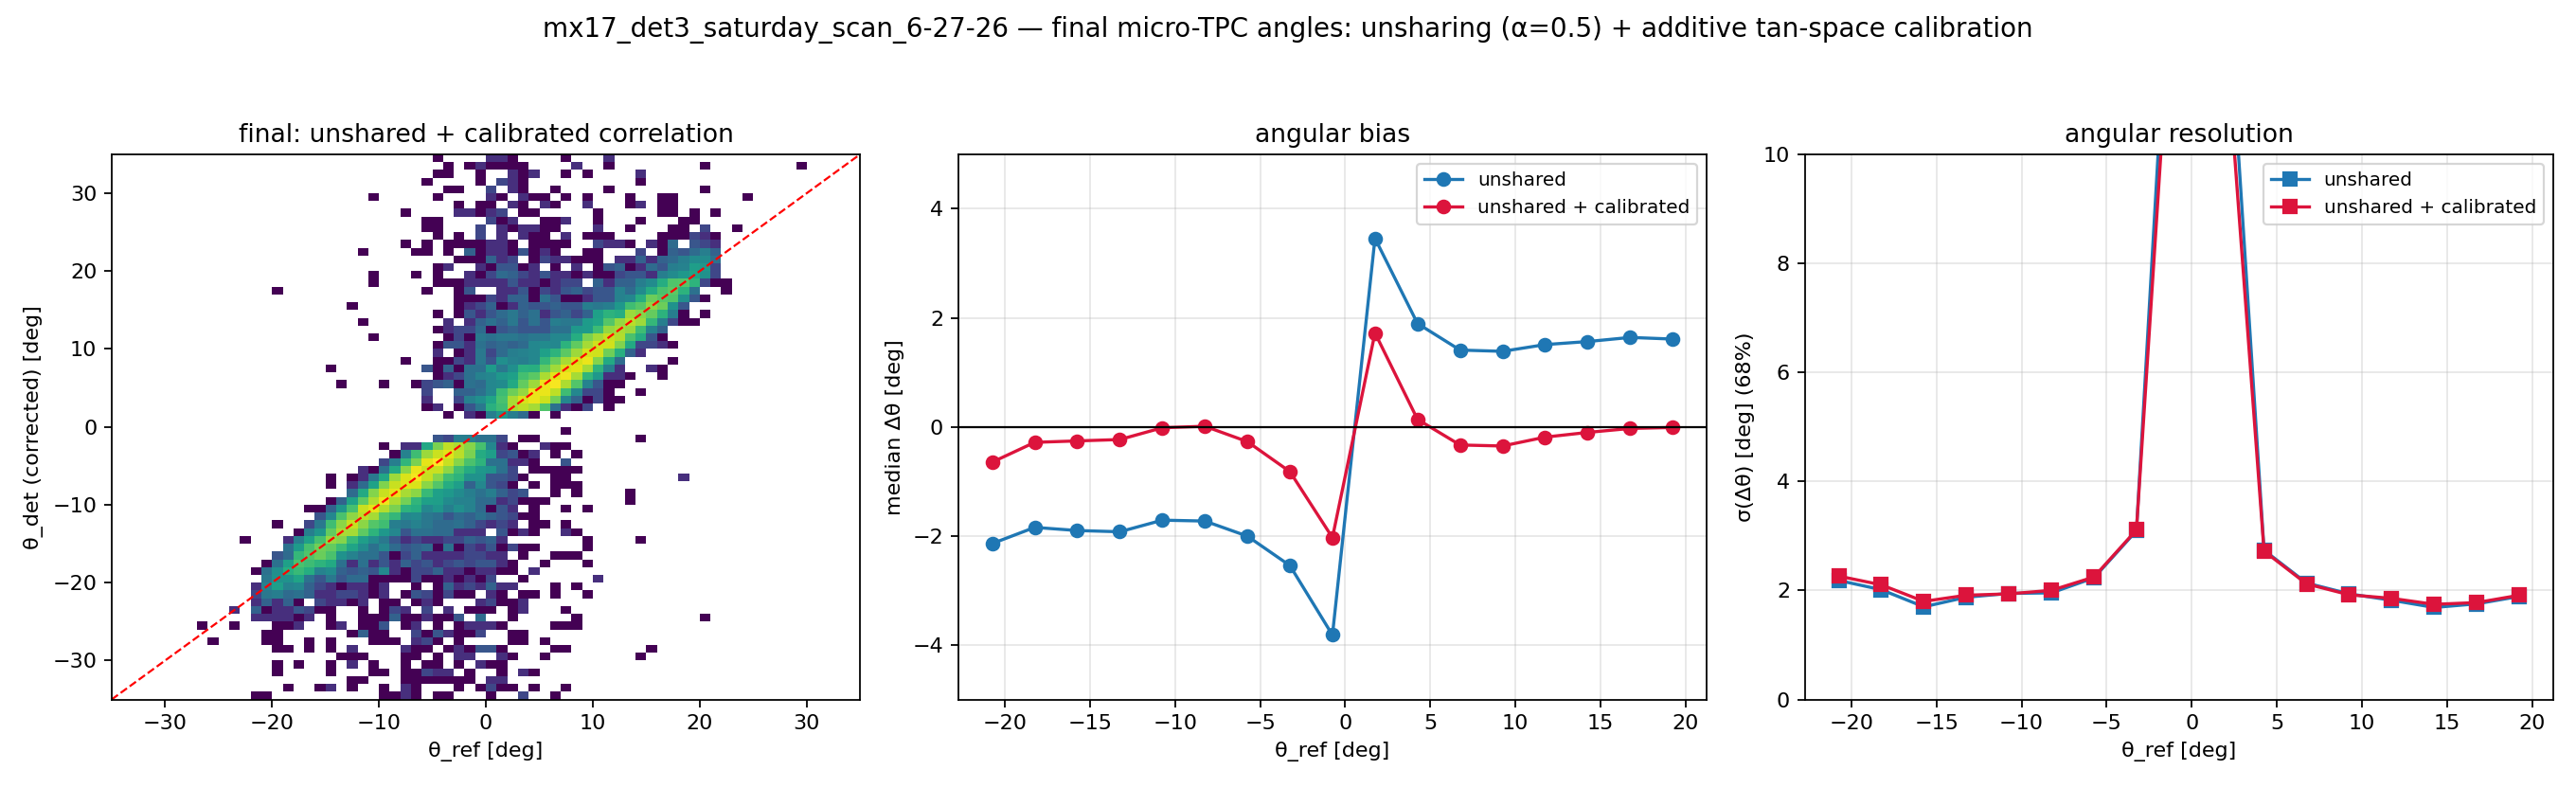
\includegraphics[width=\textwidth]{angle_calibration.png}
\caption{Final micro-TPC angles: unsharing ($\alpha=0.5$ mixed kernel) plus
the additive tan-space calibration.  Left: the corrected correlation sits
on the diagonal.  Middle/right: bias and resolution before and after the
calibration constant --- plateau bias \SI{0.19}{\degree}, resolution
$\approx\SI{1.9}{\degree}$.}
\label{fig:anglecal}
\end{figure}

%=====================================================================
\section{The drift gap: \SI{30}{mm} mechanical, \SI{23}{mm} recorded}
%=====================================================================
\label{sec:gap}

The recorded drift column --- the depth range whose charge produces strips
above threshold --- is measured geometrically by the extent slope of
Sec.~\ref{sec:geomest}: \textbf{\SIrange{21.5}{23.5}{mm}, constant for
$\geq\SI{700}{V}$}, and consistently $\vd^{\mathrm{geom}}\cdot\Tsat \approx
\SI{23}{mm}$.  (The \SI{19.4}{mm} of earlier revisions was this same
quantity evaluated with the biased ridge velocity.)  The mechanical gap is
known to be close to \SI{30}{mm}: the missing \SIrange{6}{8}{mm} at the top
of the gap is charge lost in transit --- captured by electronegative
impurities (attachment) and finished off by the hit threshold --- in the
contaminated gas of Sec.~\ref{sec:gas}.

\subsection{The evidence}

Figure~\ref{fig:gaptest} examines the strip arrival times and amplitudes per
drift-scan point, with times converted to depth via
$z=\vd^{\mathrm{geom}}\,t$:

\begin{itemize}
  \item \textbf{the amplitude decays with depth, identically at every field}
        (Fig.~\ref{fig:ampattach} and top right of Fig.~\ref{fig:gaptest}):
        versus drift \emph{time} the decay timescale changes with HV, but
        versus drift \emph{distance} the \SIrange{700}{1100}{V} curves
        collapse onto one exponential with
        $\lambda \approx \SIrange{16}{18}{mm}$.  Signal loss is a function
        of \emph{how far the charge drifts}, not of time or field --- the
        fingerprint of capture on electronegative impurities (O$_2$), with
        transverse diffusion and charge sharing contributing a milder
        per-strip dilution on top;
  \item \textbf{the arrival-time distribution ends as a threshold crossing,
        not a wall}: flat while the amplitude clears the hit threshold,
        then falling over a few bins around $\Tsat$, with a suppressed tail
        extending beyond.  In depth units the tail endpoints sit at
        \SIrange{28}{34}{mm} (bottom row of Fig.~\ref{fig:gaptest}) ---
        consistent with the \SI{30}{mm} gap, though the far tail mixes
        genuinely deep (attenuated) charge with \emph{late shared/RC}
        signals (Sec.~\ref{sec:timing}), so it is a consistency check
        rather than a precision gap measurement;
  \item \textbf{no observable requires a short gap}: the single-strip pulse
        widths and the time spans all reflect the \emph{recorded} column,
        and the recorded column is set by gas quality, not electrode
        spacing.
\end{itemize}

\begin{figure}[H]
\centering
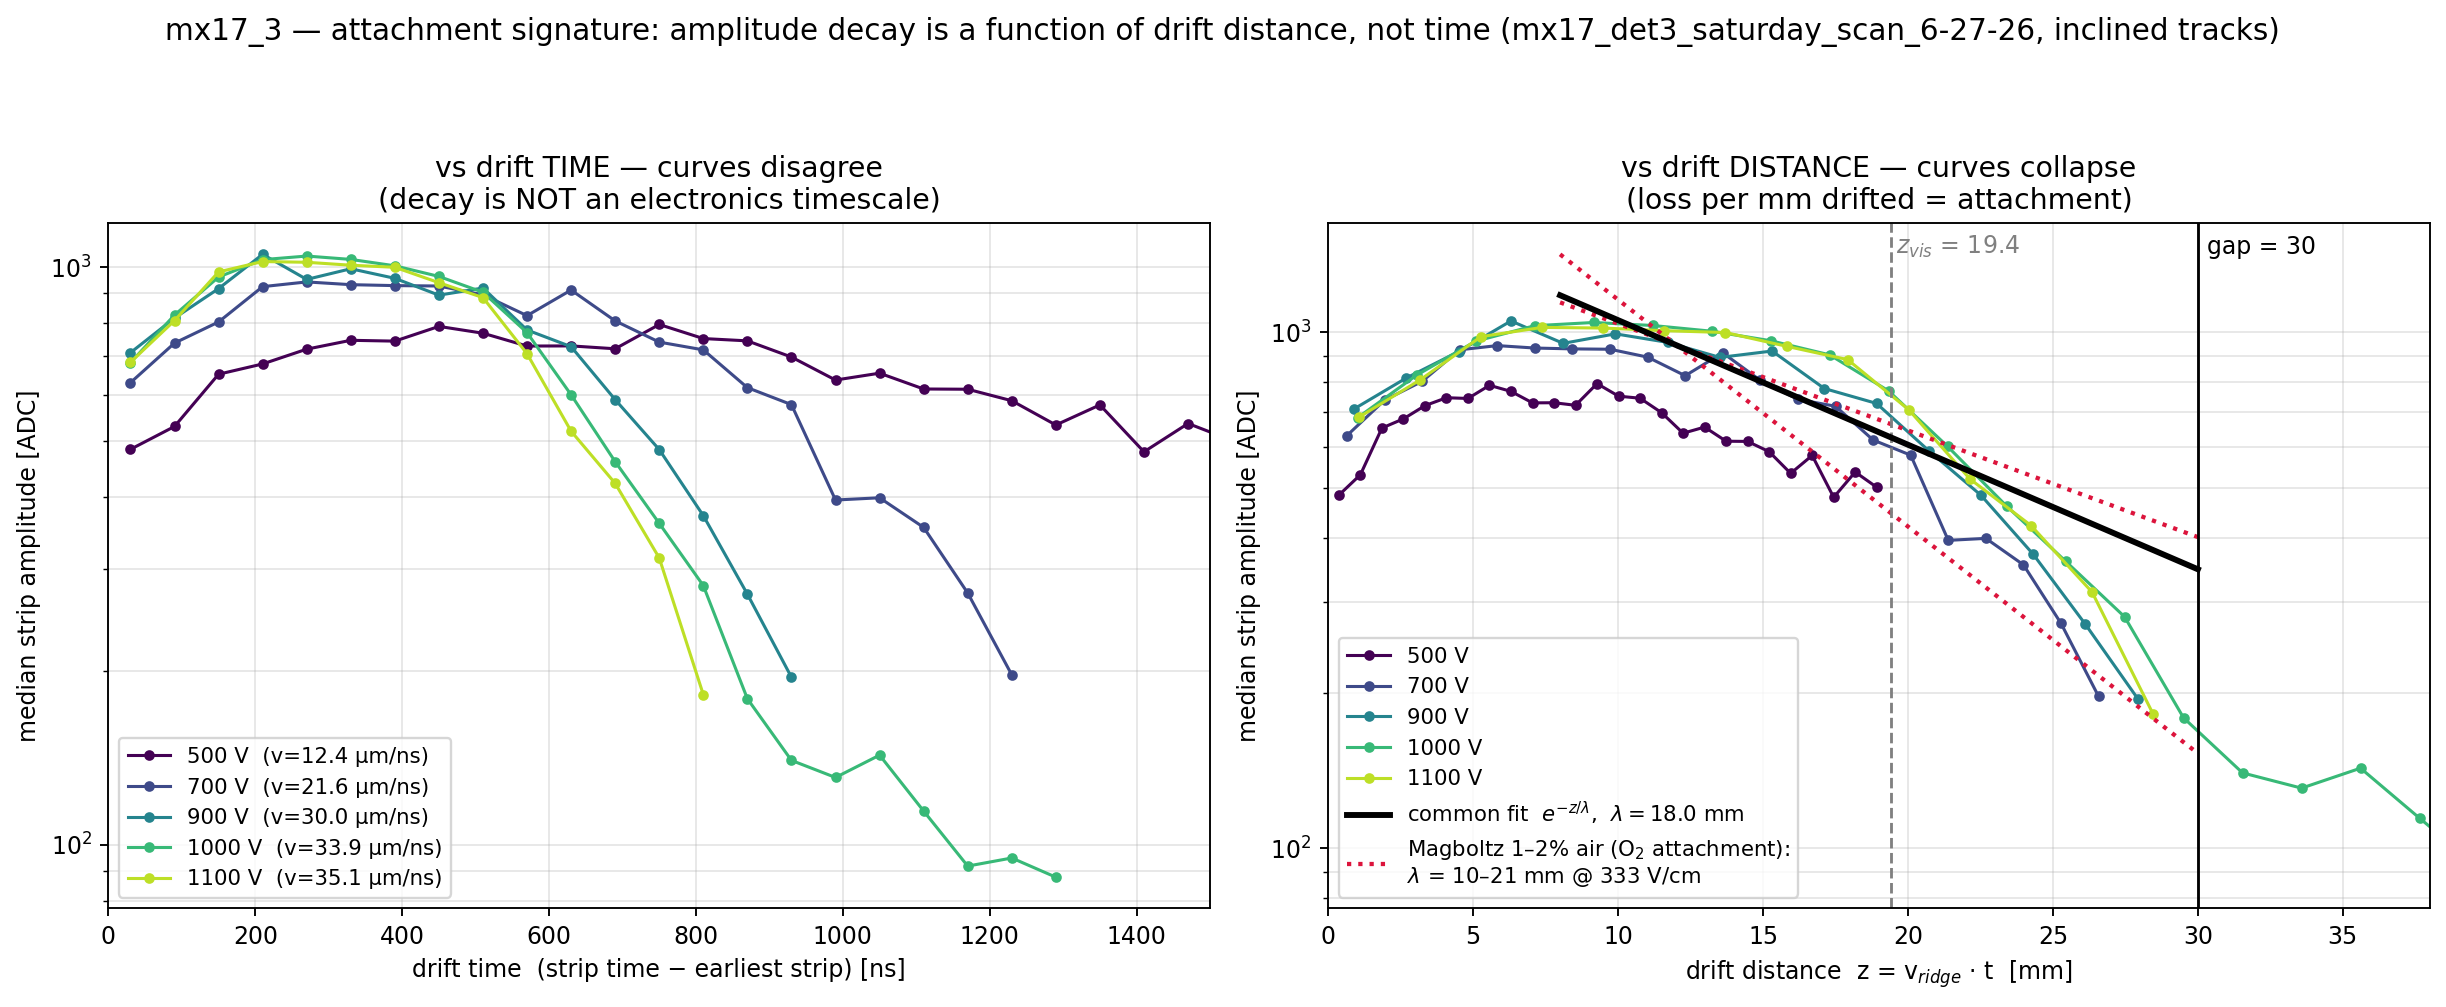
\includegraphics[width=\textwidth]{amplitude_attachment.png}
\caption{The attachment signature in one plot
(\texttt{19\_amplitude\_attachment\_plot.py}).  Median strip amplitude for
inclined tracks, per drift HV.  Left: versus drift \emph{time} --- the decay
timescale changes with drift field (\SI{1100}{V} dies by \SI{800}{ns} while
\SI{500}{V} is still flat at \SI{1400}{ns}), so it is not an electronics
timescale (ion tail, shaping, undershoot would be identical curves).  Right:
the same data versus drift \emph{distance} $z=\vd^{\mathrm{geom}} t$ --- the
\SIrange{700}{1100}{V} curves collapse onto a single exponential,
$\lambda \approx \SI{18}{mm}$ over \SIrange{8}{24}{mm}, inside the Magboltz
O$_2$-attachment band for $\sim$\SI{1}{\percent} air (red dotted).  Loss per
millimetre drifted is electron capture.}
\label{fig:ampattach}
\end{figure}

\begin{figure}[H]
\centering
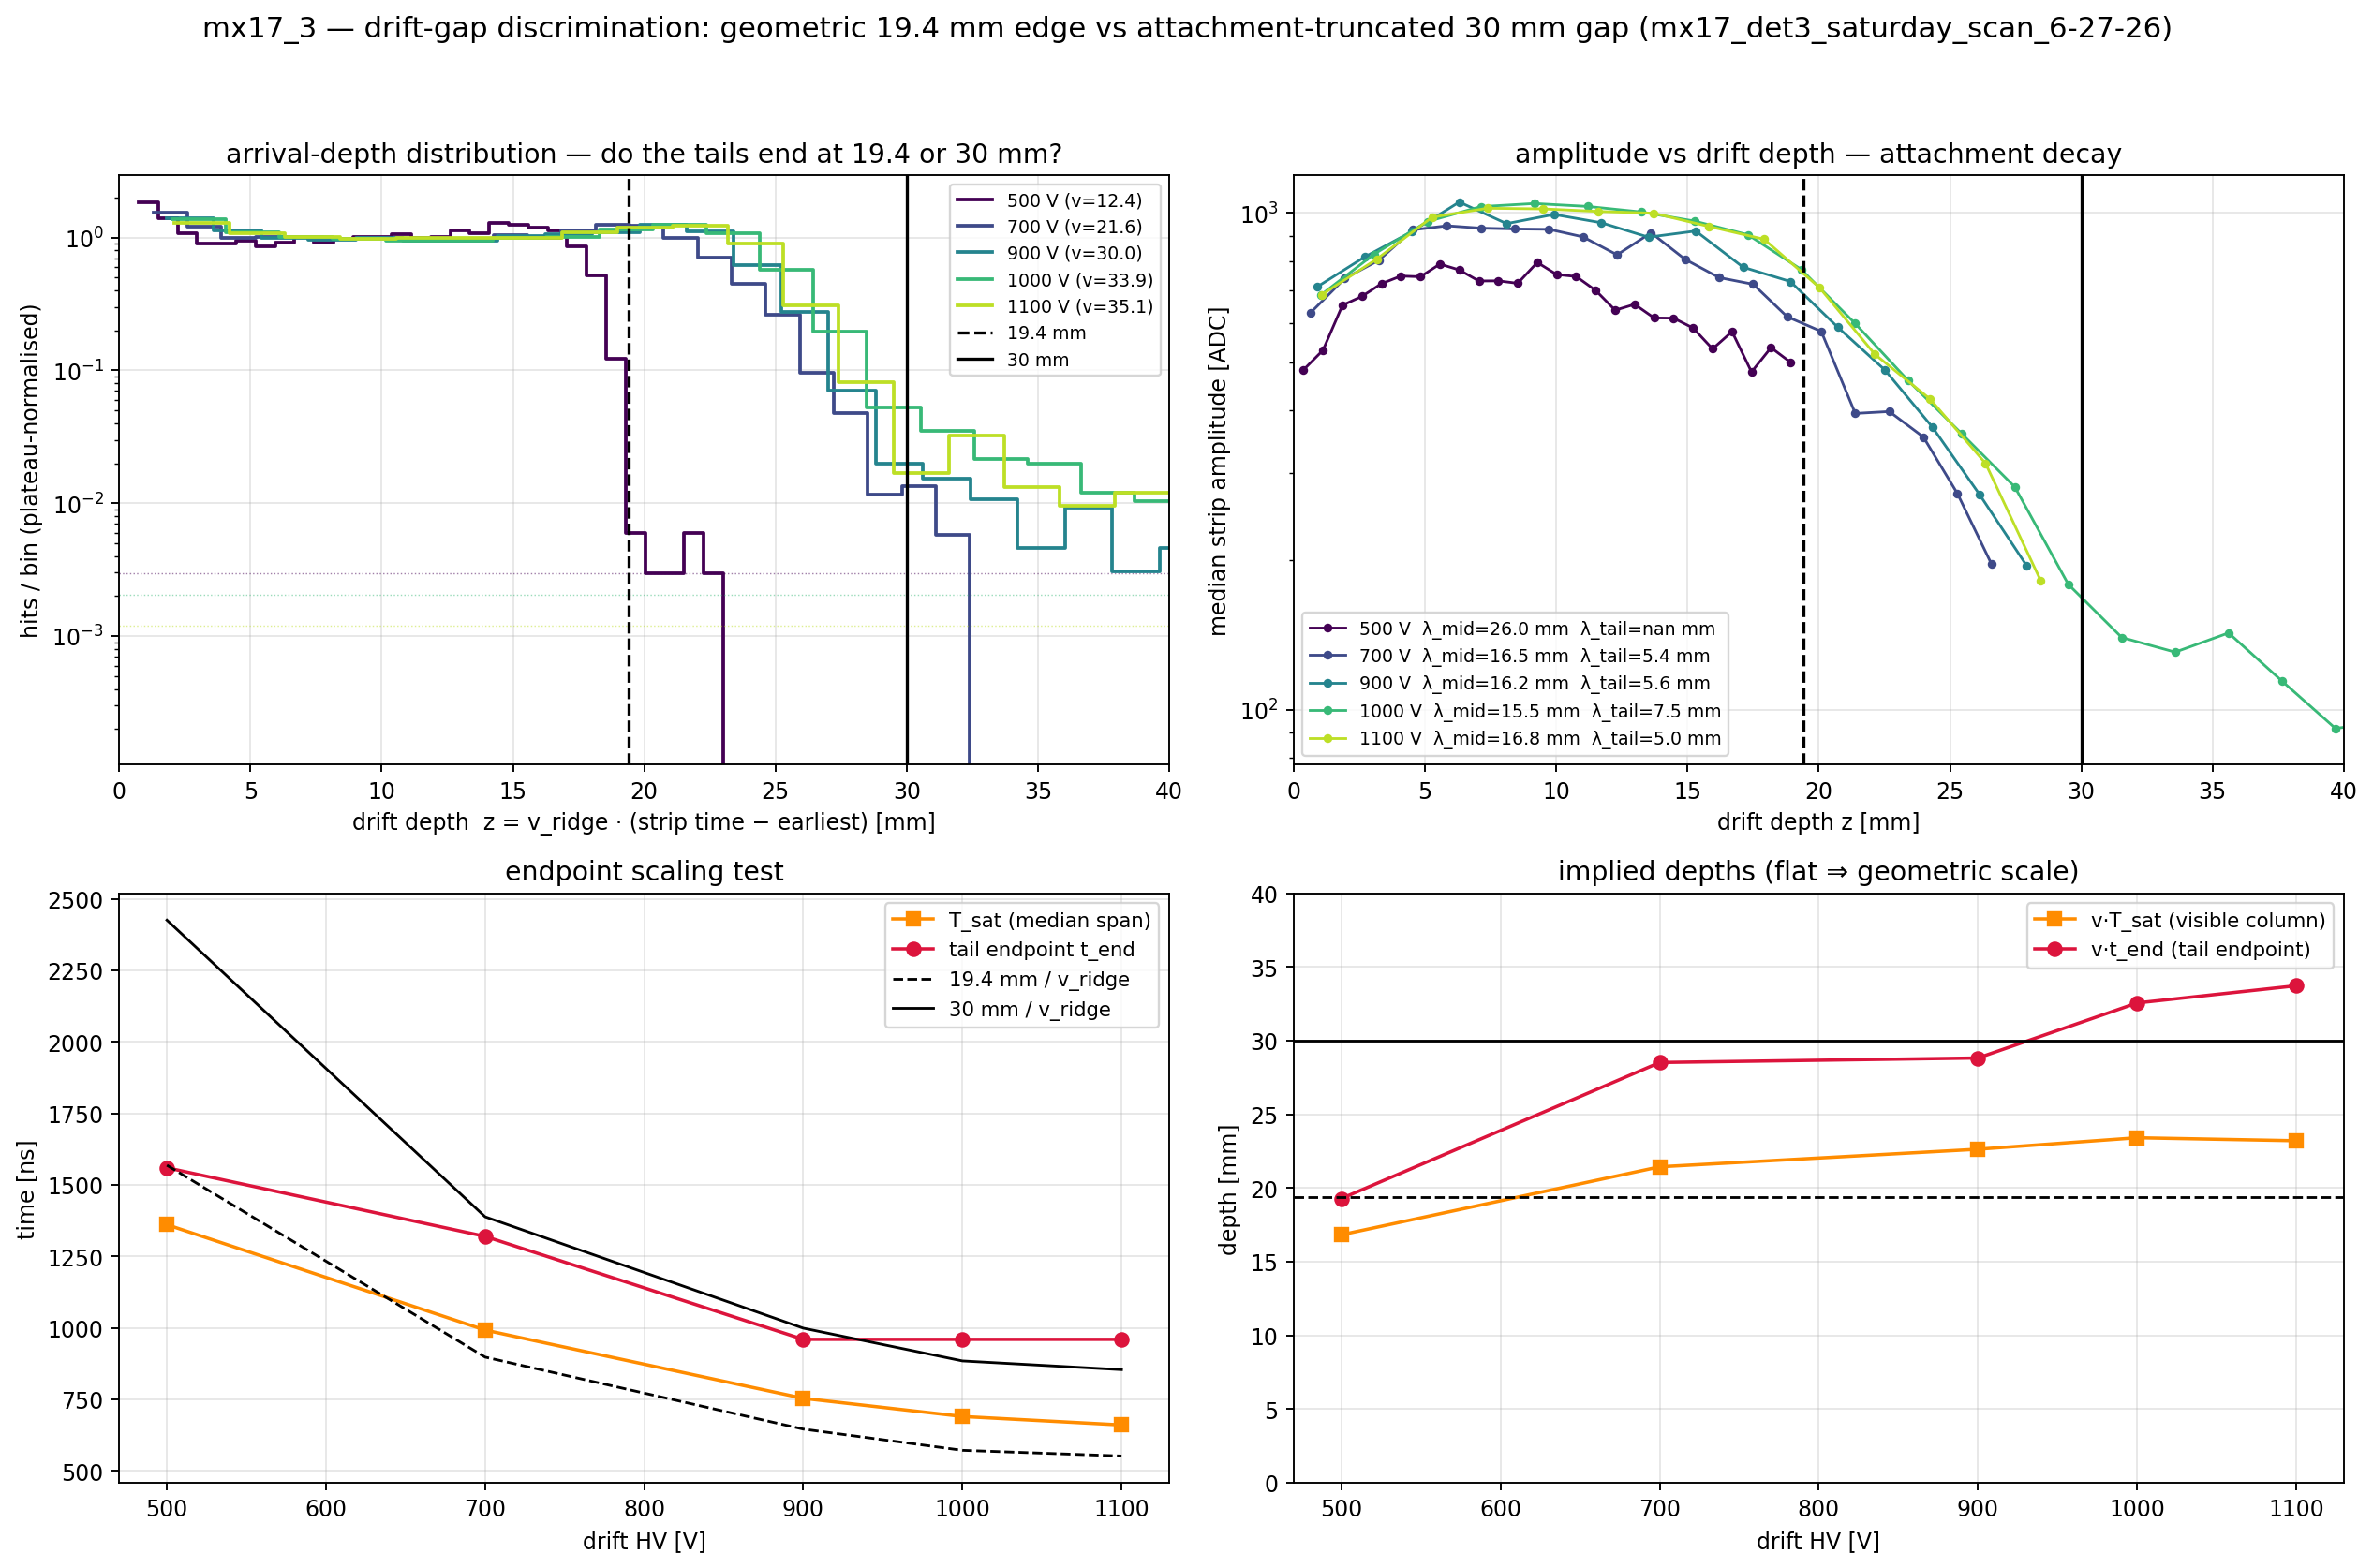
\includegraphics[width=\textwidth]{gap_attachment_test.png}
\caption{Arrival-time structure per drift HV
(\texttt{17\_gap\_attachment\_test.py}, depth scale
$z=\vd^{\mathrm{geom}}t$).  Top left: strip arrival-depth distributions
(plateau-normalised, log scale) --- flat plateau over the recorded column,
threshold roll-off, suppressed tail.  Top right: median strip amplitude vs
depth --- one universal decay curve for all fields.  Bottom: the time-span
plateau $\Tsat$ and the tail endpoint versus HV, in time (left) and depth
(right); the recorded column (orange) is constant at
\SIrange{21.5}{23.5}{mm} and the tail endpoints (red) straddle the
\SI{30}{mm} gap.}
\label{fig:gaptest}
\end{figure}

\begin{figure}[H]
\centering
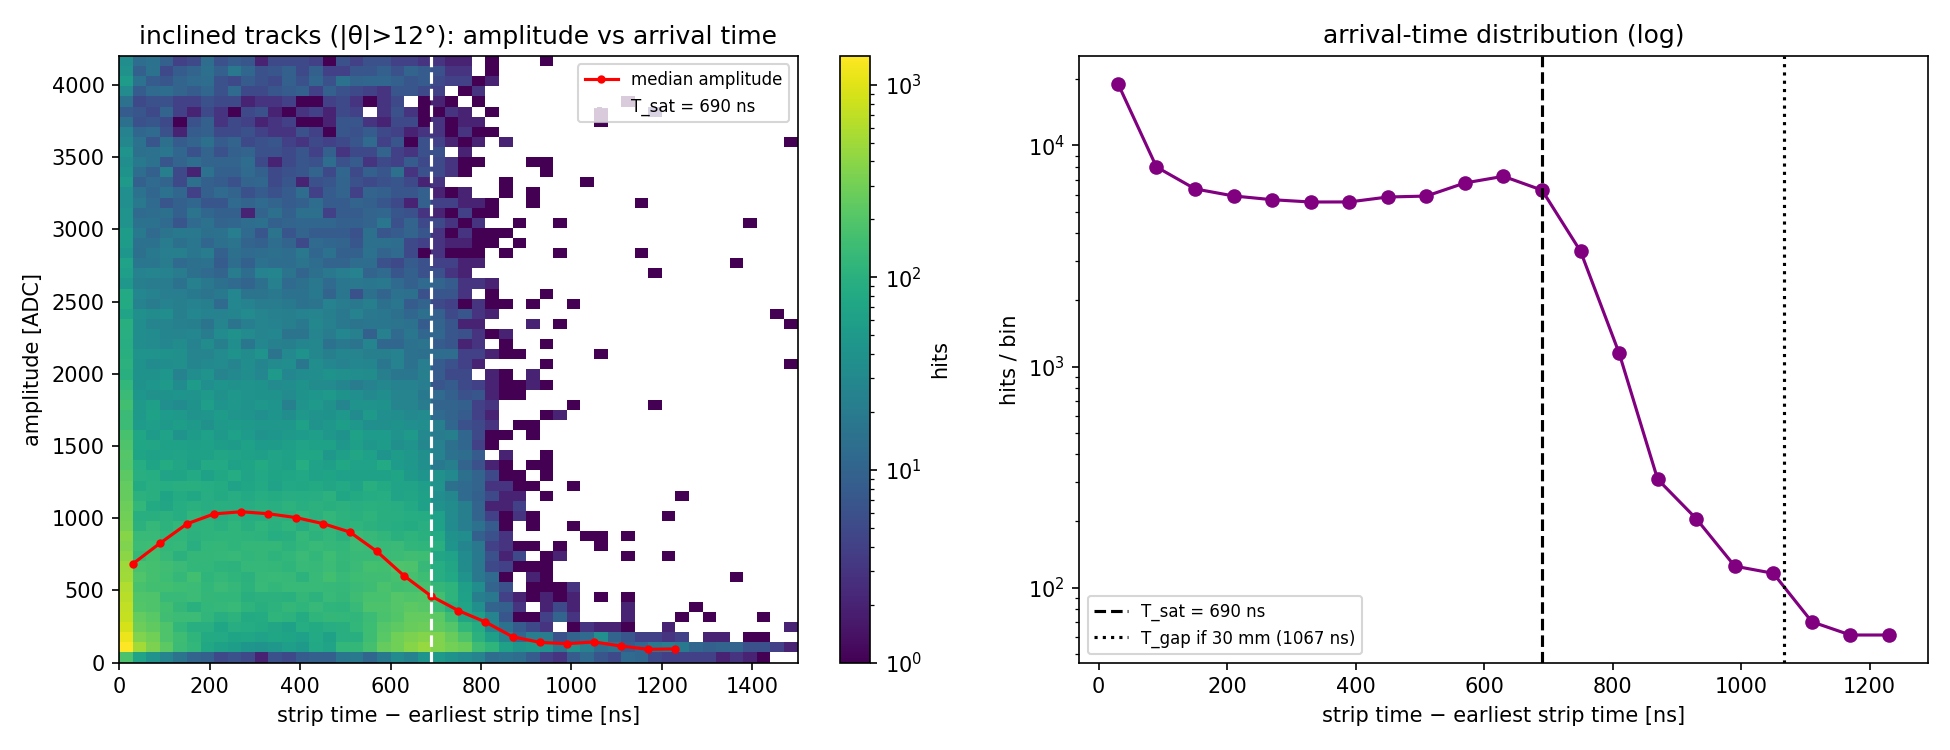
\includegraphics[width=0.94\textwidth]{amplitude_vs_drifttime.png}
\caption{Inclined tracks, 2.4\,h run. Left: strip amplitude vs arrival time;
the median (red) decays steadily with drift time.  Right: the arrival-time
distribution --- flat to $\Tsat=\SI{690}{ns}$ (dashed), then an exponential
fall into the noise floor; the tail beyond $\Tsat$ mixes attenuated deep
charge with late shared/RC signals.}
\label{fig:ampvstime}
\end{figure}

\subsection{Consistency of the other observables}

The single-strip pulse widths (Fig.~\ref{fig:pulsewidth}) measure the
duration over which a vertical track's lead strip stays above threshold ---
i.e.\ the \emph{recorded} column's drift time.  Their $\sim\SI{700}{ns}$
scale is consistent with the picture and carries no independent information
about the mechanical gap.

\begin{figure}[H]
\centering
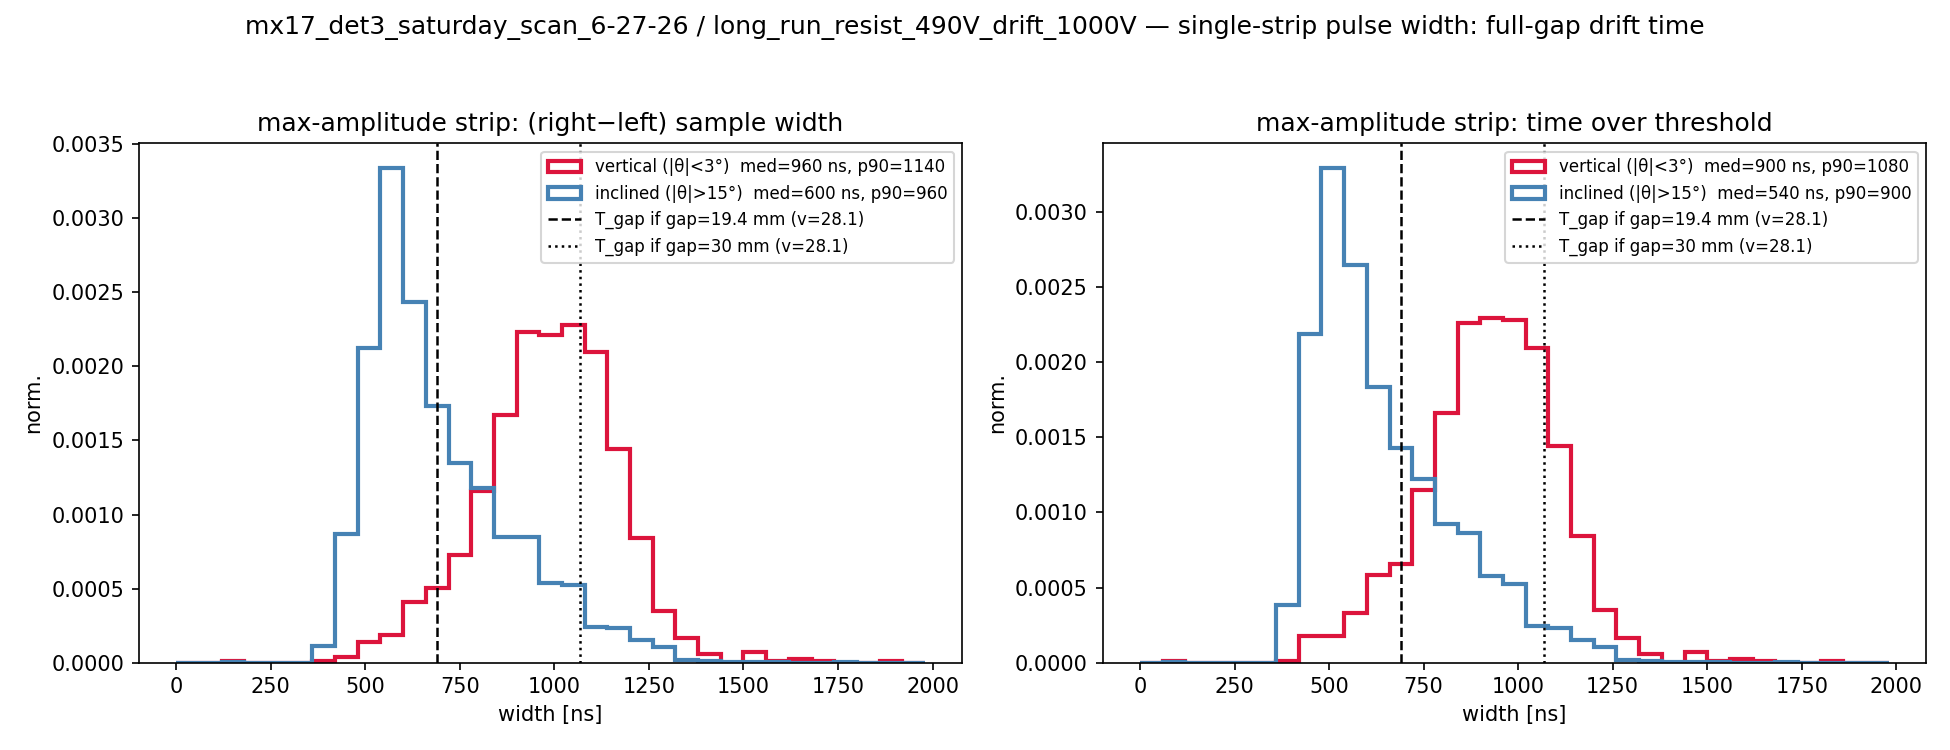
\includegraphics[width=0.94\textwidth]{pulse_width_gap.png}
\caption{Single-strip pulse width for vertical ($|\theta|<\SI{3}{\degree}$,
red) versus inclined ($|\theta|>\SI{15}{\degree}$, blue) tracks; the
vertical-track widths reflect the drift time of the \emph{recorded} column
($\approx\SI{700}{ns}$ at \SI{1000}{V}).}
\label{fig:pulsewidth}
\end{figure}

\subsection{Interpretation and consequences}

\begin{itemize}
  \item \textbf{Field scale}: with $g=\SI{30}{mm}$ the drift field is
        $E = V_{\mathrm{drift}}/\SI{3.0}{cm}$ (\SI{1000}{V} $\to$
        \SI{333}{\volt\per\centi\meter}); Sec.~\ref{sec:gas} uses this
        throughout.
  \item \textbf{$z_{\mathrm{rec}}$ is a gas-quality number, not a detector
        constant}: it is where the survival probability
        $\exp(-z/\lambda_{\mathrm{att}})$ meets the threshold.  Cleaning the
        gas should push the recorded column towards the full \SI{30}{mm} ---
        lengthening $\Tsat$ (mind the \SI{1.92}{\micro s} window:
        \SI{30}{mm} at \SI{34}{\umns} is \SI{880}{ns}, comfortable),
        increasing the collected charge, and shrinking the off-diagonal
        offset of Sec.~\ref{sec:offdiag}.
  \item \textbf{Charge budget}: roughly a quarter of each track's ionisation
        is currently lost in transit, and what survives from mid-column is
        attenuated --- a direct efficiency and signal-to-noise cost on top of
        the drift-speed problem.
  \item The \SI{60}{ns} DREAM sampling period assumption still deserves a
        one-line confirmation; it rescales $\vd$ and all times together but
        no conclusion here depends on it.
\end{itemize}

%=====================================================================
\section{Gas diagnosis: air/moisture contamination of the Ar/iso 95/5}
%=====================================================================
\label{sec:gas}

\subsection{The discrepancy}

With the \SI{30}{mm} field scale
($E = V_{\mathrm{drift}}/\SI{3.0}{cm}$; \SI{1000}{V} $\to$
\SI{333}{\volt\per\centi\meter}) the geometry-based $\vd(E)$ can be
confronted with Magboltz (Garfield++ \texttt{MediumMagboltz}, Saclay
pressure \SI{745.8}{Torr}, \SI{293}{K}).  For \emph{clean}
Ar/iC$_4$H$_{10}$ 95/5 the prediction peaks at \SI{41}{\umns} near
\SI{210}{\volt\per\centi\meter} and \emph{decreases} slowly above; the
measurement instead rises monotonically over the whole scan, is a factor
$\sim$3 low at \SI{167}{\volt\per\centi\meter} (\SI{12.4} vs
$\sim$\SI{40}{\umns}), and reaches only \SI{33.9}{\umns} at the operating
field where clean gas predicts \SI{39}{\umns}.  The shape disagreement is
the crucial part: no rescaling of times, fields or gap can turn a curve
that peaks at \SI{210}{\volt\per\centi\meter} into one still rising at
\SI{370}{\volt\per\centi\meter}.  This is a \emph{gas property} --- and it
is robust against the velocity-estimator question: at \SI{700}{V} the raw
time span alone bounds $\vd(\SI{233}{V/cm}) \leq \SI{30}{mm}/\SI{992}{ns}
= \SI{30.2}{\umns}$, far below the clean-gas \SI{41}{\umns}.

\subsection{Candidate mixtures}

{\sloppy Magboltz was run for candidate gases over the drift-field range
(\texttt{mm\_drift\_velocity\_candidates.py},
\texttt{mm\_attachment\_\{table,air\_candidates\}.py} locally, and the fine
water grid \texttt{mm\_water\_grid\_lxplus.py} on lxplus);
Fig.~\ref{fig:vgeomscan} and Table~\ref{tab:candidates}:\par}

\begin{table}[H]
\centering\small
\begin{tabular}{l S[table-format=2.2] l}
\toprule
hypothesis & {RMS dev.\ [\si{\umns}]} & verdict \\
\midrule
Ar/iso 95/5 + \SI{1}{\percent} H$_2$O + \SI{1}{\percent} N$_2$
    & 0.84 & \textbf{best fit} \\
Ar/iso 95/5 + \SI{1}{\percent} H$_2$O    & 1.12 & \textbf{consistent} \\
Ar/iso 95/5 + \SI{1}{\percent} H$_2$O + \SI{2}{\percent} air & 1.35 & consistent \\
Ar/iso 95/5 + \SI{1.2}{\percent} H$_2$O  & 2.80 & slightly too slow \\
Ar/iso 95/5 + \SI{0.8}{\percent} H$_2$O  & 4.66 & too fast \\
Ar/CO$_2$ 90/10 (wrong bottle)           & 5.41 & excluded (also by gain \& attachment) \\
Ar/iso 95/5 + \SIrange{1.5}{3}{\percent} H$_2$O & {7--19} & excluded \\
Ar/iso 95/5 + dry air only               & {14--16} & no $\vd$ suppression \\
Ar/iso 95/5 (nominal, clean)             & 16.1 & excluded \\
Ar/iso 90/10 \ldots\ 80/20               & {9--17} & iso-rich stays fast: excluded \\
\bottomrule
\end{tabular}
\caption{RMS deviation between each Magboltz candidate and the
geometry-based $\vd(E)$ (\SIrange{500}{1100}{V} points, $E=V/\SI{3.0}{cm}$).
The water fraction is bracketed tightly: \SIrange{1.0}{1.1}{\percent} H$_2$O,
with N$_2$/air co-contamination preferred.  (Earlier revisions, using the
biased ridge velocities, had favoured \SIrange{2}{2.5}{\percent} and then
Ar/CO$_2$ --- the estimator fix collapses the ambiguity.)}
\label{tab:candidates}
\end{table}

Two other observables corroborate and close the identification:

\paragraph{Amplification.}  A Magboltz Townsend-coefficient comparison over
the \SI{150}{\micro\meter} amplification gap
(\texttt{mm\_townsend\_compare.py}) puts every iso-gain point of
Ar/CO$_2$ 90/10 about \SI{50}{V} \emph{above} Ar/iso 95/5 (gain $10^2$:
\SI{528}{V} vs \SI{475}{V}; gain $10^3$: \SI{631}{V} vs \SI{587}{V}).  The
observed turn-on at \SI{425}{V} with full plateau by \SI{455}{V}
(Sec.~\ref{sec:hvscans}) matches the Ar/iso expectation; with Ar/CO$_2$ the
whole efficiency curve would sit $\sim$\SI{50}{V} higher.  Percent-level
H$_2$O/air, by contrast, leaves the gain curve essentially untouched.

\paragraph{Attachment.}  Clean Ar/CO$_2$ does not attach electrons at drift
fields ($\eta = 0$ in Magboltz) --- it cannot produce the amplitude decay of
Fig.~\ref{fig:gaptest}.  Neither, notably, can water alone: Magboltz gives
$\eta = 0$ for all Ar/iso + H$_2$O mixtures at these fields (water's
dissociative-attachment threshold, $\sim$\SI{5}{eV}, is far above drift
energies).  The measured decay needs \textbf{oxygen}.

\subsection{The attachment cross-check closes on O$_2$}

Figure~\ref{fig:attclose} compares the measured amplitude-decay length from
the drift scan with the Magboltz attachment length $1/\eta(E)$ for
air-doped mixtures.  On the corrected depth scale the measured mid-column
$\lambda \approx \SIrange{16}{18}{mm}$ at
\SIrange{230}{370}{\volt\per\centi\meter} matches the \SI{1}{\percent}-air
prediction (\SI{0.21}{\percent} O$_2$,
$\lambda\approx\SIrange{16}{21}{mm}$):
\textbf{an O$_2$ fraction of $\sim$\SIrange{0.15}{0.25}{\percent}
reproduces the observed signal loss} --- the same $\sim$\SI{1}{\percent}
air-equivalent that the velocity fit prefers as N$_2$ co-contamination.
(Water \emph{enhances} the three-body O$_2$ attachment: with
\SI{1}{\percent} H$_2$O present, Magboltz gives $\lambda=\SI{4.9}{mm}$
already at \SI{0.42}{\percent} O$_2$, so the true O$_2$ fraction sits at
the low end.  The measured $\lambda$ also absorbs some per-strip dilution
from diffusion and sharing.)

\begin{figure}[H]
\centering
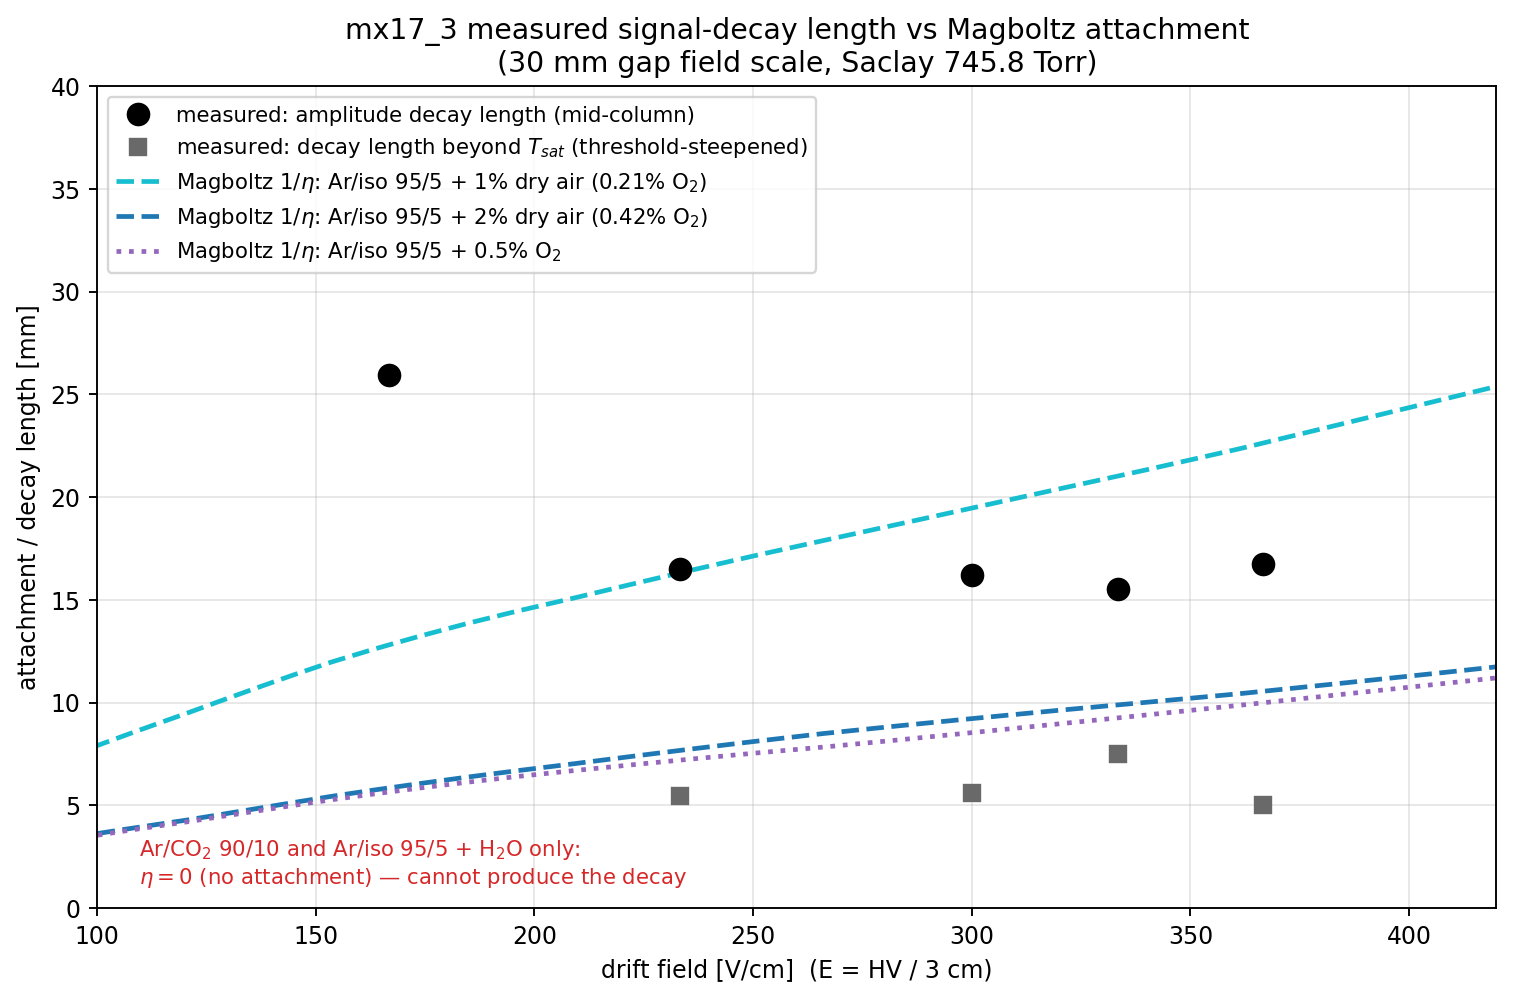
\includegraphics[width=0.85\textwidth]{attachment_vs_magboltz.png}
\caption{Measured signal-decay length vs drift field (black: mid-column;
grey: beyond $\Tsat$, steepened by the threshold), compared with Magboltz
attachment lengths $1/\eta$ for O$_2$-doped Ar/iso 95/5.  Mixtures without
O$_2$ (clean Ar/CO$_2$, Ar/iso + H$_2$O only) predict no attachment at all.}
\label{fig:attclose}
\end{figure}

\subsection{Interpretation: one contamination, both anomalies}

Everything points at a single cause --- \textbf{air and moisture in the
drift gas} at the percent level:
\begin{itemize}
  \item \SIrange{1.0}{1.1}{\percent} H$_2$O reproduces the slow,
        monotonically rising $\vd(E)$ point-by-point (RMS
        \SI{0.84}{\umns} with N$_2$; water's huge dipole cross-section
        thermalises the electrons at low field).  That is
        $\sim$\SIrange{40}{50}{\percent} relative humidity worth of water
        --- ordinary damp-air/outgassing levels, not a flooded line;
  \item $\sim$\SIrange{0.15}{0.25}{\percent} O$_2$ ($\sim$\SI{1}{\percent}
        air-equivalent, matching the preferred N$_2$ co-contamination)
        reproduces the attachment that truncates the recorded drift column
        at $\approx\SI{23}{mm}$ (Sec.~\ref{sec:gap});
  \item the amplification is insensitive to impurities at this level ---
        consistent with the resist-HV scans matching clean-gas gain;
  \item water in excess of the air-implied share is expected: H$_2$O
        permeates plastics and outgasses from glued structures far faster
        than O$_2$ enters, the classic signature of an unflushed or
        under-flushed detector volume.
\end{itemize}

Likely entry points: an unflushed detector volume, permeable or long
tubing, very low flow rate, or a leaky fitting.  \textbf{The June campaign
is closed and cannot be re-run}, so a fresh-gas re-scan is not available as
a check; the identification instead rests on the internal closure achieved
here --- velocity shape (\SI{0.84}{\umns} RMS over five field points),
attachment length, gain behaviour, and the exclusion of every tested
alternative --- and can be tightened further with existing data only:
\begin{itemize}
  \item apply the same chain (geometry estimator + amplitude-vs-depth) to
        the \emph{other} detectors' June runs: they shared the gas line, so
        the same $\vd(E)$ and $\lambda_{\mathrm{att}}$ are predicted ---
        a genuine out-of-sample test (decoded waveforms for those runs
        remain on the lxplus archive);
  \item the drift-scan points themselves already provide five independent
        fields; any future gas hypothesis must thread all of them
        simultaneously, which is a strong constraint.
\end{itemize}

Beyond drift speed, the contamination costs signal: roughly a quarter of
each track's charge is captured before reaching the mesh, and the enhanced
diffusion feeds the charge-spreading width $w$ of Sec.~\ref{sec:offdiag}.
Cleaning the gas should improve efficiency, signal-to-noise, micro-TPC angle
quality, and the small-angle exclusion gap simultaneously.

%=====================================================================
\section{Resist-HV scans}
%=====================================================================
\label{sec:hvscans}

Two resist scans bracket the operating point at drift \SI{1000}{V}
(Fig.~\ref{fig:hvscans}): a wide scan (\SIrange{425}{525}{V}, 11 points) and
a fine repeat (\SIrange{460}{520}{V}).  Both use the long-run alignment with
a translation refit per point; efficiency is counted in a fixed active box
with the standard $R=\SI{5}{mm}$ matching, and the spark fraction (events
with $>50$ strips firing) is overlaid.

\begin{figure}[H]
\centering
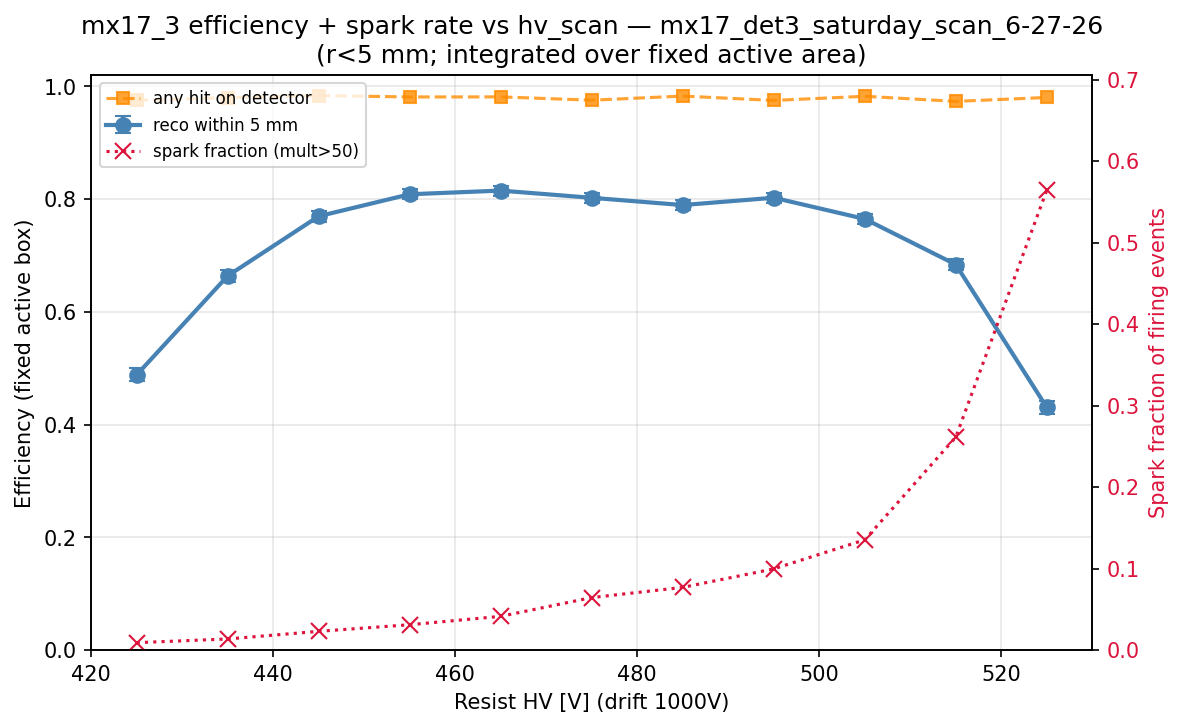
\includegraphics[width=0.495\textwidth]{efficiency_vs_hv_scan.png}
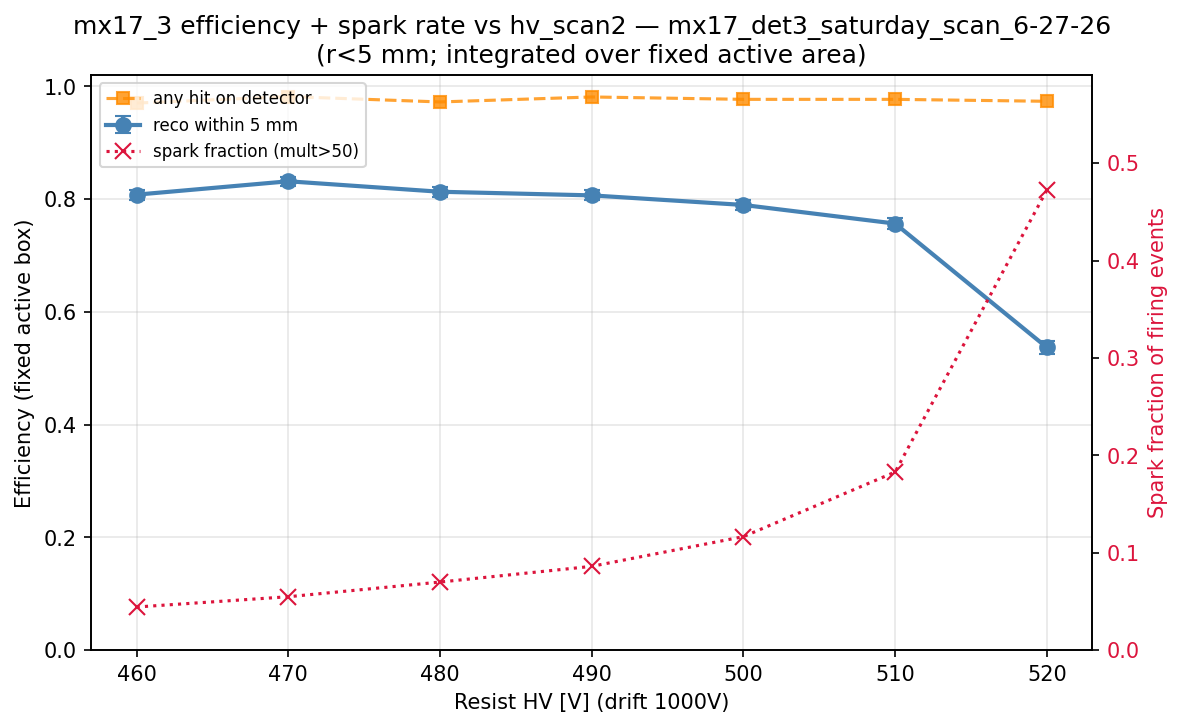
\includegraphics[width=0.495\textwidth]{efficiency_vs_hv_scan2.png}
\caption{Resist-HV scans (left: \SIrange{425}{525}{V}; right: fine repeat
\SIrange{460}{520}{V}).  Efficiency (blue), any-hit response (orange), spark
fraction (red crosses, right axis).}
\label{fig:hvscans}
\end{figure}

\begin{itemize}
  \item \textbf{Turn-on} at \SI{425}{V} (\SI{49}{\percent}) is complete by
        $\sim$\SI{455}{V};
  \item \textbf{plateau} \SIrange{455}{490}{V} at \SIrange{80}{83}{\percent}
        (best point \SI{83.2}{\percent} at \SI{470}{V} in the fine scan);
  \item \textbf{roll-off} above $\sim$\SI{505}{V} is driven entirely by
        sparking: the spark fraction climbs from \SI{4}{\percent} at
        \SI{470}{V} to \SI{56}{\percent} at \SI{525}{V} while the any-hit
        response stays $\approx\SI{98}{\percent}$ --- the detector is not
        going silent, its events are being destroyed by discharges;
  \item the \SI{490}{V} operating point of the long run sits on the plateau
        but already carries $\sim$\SI{9}{\percent} spark fraction;
        \SIrange{470}{480}{V} gives the same efficiency at half the spark
        rate and is the recommended setting.
\end{itemize}

%=====================================================================
\section{The analysis at a glance: what changed between the simple and
         the full-waveform treatment}
%=====================================================================
\label{sec:atglance}

This note went through three major revisions as the analysis deepened.
This section collects, in one place, every velocity estimator that was
tried, what information it uses, where its bias comes from, and what it
returned --- and then compares the physics conclusions of the simple
analysis with the final ones.

\subsection{Every estimator, one table}

\begin{table}[H]
\centering\footnotesize
\setlength{\tabcolsep}{4pt}%
\begin{tabular}{llllS[table-format=2.1]}
\toprule
estimator & uses & hidden assumption / bias & script &
{$\vd$(\SI{1000}{V})} \\
\midrule
$\sigma$-scan (production) & width of $|\thref|{-}|\thdet|$ &
  offset-free correlation; folds signs & prod. & 32.3 \\
ridge fit & slope of $S$ vs $\tan\thref$ &
  angle-\emph{independent} spreading & 13/14 & 28.1 \\
waveform re-timing & raw pulses, 4 time defs &
  ladder is linear (it is not) & 24 & 29.5 \\
endpoints / core OLS & cluster ends / core times &
  end times faithful (shared) & 22 & 29.8 \\
\textbf{geometry} & extent[mm] vs $\tan\thref$, $\div\,\Tsat$ &
  $w'$ small (toy-validated) & 21/23 & \bfseries 33.9 \\
toy-MC closure & simulation, all observables &
  model completeness & 25 & 34.0 \\
\textbf{unshared time fit} & waveforms after unsharing &
  sharing kernel from data & 26/27 & \bfseries 33.5 \\
\bottomrule
\end{tabular}
\caption{All drift-velocity estimators applied to the 2.4\,h run.  The two
bold entries are independent (one uses no time fit, the other no geometry)
and agree; every plain time-based fit clusters \SIrange{15}{20}{\percent}
low, for the single physical reason of Fig.~\ref{fig:sharingdiag}.}
\label{tab:estimators}
\end{table}

The decisive structural facts, in the order they were established:
\begin{enumerate}
  \item the ridge fit's flat-residual check is \emph{mathematically blind}
        to an angle-dependent spreading term (a linear $w(\tan\theta)$ is
        exactly degenerate with a change of $\vd$) --- so its agreement
        with itself proved nothing;
  \item the cluster-extent slope is the only observable with no time axis:
        \SI{23.2}{mm} per unit tan, cleanly between the ridge-implied
        \SI{19.4}{mm} and the mechanical \SI{30}{mm} --- the first
        model-independent sign that the time fits were biased;
  \item the raw waveforms showed the per-strip times are \emph{faithful}
        (four independent estimators agree) but the ladder is S-shaped ---
        the bias is signal physics, not algorithmic;
  \item vertical tracks measure the sharing directly
        ($c_1\approx0.5$!), the toy MC reproduces every observable with it
        and certifies the geometry estimator, and unsharing the waveforms
        makes the time fits agree with geometry --- closing the loop three
        independent ways.
\end{enumerate}

\subsection{Physics conclusions: before vs after}

\begin{table}[H]
\centering\small
\setlength{\tabcolsep}{5pt}%
\begin{tabular}{lll}
\toprule
quantity & simple analysis (rev.\ 1--2) & full waveform analysis (final) \\
\midrule
$\vd$(\SI{1000}{V}) & \SIrange{28}{32}{\umns} & $\SI{34\pm1.5}{\umns}$ \\
drift field scale & $E=V/\SI{1.94}{cm}$, then $V/\SI{3.0}{cm}$
  & $E=V/\SI{3.0}{cm}$ \\
``gap'' from $\vd\Tsat$ & \SI{19.4}{mm}, read as geometric
  & \SI{23}{mm} recorded column of a \SI{30}{mm} gap \\
gas & 2--2.5\,\% H$_2$O (``water-saturated''),
  & \SIrange{1.0}{1.1}{\percent} H$_2$O + $\sim$\SI{1}{\percent} air \\
  & briefly Ar/CO$_2$ 90/10 & (RMS \SI{0.84}{\umns}; CO$_2$ excluded) \\
attachment & $\lambda\approx\SIrange{13}{15}{mm}$, 0.2--0.4\,\% O$_2$
  & $\lambda\approx\SIrange{16}{18}{mm}$, 0.15--0.25\,\% O$_2$ \\
angle bias (plateau) & $\pm$\SIrange{4}{5}{\degree} (uncorrected)
  & \SI{0.19}{\degree} (unshared + calibrated) \\
angular resolution & \SIrange{1.5}{2}{\degree}, unusable
  $|\theta|\lesssim\SIrange{5}{7}{\degree}$
  & \SI{1.9}{\degree}, usable down to $\sim$\SIrange{3}{4}{\degree} \\
charge sharing & unknown (folded into ``$w$'')
  & measured: $c_1=0.45/0.52$, $c_2=0.05/0.15$, $+\SI{69}{ns}$ \\
\bottomrule
\end{tabular}
\caption{Side-by-side comparison of conclusions.  The off-diagonal
mechanism (Sec.~\ref{sec:offdiag}), the alignment, the position resolution
and the resist-scan results were correct from the start and did not
change.}
\label{tab:beforeafter}
\end{table}

Two lessons worth keeping.  First, a bias that afflicts \emph{every}
member of a family of estimators (here: all time-based fits) is invisible
to internal consistency checks within that family --- it took an
observable from outside the family (the mm-space extent) to expose it.
Second, the resistive-strip charge sharing at the 50\,\% level is a
first-order feature of this detector's raw data, not a small correction:
any timing-based quantity computed without accounting for it inherits a
double-digit-percent bias.

\subsection{Out-of-sample validation on det2}
\label{sec:det2val}

The entire chain was re-run from scratch on an independent detector:
\texttt{mx17\_2} (FEU 6/8, top slot) in the 6-22 overnight run --- same gas
line, same design, five days earlier, decoded waveforms pulled from the
lxplus archive (\texttt{29\_det2\_validation.py}).  Nothing from det3 was
reused except the method.

\begin{table}[H]
\centering\small
\begin{tabular}{lccl}
\toprule
observable & det3 (6-27) & det2 (6-22) & verdict \\
\midrule
sharing $c_1$ ($x$/$y$)      & 0.45 / 0.52 & 0.43 / 0.52 & \textbf{reproduced} \\
sharing $c_2$ ($x$/$y$)      & 0.05 / 0.15 & 0.06 / 0.20 & reproduced ($y$: RC direction) \\
neighbour delay              & $+\SI{69}{ns}$ & $+$74--85\,\si{ns} & reproduced \\
$\vd^{\mathrm{geom}}$ [\si{\umns}] & 33.9 & 35.0 / 30.8 ($x$/$y$) & consistent \\
$\vd$ unshared [\si{\umns}]  & 33.8 / 32.9 & \textbf{35.0 / 35.3} & \textbf{converges, matches} \\
$\lambda_{\mathrm{att}}$ [mm] & 16--18 & $\approx$40 & \emph{differs} (see text) \\
recorded column [mm]         & $\approx$23 & $\approx$25--26 & deeper, as $\lambda$ implies \\
\bottomrule
\end{tabular}
\caption{Out-of-sample test of the full chain on det2.}
\label{tab:det2val}
\end{table}

The sharing constants and the unshared velocity transfer perfectly ---
$c_{1,2}$ are properties of the common strip design, and the drift velocity
of the shared gas line is confirmed at $\vd(\SI{1000}{V}) \approx
\SIrange{34}{35}{\umns}$ on a second detector by two estimators.  The
\emph{attachment}, however, does not transfer: det2's amplitude decay is
$\sim$2.5$\times$ weaker ($\lambda\approx\SI{40}{mm}$) and its recorded
column correspondingly deeper.  This sharpens the contamination model
rather than weakening it: the drift \emph{velocity} is set by the water
(identical in both detectors --- consistent with a common line and similar
outgassing equilibrium), while the \emph{attachment} is set by O$_2$,
which evidently differs between detector volumes or evolved over the five
days between the runs.  Water without oxygen slows the gas but does not
capture electrons --- exactly what det2 shows.  A per-detector O$_2$
budget (from each detector's own amplitude-vs-depth curve) is therefore
part of any future gas accounting.

\subsection{The fleet-and-time survey: det3 dried out during the week}
\label{sec:fleetsurvey}

Extending the two gas observables to \emph{every} June run with a cached
analysis (\texttt{30\_fleet\_gas\_survey.py}) --- with each run's actual
drift HV decoded from its \texttt{hv\_monitor.csv} (channel mapping
calibrated on the Saturday run) --- turns the survey into a time series
(Fig.~\ref{fig:fleetsurvey}).  Converting each measured $\vd$ at its true
field into an implied water fraction via the Magboltz grid:

\begin{table}[H]
\centering\small
\begin{tabular}{llS[table-format=4.0]S[table-format=2.1]lS[table-format=2.0]l}
\toprule
date & det (slot) & {drift [V]} & {$\vd$ [\si{\umns}]} & H$_2$O
     & {$\lambda$ [mm]} & note \\
\midrule
6-22  & det3 (test)   &  986 &  8.7 & $>$3\,\% & 37 & \textbf{water-saturated} \\
6-22  & det3 (bottom) & 1000 &  9.2 & $>$3\,\% & 16 & \textbf{water-saturated} \\
6-22  & det2 (top)    & 1000 & 32.9 & 1.05\,\% & 42 & dry, low O$_2$ \\
6-23  & det3 (bottom) &  600 &  1.1 & {---} & {---} & broken point (excluded) \\
6-23  & det4 (top)    &  600 & 23.6 & 0.76\,\% & 29 & \\
6-24  & det4          &  600 & 21.8 & 0.83\,\% & 25 & \\
6-25  & det3          &  500$^*$ & 18.8 & 0.75--1.2\,\% & 9 & dried; $^*$HV ambiguous \\
6-26  & det6 (bottom) &  700 & 19.1 & 1.19\,\% & 9 & low trust ($x/y$ split 40\,\%) \\
6-26  & det7 (top)    &  700 & 29.2 & 0.73\,\% & 9 & low trust \\
6-27  & det3 (top)    & 1000 & 32.8 & 1.05\,\% & 23 & this note's reference \\
6-27n & det3 (top)    &  999 & 34.3 & 0.97\,\% & 22 & p2 run, 45k events \\
\bottomrule
\end{tabular}
\caption{Fleet-and-time survey.  $\lambda$ values are at each run's own
field (attachment lengthens with $E$), so cross-run O$_2$ comparisons use
the Magboltz field dependence.}
\label{tab:fleetsurvey}
\end{table}

\begin{figure}[H]
\centering
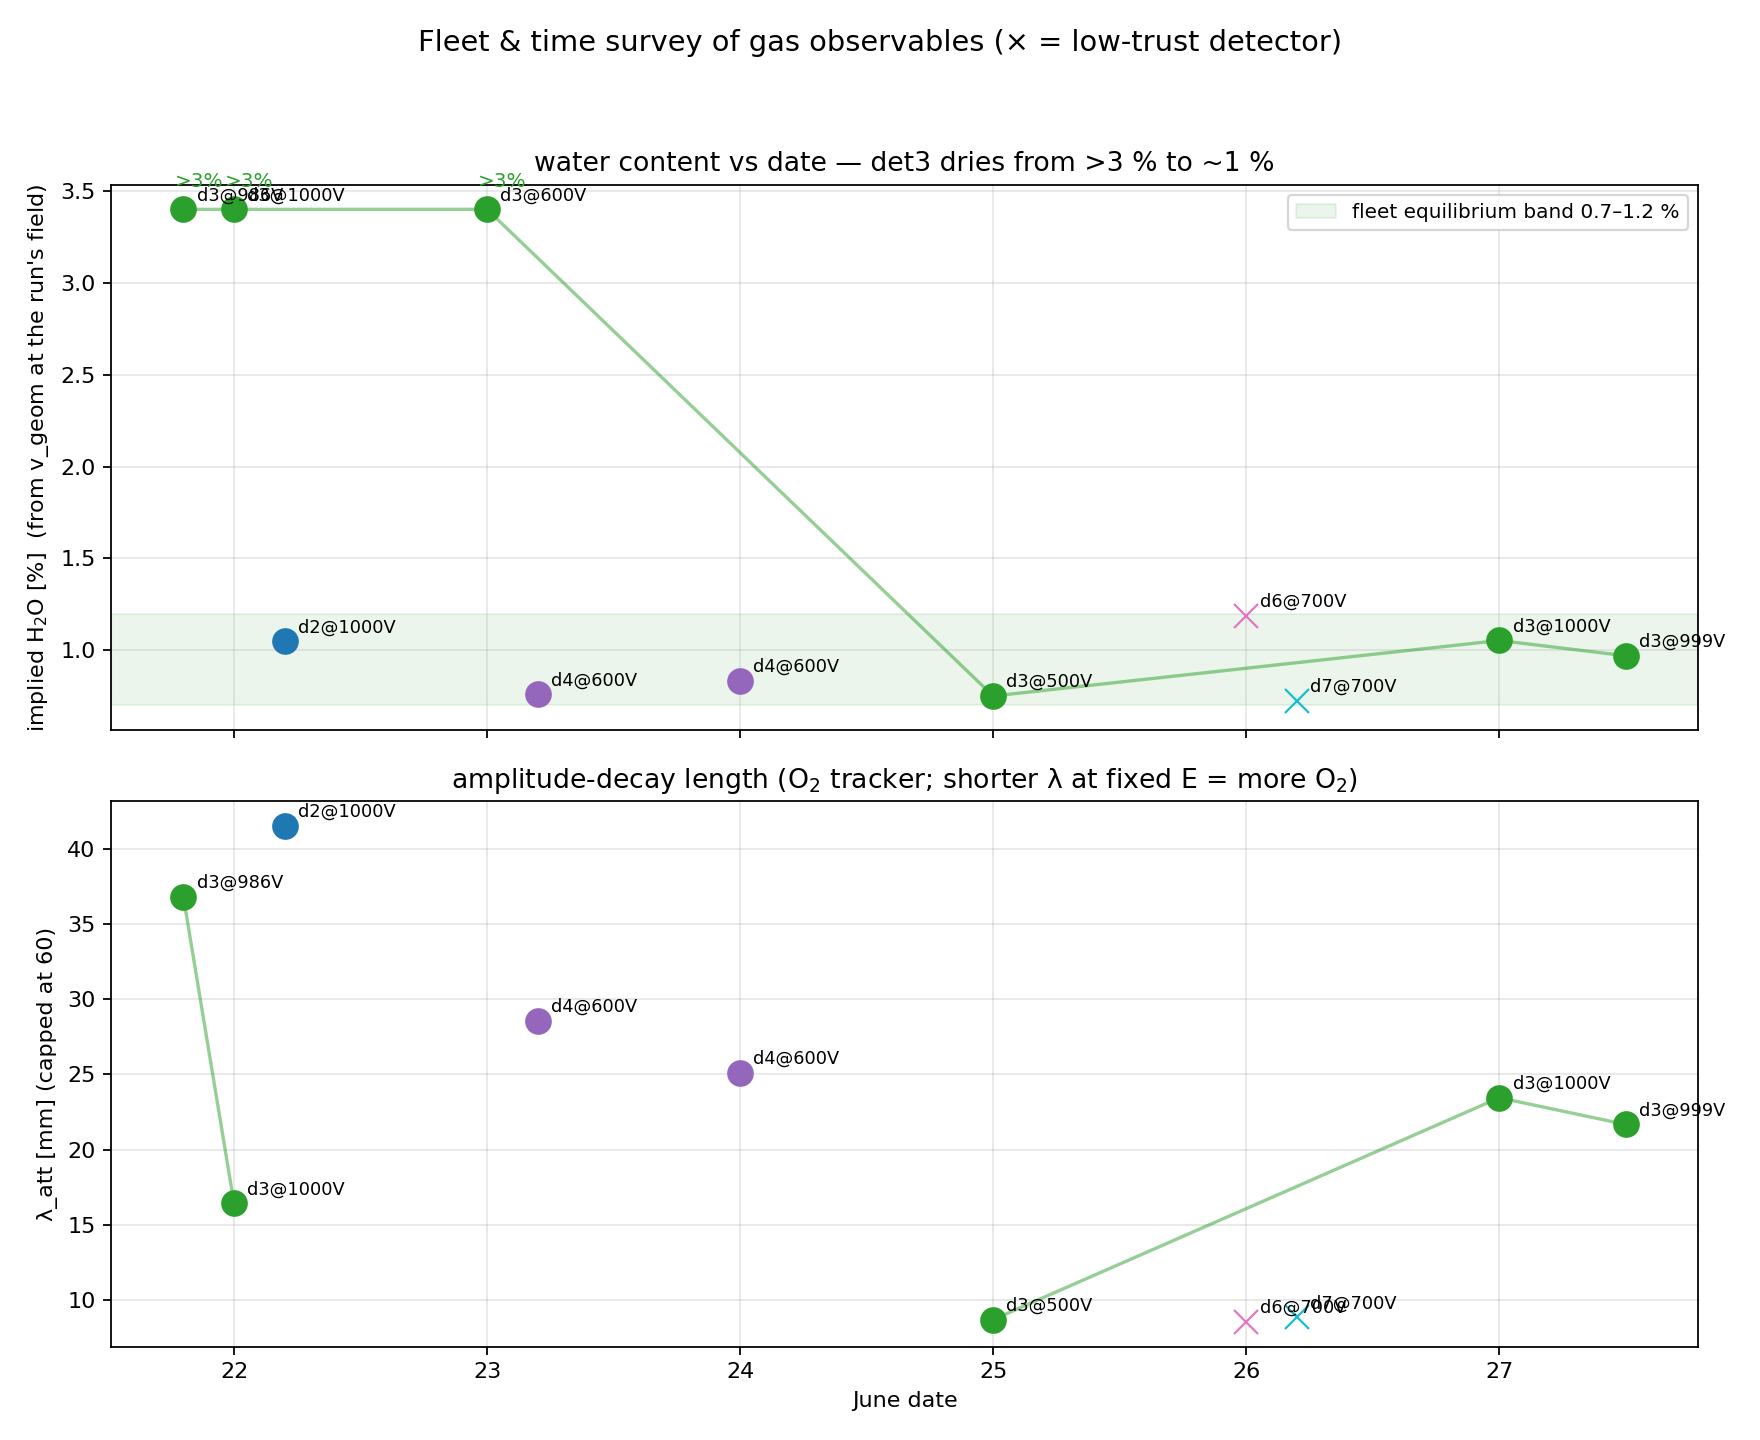
\includegraphics[width=0.9\textwidth]{fleet_gas_survey.png}
\caption{Implied water fraction (top) and amplitude-decay length (bottom)
per detector per date.  det3 (line) dries from beyond the 3\,\% grid edge
on 6-22 to the fleet band by 6-25 and is stable at $\approx$1\,\% on 6-27;
every other detector-day sits in the 0.7--1.2\,\% band.}
\label{fig:fleetsurvey}
\end{figure}

Findings:
\begin{itemize}
  \item \textbf{det3 was water-saturated early in the week} ($\vd \approx
        \SI{9}{\umns}$ at \SI{333}{V/cm} on 6-22, in \emph{two} independent
        runs --- below even the 3\,\% Magboltz curve) and \textbf{dried to
        the fleet equilibrium of $\approx$1\,\%} by 6-25, stable through
        both 6-27 runs (1.05/0.97\,\%).  The flushing worked; it just took
        days.  Amusingly, the first revision of this note concluded
        ``2--2.5\,\% water-saturated gas'' from biased-velocity reasoning
        --- which happens to be a fair description of det3 \emph{earlier
        that week}.
  \item \textbf{The fleet equilibrium is $\approx$1\,\% H$_2$O}
        ($0.7$--$1.2$\,\% across det2/3/4/6/7 and dates) --- a property of
        the gas system, with per-volume scatter.
  \item \textbf{O$_2$ is per-detector and highest in the newest installs}:
        det6/7 (installed last, 6-26) show $\lambda\approx\SI{9}{mm}$ at
        \SI{233}{V/cm} ($\approx$2\,\% air-equivalent), det3 sits at
        $\approx$1\,\% air, det2/det4 at $\approx$0.5\,\%.  Air flushes
        out over time just as the water does.
  \item The same-day det3 pairs (6-22 test/overnight; 6-27
        Saturday/p2-night) agree internally --- the strongest evidence that
        the run-to-run differences are real gas evolution, not method
        noise.  det6's 40\,\% $x$/$y$ velocity split justifies the low
        trust assigned to it; det7 is marginal (12\,\%).
\end{itemize}

%=====================================================================
\section{Summary and follow-ups}
%=====================================================================

\subsection{Summary}

\begin{enumerate}
  \item \textbf{Off-diagonal angle correlation --- solved.}  It is the
        additive charge-spreading bias
        $\tan\thdet = \tan\thref \pm w/z_{\mathrm{rec}}$
        ($w\approx\SI{2}{mm}$): a detector-family constant.  Not a
        rotation; not a bug.  It also explains the
        $|\thdet|\gtrsim\SI{5}{\degree}$ exclusion gap and the horizontal
        arms at $\thref\approx0$.
  \item \textbf{Drift velocity --- measured, after an estimator odyssey.}
        Every time-based fit (production and waveform-level alike) is
        biased low \SIrange{10}{20}{\percent} by prompt charge sharing
        between resistive strips --- demonstrated in the raw waveforms and
        closed with a signal-formation toy MC.  The validated
        \emph{geometry} estimator (extent slope / time-span plateau) gives
        $\vd(\SI{1000}{V}) = \SI{34\pm1.5}{\umns}$, full curve in
        Table~\ref{tab:vdrift}, \SIrange{1}{3}{\percent} statistical per
        15-minute point.
  \item \textbf{Drift gap --- \SI{30}{mm} mechanical, $\approx\SI{23}{mm}$
        recorded.}  The recorded column (geometry: \SIrange{21.5}{23.5}{mm},
        constant with field) is where drifting charge falls below threshold,
        not the electrode spacing; the strip amplitude decays with drift
        \emph{depth} ($\lambda\approx\SIrange{16}{18}{mm}$, one universal
        curve for all fields) --- charge from the top of the gap is lost to
        attachment in the contaminated gas.
  \item \textbf{Gas --- air/moisture contamination, quantified.}  The
        geometry $\vd(E)$ at $E=V/\SI{3.0}{cm}$ matches Ar/iso 95/5 +
        \SIrange{1.0}{1.1}{\percent} H$_2$O (+$\sim$\SI{1}{\percent} air) at
        RMS \SI{0.84}{\umns}; the attachment length independently returns
        the same $\sim$\SI{1}{\percent} air.  Clean gas, mixing errors and
        the Ar/CO$_2$ wrong bottle are excluded.
  \item \textbf{Tracking --- fixed on the existing data.}  Waveform
        unsharing (sharing constants measured from vertical tracks) plus
        one additive calibration constant per plane brings the micro-TPC
        angles to \SI{0.19}{\degree} plateau bias and \SI{1.9}{\degree}
        resolution, usable down to $\sim$\SIrange{3}{4}{\degree}
        (Secs.~\ref{sec:timing}, Fig.~\ref{fig:anglecal}).
  \item \textbf{Operating point.}  det3: resist \SIrange{470}{480}{V}
        (same efficiency as \SI{490}{V}, half the sparks), drift
        $\geq\SI{700}{V}$ (readout-window constraint), \SI{80}{\percent}
        reconstruction efficiency, \SI{0.83}{}/\SI{0.92}{mm} core
        resolution (position resolution is unaffected by the timing bias).
\end{enumerate}

\subsection{Follow-ups}

The campaign data are final --- no re-runs and no fresh-gas measurements
are possible --- so every follow-up below works on the existing files.
\begin{enumerate}
  \item \textbf{Production integration of unsharing (done offline; to be
        promoted).}  The correction chain is validated end-to-end in
        \texttt{26}--\texttt{28\_*.py}; promoting it into the
        decoded$\to$hits converter (\texttt{mm\_processor}) amounts to one
        linear pre-filter per event and FEU --- a banded solve of
        $(\mathbb{1}+\alpha c_1E_{\pm1}+\alpha c_2E_{\pm2})$ with the
        delayed remainder handled causally --- with $(c_1, c_2, \alpha)$
        as per-detector calibration constants measured from any run's
        vertical tracks.  Downstream code is unchanged; the min-strips cut
        must drop $4\to3$ (unshared clusters are narrower).  Then wire the
        geometry $\vd$ and the additive angle calibration into
        \texttt{03\_alignment\_and\_tpc.py}.
  \item \textbf{Cluster template fit (next algorithmic step, if plateau
        resolution matters).}  The maximum-information estimator: fit each
        cluster's full strip$\times$sample matrix with a model =
        track-slope parameter + per-strip charges, with the sharing kernel
        and shaper \emph{fixed} to their measured forms.  The toy MC
        (\texttt{25\_*.py}) already contains every ingredient to prototype
        and closure-test it.  Given that the current \SI{1.9}{\degree}
        plateau is dominated by diffusion in the contaminated gas and the
        \SI{60}{ns} sampling, gains are expected to be moderate ---
        worthwhile mainly for the small-angle region.
  \item \textbf{Out-of-sample validation on other detectors}: run the
        geometry estimator and (where decoded data exist on lxplus) the
        unsharing chain on the det2/6/7 June runs --- same gas line, so the
        same $\vd(E)$, $\lambda_{\mathrm{att}}$ and sharing constants are
        predicted.
  \item Mechanics/paperwork: confirm the \SI{30}{mm} drift-gap drawing;
        confirm the DREAM sampling period (\SI{60}{ns}), which sets the
        absolute time scale of everything here.
  \item The Saturday long run is \emph{complete} at \SI{141}{min}; for more
        det3 statistics use the p2 overnight run (53k rays), to which the
        unsharing chain applies once its decoded files are pulled.
\end{enumerate}

\vspace{4mm}
{\sloppy
\noindent\textbf{Reproducibility.}  Run key \texttt{sat\_det3} in
\texttt{mx\_june\_cosmic\_qa/qa\_config.py}.  Scripts:
\texttt{13\_tpc\_angle\_bias.py} (bias study),
\texttt{14\_drift\_velocity\_scan.py} (ridge fit),
\texttt{15\_drift\_velocity\_vs\_magboltz.py} (gas comparison),
\texttt{16}--\texttt{19} (gap and attachment tests),
\texttt{20\_ridge\_systematics.py}--\texttt{23\_core\_geometry\_vdrift.py}
(geometry estimator), \texttt{24\_waveform\_investigation.py} and
\texttt{25\_signal\_formation\_toy.py} (waveforms and closure),
\texttt{26\_unsharing\_analysis.py}--\texttt{28\_angle\_calibration.py}
(unsharing prototype, kernel refinement, angle calibration), and
\texttt{mm\_drift\_velocity\_\{table,candidates\}.py},
\texttt{mm\_attachment\_\{table,air\_candidates\}.py},
\texttt{mm\_townsend\_compare.py},
\texttt{mm\_water\_grid\_lxplus.py} in
\texttt{garfield\_sim/} (Magboltz, local + lxplus).  Outputs live under
\texttt{Analysis/mx17\_det3\_saturday\_scan\_6-27-26/} in the cosmic-bench
data tree.\par}

\end{document}
